%%%%%%%%%%%%%%%%%%%%%%%%%%%%%%%%%%%%%%%%%%%%%%%%%%%%%%%%%%%%%%%%%%%%%%%
%
%  A small sample UNSW Honours Thesis file.
%  Any questions to Ian Doust i.doust@unsw.edu.au
%
% Edited CSG 11.9.2015, use some of Gery's ideas for front matter; add a conclusion chapter.
%%%%%%%%%%%%%%%%%%%%%%%%%%%%%%%%%%%%%%%%%%%%%%%%%%%%%%%%%%%%%%%%%%%%%%%
% 
%  The first part pulls in a UNSW Thesis class file.  This one is
%  slightly nonstandard and has been set up to do a couple of
%  things automatically
%

\documentclass[honours,12pt,twoside]{unswthesis}

\usepackage{afterpage}
\usepackage{amsfonts}
\usepackage{amsmath}
\usepackage{amssymb}
\usepackage{amsthm}
\usepackage[english]{babel}
\usepackage{graphicx}
\usepackage{natbib}
\usepackage[utf8]{inputenc}
\usepackage{latexsym}
\usepackage{url}
\usepackage{todonotes}
\usepackage{tikz}
\usepackage{pdfpages}
\usetikzlibrary{arrows}
\usepackage{float}

\usepackage{booktabs}
\renewcommand{\arraystretch}{1.2}


%%%%%%%%%%%%%%%%%%%%%%%%%%%%%%%%%%%%%%%%%%%%%%%%%%%%%%%%%%%%%%%%%
%
%  The following are some simple LaTeX macros to give some
%  commonly used letters in funny fonts. You may need more or less of
%  these
%
\newcommand{\R}{\mathbb{R}}
\newcommand{\Q}{\mathbb{Q}}
\newcommand{\C}{\mathbb{C}}
\newcommand{\N}{\mathbb{N}}
\newcommand{\F}{\mathbb{F}}
\newcommand{\PP}{\mathbb{P}}
\newcommand{\T}{\mathbb{T}}
\newcommand{\Z}{\mathbb{Z}}
\newcommand{\B}{\mathfrak{B}}
\newcommand{\BB}{\mathcal{B}}
\newcommand{\M}{\mathfrak{M}}
\newcommand{\X}{\mathfrak{X}}
\newcommand{\Y}{\mathfrak{Y}}
\newcommand{\CC}{\mathcal{C}}
\newcommand{\E}{\mathbb{E}}
\newcommand{\cP}{\mathcal{P}}
\newcommand{\cS}{\mathcal{S}}
\newcommand{\A}{\mathcal{A}}
\newcommand{\ZZ}{\mathcal{Z}}

%%%%%%%%%%%%%%%%%%%%%%%%%%%%%%%%%%%%%%%%%%%%%%%%%%%%%%%%%%%%%%%%%%%%%
%
% The following are much more esoteric commands that I have left in
% so that this file still processes. Use or delete as you see fit
%
\newcommand{\bv}[1]{\mbox{BV($#1$)}}
\newcommand{\comb}[2]{\left(\!\!\!\begin{array}{c}#1\\#2\end{array}\!\!\!\right)
}
\newcommand{\Lat}{{\rm Lat}}
\newcommand{\var}{\mathop{\rm var}}
\newcommand{\Pt}{{\mathcal P}}
\def\tr(#1){{\rm trace}(#1)}
\def\Exp(#1){{\mathbb E}(#1)}
\def\Exps(#1){{\mathbb E}\sparen(#1)}
\newcommand{\floor}[1]{\left\lfloor #1 \right\rfloor}
\newcommand{\ceil}[1]{\left\lceil #1 \right\rceil}
\newcommand{\hatt}[1]{\widehat #1}
\newcommand{\modeq}[3]{#1 \equiv #2 \,(\text{mod}\, #3)}
\newcommand{\rmod}{\,\mathrm{mod}\,}
\newcommand{\p}{\hphantom{+}}
\newcommand{\vect}[1]{\mbox{\boldmath $ #1 $}}
\newcommand{\reff}[2]{\ref{#1}.\ref{#2}}
\newcommand{\psum}[2]{\sum_{#1}^{#2}\!\!\!'\,\,}
\newcommand{\bin}[2]{\left( \begin{array}{@{}c@{}}
				#1 \\ #2
			\end{array}\right)	}
%
%  Macros - some of these are in plain TeX (gasp!)
%
\newcommand{\be}{($\beta$)}
\newcommand{\eqp}{\mathrel{{=}_p}}
\newcommand{\ltp}{\mathrel{{\prec}_p}}
\newcommand{\lep}{\mathrel{{\preceq}_p}}
\def\brack#1{\left \{ #1 \right \}}
\def\bul{$\bullet$\ }
\def\cl{{\rm cl}}
\let\del=\partial
\def\enditem{\par\smallskip\noindent}
\def\implies{\Rightarrow}
\def\inpr#1,#2{\t \hbox{\langle #1 , #2 \rangle} \t}
\def\ip<#1,#2>{\langle #1,#2 \rangle}
\def\lp{\ell^p}
\def\maxb#1{\max \brack{#1}}
\def\minb#1{\min \brack{#1}}
\def\mod#1{\left \vert #1 \right \vert}
\def\norm#1{\left \Vert #1 \right \Vert}
\def\paren(#1){\left( #1 \right)}
\def\qed{\hfill \hbox{$\Box$} \smallskip}
\def\sbrack#1{\Bigl \{ #1 \Bigr \} }
\def\ssbrack#1{ \{ #1 \} }
\def\smod#1{\Bigl \vert #1 \Bigr \vert}
\def\smmod#1{\bigl \vert #1 \bigr \vert}
\def\ssmod#1{\vert #1 \vert}
\def\sspmod#1{\vert\, #1 \, \vert}
\def\snorm#1{\Bigl \Vert #1 \Bigr \Vert}
\def\ssnorm#1{\Vert #1 \Vert}
\def\sparen(#1){\Bigl ( #1 \Bigr )}

\newcommand\blankpage{%
    \null
    \thispagestyle{empty}%
    \addtocounter{page}{-1}%
    \newpage}
    
%%%%%%%%%%%%%%%%%%%%%%%%%%%%%%%%%%%%%%%%%%%%%%%%%%%%%%%%%%%%%%
%
% These environments allow you to get nice numbered headings
%  for your Theorems, Definitions etc.  
%
%  Environments
%
%%%%%%%%%%%%%%%%%%%%%%%%%%%%%%%

\newtheorem{theorem}{Theorem}[section]
\newtheorem{lemma}[theorem]{Lemma}
\newtheorem{proposition}[theorem]{Proposition}
\newtheorem{corollary}[theorem]{Corollary}
\newtheorem{conjecture}[theorem]{Conjecture}
\newtheorem{definition}[theorem]{Definition}
\newtheorem{example}{Example}
\newtheorem{remark}[theorem]{Remark}
\newtheorem{question}[theorem]{Question}
\newtheorem{notation}[theorem]{Notation}
\numberwithin{equation}{section}


%%%%%%%%%%%%%%%%%%%%%%%%%%%%%%%%%%%%%%%%%%%%%%%%%%%%%%%%%%%%%%%%%%
%
%  If you've got some funny special words that LaTeX might not
% hyphenate properly, you can give it a helping hand:
%
%\hyphenation{Mar-cin-kie-wicz Rade-macher}

%%%%%%%%%%%%%%%%%%%%%%%%%%%%%%%%%%%%%%%%%%%%%%%%%%%%%%%%%%%%%%%%%%
% 
% OK...Now we get to some actual input.  The first part sets up
% the title etc that will appear on the front page
%
%%%%%%%%%%%%%%%%%%%%%%%%%%%%%%%%%%%%%%%%%%%%%%%%%%%%%%%%%%%%%%%%%

\title{The Automated Detection of Lacunes and Perivascular Spaces in MRI}

\authornameonly{Melinda Mortimer}

\author{\Authornameonly\\{\bigskip}Supervisors: Dr Pierre Lafaye de Micheaux \& Associate Professor Wei Wen}


\copyrightfalse
\figurespagefalse
\tablespagefalse

%%%%%%%%%%%%%%%%%%%%%%%%%%%%%%%%%%%%%%%%%%%%%%%%%%%%%%%%%%%%%%%%%
%
%  And now the document begins
%  The \beforepreface and \afterpreface commands puts the
%  contents page etc in
%
%%%%%%%%%%%%%%%%%%%%%%%%%%%%%%%%%%%%%%%%%%%%%%%%%%%%%%%%%%%%%%%%%%

\begin{document}

\beforepreface

\afterpage{\blankpage}

% plagiarism

\prefacesection{Plagiarism statement}

\vskip 10pc \noindent I declare that this thesis is my
own work, except where acknowledged, and has not been submitted for
academic credit elsewhere. 

\vskip 2pc  \noindent I acknowledge that the assessor of this
thesis may, for the purpose of assessing it:
\begin{itemize}
\item Reproduce it and provide a copy to another member of the University; and/or,
\item Communicate a copy of it to a plagiarism checking service (which may then retain a copy of it on its database for the purpose of future plagiarism checking).
\end{itemize}

\vskip 2pc \noindent I certify that I have read and understood the University Rules in
respect of Student Academic Misconduct, and am aware of any potential plagiarism penalties which may 
apply.\vspace{24pt}

\vskip 2pc \noindent By signing this declaration I am agreeing to the statements and conditions above.
\vskip 2pc
Signed: \rule{7cm}{0.25pt} \hfill Date: \rule{4cm}{0.25pt}

\afterpage{\blankpage}

% Acknowledgements are optional


\prefacesection{Acknowledgements}

%{\bigskip}By far the greatest thanks must go to my supervisor for
%the guidance, care and support they provided. 
%
%{\bigskip\noindent}Thanks must also go to Emily, Michelle, John and Alex who helped by
%proof-reading the document in the final stages of preparation.
%
%{\bigskip\noindent}Although I have not lived with them for a number of years, my family also deserve many thanks for their encouragement.
%
%{\bigskip\noindent} Thanks go to Robert Taggart for allowing his thesis style to be shamelessly copied.
%
%{\bigskip\bigskip\bigskip\noindent} Fred Flintstone, 2 November 2015.

\afterpage{\blankpage}

% Abstract

\prefacesection{Abstract}

%This thesis is a coherent presentation of a quest to generalise three classical
%theorems that were discovered in the 1920s, 1930s and 1940s. Their analogues are
%the product of a conglomeration of ideas that straddle the 1980s and 1990s and
%the application of these new results brings the story into the twenty-first
%century.
\afterpage{\blankpage}

%%%%%%%%%%%%%%%%%%%%%%%%%%%%%%%%%%%%%%%%%%%%%%%%%%%%%%%%%%%%%%%%%%
%
% Now we can start on the first chapter
% Within chapters we have sections, subsections and so forth
%
%%%%%%%%%%%%%%%%%%%%%%%%%%%%%%%%%%%%%%%%%%%%%%%%%%%%%%%%%%%%%%%%%%
%%%%%%%%%%%%%%%%%     CONTENT STARTS HERE!!!     %%%%%%%%%%%%%%%%%
%%%%%%%%%%%%%%%%%%%%%%%%%%%%%%%%%%%%%%%%%%%%%%%%%%%%%%%%%%%%%%%%%%

\afterpage{\blankpage}

%\documentclass[honours,12pt,twoside]{unswthesis}

\usepackage{afterpage}
\usepackage{amsfonts}
\usepackage{amsmath}
\usepackage{amssymb}
\usepackage{amsthm}
\usepackage[english]{babel}
\usepackage{graphicx}
\usepackage{natbib}
\usepackage[utf8]{inputenc}
\usepackage{latexsym}
\usepackage{url}
\usepackage{todonotes}
\usepackage{tikz}
\usepackage{pdfpages}
\usetikzlibrary{arrows}
\usepackage{float}

\usepackage{booktabs}
\renewcommand{\arraystretch}{1.2}


%%%%%%%%%%%%%%%%%%%%%%%%%%%%%%%%%%%%%%%%%%%%%%%%%%%%%%%%%%%%%%%%%
%
%  The following are some simple LaTeX macros to give some
%  commonly used letters in funny fonts. You may need more or less of
%  these
%
\newcommand{\R}{\mathbb{R}}
\newcommand{\Q}{\mathbb{Q}}
\newcommand{\C}{\mathbb{C}}
\newcommand{\N}{\mathbb{N}}
\newcommand{\F}{\mathbb{F}}
\newcommand{\PP}{\mathbb{P}}
\newcommand{\T}{\mathbb{T}}
\newcommand{\Z}{\mathbb{Z}}
\newcommand{\B}{\mathfrak{B}}
\newcommand{\BB}{\mathcal{B}}
\newcommand{\M}{\mathfrak{M}}
\newcommand{\X}{\mathfrak{X}}
\newcommand{\Y}{\mathfrak{Y}}
\newcommand{\CC}{\mathcal{C}}
\newcommand{\E}{\mathbb{E}}
\newcommand{\cP}{\mathcal{P}}
\newcommand{\cS}{\mathcal{S}}
\newcommand{\A}{\mathcal{A}}
\newcommand{\ZZ}{\mathcal{Z}}

%%%%%%%%%%%%%%%%%%%%%%%%%%%%%%%%%%%%%%%%%%%%%%%%%%%%%%%%%%%%%%%%%%%%%
%
% The following are much more esoteric commands that I have left in
% so that this file still processes. Use or delete as you see fit
%
\newcommand{\bv}[1]{\mbox{BV($#1$)}}
\newcommand{\comb}[2]{\left(\!\!\!\begin{array}{c}#1\\#2\end{array}\!\!\!\right)
}
\newcommand{\Lat}{{\rm Lat}}
\newcommand{\var}{\mathop{\rm var}}
\newcommand{\Pt}{{\mathcal P}}
\def\tr(#1){{\rm trace}(#1)}
\def\Exp(#1){{\mathbb E}(#1)}
\def\Exps(#1){{\mathbb E}\sparen(#1)}
\newcommand{\floor}[1]{\left\lfloor #1 \right\rfloor}
\newcommand{\ceil}[1]{\left\lceil #1 \right\rceil}
\newcommand{\hatt}[1]{\widehat #1}
\newcommand{\modeq}[3]{#1 \equiv #2 \,(\text{mod}\, #3)}
\newcommand{\rmod}{\,\mathrm{mod}\,}
\newcommand{\p}{\hphantom{+}}
\newcommand{\vect}[1]{\mbox{\boldmath $ #1 $}}
\newcommand{\reff}[2]{\ref{#1}.\ref{#2}}
\newcommand{\psum}[2]{\sum_{#1}^{#2}\!\!\!'\,\,}
\newcommand{\bin}[2]{\left( \begin{array}{@{}c@{}}
				#1 \\ #2
			\end{array}\right)	}
%
%  Macros - some of these are in plain TeX (gasp!)
%
\newcommand{\be}{($\beta$)}
\newcommand{\eqp}{\mathrel{{=}_p}}
\newcommand{\ltp}{\mathrel{{\prec}_p}}
\newcommand{\lep}{\mathrel{{\preceq}_p}}
\def\brack#1{\left \{ #1 \right \}}
\def\bul{$\bullet$\ }
\def\cl{{\rm cl}}
\let\del=\partial
\def\enditem{\par\smallskip\noindent}
\def\implies{\Rightarrow}
\def\inpr#1,#2{\t \hbox{\langle #1 , #2 \rangle} \t}
\def\ip<#1,#2>{\langle #1,#2 \rangle}
\def\lp{\ell^p}
\def\maxb#1{\max \brack{#1}}
\def\minb#1{\min \brack{#1}}
\def\mod#1{\left \vert #1 \right \vert}
\def\norm#1{\left \Vert #1 \right \Vert}
\def\paren(#1){\left( #1 \right)}
\def\qed{\hfill \hbox{$\Box$} \smallskip}
\def\sbrack#1{\Bigl \{ #1 \Bigr \} }
\def\ssbrack#1{ \{ #1 \} }
\def\smod#1{\Bigl \vert #1 \Bigr \vert}
\def\smmod#1{\bigl \vert #1 \bigr \vert}
\def\ssmod#1{\vert #1 \vert}
\def\sspmod#1{\vert\, #1 \, \vert}
\def\snorm#1{\Bigl \Vert #1 \Bigr \Vert}
\def\ssnorm#1{\Vert #1 \Vert}
\def\sparen(#1){\Bigl ( #1 \Bigr )}

\newcommand\blankpage{%
    \null
    \thispagestyle{empty}%
    \addtocounter{page}{-1}%
    \newpage}
    
%%%%%%%%%%%%%%%%%%%%%%%%%%%%%%%%%%%%%%%%%%%%%%%%%%%%%%%%%%%%%%
%
% These environments allow you to get nice numbered headings
%  for your Theorems, Definitions etc.  
%
%  Environments
%
%%%%%%%%%%%%%%%%%%%%%%%%%%%%%%%

\newtheorem{theorem}{Theorem}[section]
\newtheorem{lemma}[theorem]{Lemma}
\newtheorem{proposition}[theorem]{Proposition}
\newtheorem{corollary}[theorem]{Corollary}
\newtheorem{conjecture}[theorem]{Conjecture}
\newtheorem{definition}[theorem]{Definition}
\newtheorem{example}{Example}
\newtheorem{remark}[theorem]{Remark}
\newtheorem{question}[theorem]{Question}
\newtheorem{notation}[theorem]{Notation}
\numberwithin{equation}{section}

%\begin{document}

\chapter{Introduction}\label{s-intro}

\section{Overview}\label{overview}

{\noindent} Cerebral Small Vessel Disease (SVD) describes a set of abnormalities affecting small blood vessels in the deep grey and white matter of the brain. The changes are particularly prevalent amongst the elderly, with SVD biomarkers appearing in over 90\% of MRI for those aged 60-90 years \cite{deLeeuwF-E2001Pocw}. SVD is the primary cause of over one fifth of ischaemic (oxygen-starved) strokes \cite{SmithStephen2002ARaA} and is a major cause of dementia and cognitive decline \cite{NorrvingBo2008Linb}.

Imaging markers of SVD include lacunes, enlarged perivascular spaces, white matter hyperintensities, microbleeds, recent small subcortical infarcts and brain atrophy \cite{WardlawJ.M.2013Nsfr}.

Current research is investigating the role of particular biomarkers in the advancement of SVD. Currently, it is not clear the extent to which SVD affects cognition, or which events are to blame. Consequently, there is the need for clear identification of biomarkers to ensure accurate analysis can be made.

The identification of SVD biomarkers in MRI (rating) is generally conducted by eye. The 3D image constructed by an MRI scan is made up of numerous 2D slices. Trained clinicians, with reference to STRIVE criterion \cite{WardlawJ.M.2013Nsfr}, examine each image slice for lesions and other features of interest. The coordinates, sizes and counts of these features are logged manually.

However, some neuroscientists have commented on the difficulty and reliability of these rating methods. Wardlaw et al. \cite{WardlawJm2013Mosc} advised caution when conducted inference as many of the features are difficult to identify. This was especially the case for research coordinated prior to 2013, before the STRIVE criterion was established \cite{WardlawJ.M.2013Nsfr}.

Several attempts have been made to improve the reliability of visual rating, with moderate success \cite{AdamsH.H.Hieab2013RMfD, PotterGillian2015CPSV}. However intra-rater and inter-rater percentage agreements are still low for brain regions with a higher frequency of lacunes and perivascular spaces, such as the basal ganglia. In the trial by Potter et al. \cite{PotterGillian2015CPSV},  the intra-rater and inter-rater agreements for the basal ganglia were 0.54-0.68 and 0.65-0.77 respectively. This was considered an improvement, however the extent of the remaining inconsistencies means that caution must be taken when drawing conclusions.

Lacunes are of particular interest as the role of lacunes and perivascular spaces is still under consideration. In one instance, Benjamin et al. \cite{BenjaminJ.Philip2018LIbN} argue that it is only lacunes, rather than perivascular spaces, that influence cognitive decline. They suspect that previous observed influence of perivascular spaces may have been the result of incorrect classification during the rating process.

To allow for more accurate, efficient and consistent image rating of lacunes and perivascular spaces, this paper attempts to automate the process via machine learning. As developments with machine learning are fairly recent, there have been a limited number of previous attempts.

The first attempts at automated lacune detection were conducted by Yokoyama et al. \cite{YokoyamaRyujiro2002Aado}, primarily focussing on the definition of lacunes in identification. Their study showed promising results, but with a high proportion of false-positives - 1.77 per image.

By 2007, their model had undergone a number of revisions. Uchiyama et al. \cite{UchiyamaYoshikazu2007Ioad} used top-hat transforms and principal component determination to reduce false positives down to 0.30 per image, with a sensitivity of 0.968.

In 2016, Dou et al. \cite{DouQ.2016ADoC} released a study on the detection of cerebral microbleeds using 3D convolutional neural networks. In 2017, Ghafoorian et al. \cite{GhafoorianM.2017Dml3} then applied these same techniques to the detection of lacunes, distinctly from perivascular spaces. This algorithm demonstrated a sensitivity of 0.974, with 0.13 false positives per slice.

Ghafoorian et al.'s model is dependent on input location variables, as well as the MRI itself. In addition, the inclusion of fully connected layers means that extra transformation of those layers to convolution layers is required to ensure that it can be applied with time efficiency. This study attempts to simplify this model by limiting the model to an entirely convolutional structure. In addition, we attempt to identify lacunes and perivascular spaces independent of the brain region being analysed.

Chapter 2 is an introduction to the terminology surrounding MRI and the biomakers involved in SVD. Chapter 3 is an introduction to the workings, structure and equations behind neural networks and convolutional neural networks.

\section{Results}\label{intro-results}


- overview

- motivation

- brief results

- structure of thesis


Lacunes are ovoid fluid-filled cavities, between 3mm to 15mm in diameter. In MRI, lacunes return a similar signal intensity to that of cerebrospinal fluid (CSF).


In accordance to the standardised definitions specified by the STRIVE criterion \cite{WardlawJ.M.2013Nsfr}, lacunes  


Perivascular spaces are small areas of the brain filled with cerebrospinal fluid (CSF) due to brain shrinkage.

Current methods for feature identification include rating by eye, or utilising a program to automate the process.







%%%%%%%%%%%%%%%%%%%%%%%%%%%%%%%%%%%%%%%%%%%%%%%%%%%%%%%%%%%%%%%%%%%%%%%%%%

%\clearpage

\addcontentsline{toc}{chapter}{References}

\bibliographystyle{apalike}
\bibliography{bibliography.bib}

%\bibliographystyle{apacite}
%\bibliography{mybib.bib}



%\documentclass[honours,12pt,twoside]{unswthesis}

\usepackage{afterpage}
\usepackage{amsfonts}
\usepackage{amsmath}
\usepackage{amssymb}
\usepackage{amsthm}
\usepackage[english]{babel}
\usepackage{graphicx}
\usepackage{natbib}
\usepackage[utf8]{inputenc}
\usepackage{latexsym}
\usepackage{url}
\usepackage{todonotes}
\usepackage{tikz}
\usepackage{pdfpages}
\usetikzlibrary{arrows}
\usepackage{float}

\usepackage{booktabs}
\renewcommand{\arraystretch}{1.2}


%%%%%%%%%%%%%%%%%%%%%%%%%%%%%%%%%%%%%%%%%%%%%%%%%%%%%%%%%%%%%%%%%
%
%  The following are some simple LaTeX macros to give some
%  commonly used letters in funny fonts. You may need more or less of
%  these
%
\newcommand{\R}{\mathbb{R}}
\newcommand{\Q}{\mathbb{Q}}
\newcommand{\C}{\mathbb{C}}
\newcommand{\N}{\mathbb{N}}
\newcommand{\F}{\mathbb{F}}
\newcommand{\PP}{\mathbb{P}}
\newcommand{\T}{\mathbb{T}}
\newcommand{\Z}{\mathbb{Z}}
\newcommand{\B}{\mathfrak{B}}
\newcommand{\BB}{\mathcal{B}}
\newcommand{\M}{\mathfrak{M}}
\newcommand{\X}{\mathfrak{X}}
\newcommand{\Y}{\mathfrak{Y}}
\newcommand{\CC}{\mathcal{C}}
\newcommand{\E}{\mathbb{E}}
\newcommand{\cP}{\mathcal{P}}
\newcommand{\cS}{\mathcal{S}}
\newcommand{\A}{\mathcal{A}}
\newcommand{\ZZ}{\mathcal{Z}}

%%%%%%%%%%%%%%%%%%%%%%%%%%%%%%%%%%%%%%%%%%%%%%%%%%%%%%%%%%%%%%%%%%%%%
%
% The following are much more esoteric commands that I have left in
% so that this file still processes. Use or delete as you see fit
%
\newcommand{\bv}[1]{\mbox{BV($#1$)}}
\newcommand{\comb}[2]{\left(\!\!\!\begin{array}{c}#1\\#2\end{array}\!\!\!\right)
}
\newcommand{\Lat}{{\rm Lat}}
\newcommand{\var}{\mathop{\rm var}}
\newcommand{\Pt}{{\mathcal P}}
\def\tr(#1){{\rm trace}(#1)}
\def\Exp(#1){{\mathbb E}(#1)}
\def\Exps(#1){{\mathbb E}\sparen(#1)}
\newcommand{\floor}[1]{\left\lfloor #1 \right\rfloor}
\newcommand{\ceil}[1]{\left\lceil #1 \right\rceil}
\newcommand{\hatt}[1]{\widehat #1}
\newcommand{\modeq}[3]{#1 \equiv #2 \,(\text{mod}\, #3)}
\newcommand{\rmod}{\,\mathrm{mod}\,}
\newcommand{\p}{\hphantom{+}}
\newcommand{\vect}[1]{\mbox{\boldmath $ #1 $}}
\newcommand{\reff}[2]{\ref{#1}.\ref{#2}}
\newcommand{\psum}[2]{\sum_{#1}^{#2}\!\!\!'\,\,}
\newcommand{\bin}[2]{\left( \begin{array}{@{}c@{}}
				#1 \\ #2
			\end{array}\right)	}
%
%  Macros - some of these are in plain TeX (gasp!)
%
\newcommand{\be}{($\beta$)}
\newcommand{\eqp}{\mathrel{{=}_p}}
\newcommand{\ltp}{\mathrel{{\prec}_p}}
\newcommand{\lep}{\mathrel{{\preceq}_p}}
\def\brack#1{\left \{ #1 \right \}}
\def\bul{$\bullet$\ }
\def\cl{{\rm cl}}
\let\del=\partial
\def\enditem{\par\smallskip\noindent}
\def\implies{\Rightarrow}
\def\inpr#1,#2{\t \hbox{\langle #1 , #2 \rangle} \t}
\def\ip<#1,#2>{\langle #1,#2 \rangle}
\def\lp{\ell^p}
\def\maxb#1{\max \brack{#1}}
\def\minb#1{\min \brack{#1}}
\def\mod#1{\left \vert #1 \right \vert}
\def\norm#1{\left \Vert #1 \right \Vert}
\def\paren(#1){\left( #1 \right)}
\def\qed{\hfill \hbox{$\Box$} \smallskip}
\def\sbrack#1{\Bigl \{ #1 \Bigr \} }
\def\ssbrack#1{ \{ #1 \} }
\def\smod#1{\Bigl \vert #1 \Bigr \vert}
\def\smmod#1{\bigl \vert #1 \bigr \vert}
\def\ssmod#1{\vert #1 \vert}
\def\sspmod#1{\vert\, #1 \, \vert}
\def\snorm#1{\Bigl \Vert #1 \Bigr \Vert}
\def\ssnorm#1{\Vert #1 \Vert}
\def\sparen(#1){\Bigl ( #1 \Bigr )}

\newcommand\blankpage{%
    \null
    \thispagestyle{empty}%
    \addtocounter{page}{-1}%
    \newpage}
    
%%%%%%%%%%%%%%%%%%%%%%%%%%%%%%%%%%%%%%%%%%%%%%%%%%%%%%%%%%%%%%
%
% These environments allow you to get nice numbered headings
%  for your Theorems, Definitions etc.  
%
%  Environments
%
%%%%%%%%%%%%%%%%%%%%%%%%%%%%%%%

\newtheorem{theorem}{Theorem}[section]
\newtheorem{lemma}[theorem]{Lemma}
\newtheorem{proposition}[theorem]{Proposition}
\newtheorem{corollary}[theorem]{Corollary}
\newtheorem{conjecture}[theorem]{Conjecture}
\newtheorem{definition}[theorem]{Definition}
\newtheorem{example}{Example}
\newtheorem{remark}[theorem]{Remark}
\newtheorem{question}[theorem]{Question}
\newtheorem{notation}[theorem]{Notation}
\numberwithin{equation}{section}

%\begin{document}



\chapter{Neuroimaging background}\label{mri_svd_intro}

An overview of Magnetic Resonance Imaging (\textsc{mri}) and small vessel disease (\textsc{svd}) is required to understand the motivations, data and the features that are being detected. This chapter introduces the general structure of the brain, \textsc{mri}, \textsc{svd} biomarkers, and existing rating standards.

\section{Terminology and structure}

By convention, the \textsc{mri} axis planes are referred to as axial, coronal, and sagittal. These are shown in Figure \ref{svd-axes}.

\begin{figure}[ht]
	\centering
	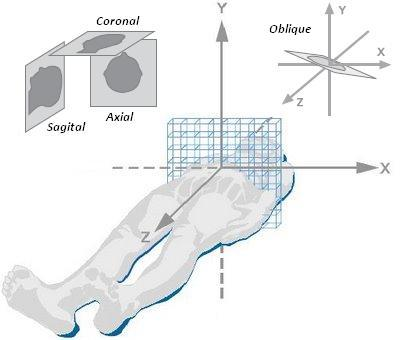
\includegraphics[scale=0.8]{Images/2_axes2.jpg}
	\caption{\textsc{mri} axis planes [sic]: coronal, sagittal and axial.}
	\small Image taken from \cite{Bean2014}.
	\label{svd-axes}
\end{figure}

As shown in Figure \ref{svd-term-fig}, \textit{volume} refers to a three-dimensional region of the scan, a \textit{point} is a single voxel in the volume, and a \textit{slice} is a cross-sectional image taken from the volume. Axial slices are taken by fixing the $z$ coordinate. Note that \textit{lines} will not be used in this thesis.

\begin{figure}[ht]
	\centering
	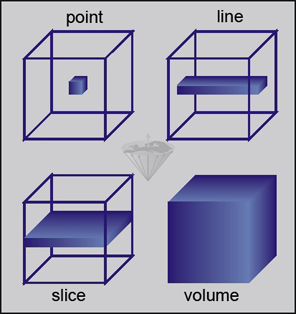
\includegraphics[scale=0.6]{Images/2_mri_volumes.jpg}
	\caption{\textsc{mri} volumes: point, line, slice and volume}
	\small Image taken from \cite{Rinck2013}.
	\label{svd-term-fig}
\end{figure}

Directional terminology in \textsc{mri} include:
\begin{itemize}
	\item \textit{anterior} and \textit{posterior}, referring to objects situated towards the front and back of the body respectively;
	\item \textit{superior} and \textit{inferior}, referring to objects situated above and below other parts of the body respectively; and
	\item \textit{interior} and \textit{exterior}, referring to objects situated closer to and further from the $x=0$ sagittal plane respectively.
\end{itemize}

\subsection*{Structure of the brain}\label{svd-brain}

% Cerebrum diagram
\begin{figure}[ht]
	\centering
	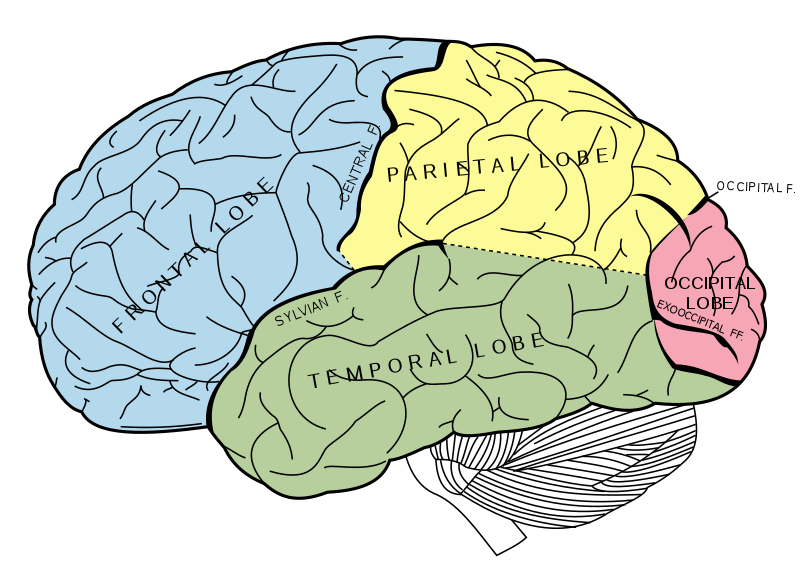
\includegraphics[width=0.7\textwidth]{Images/2_Lobes_of_the_brain_NL.png}
	\caption{The four lobes of the cerebral cortex.}
	\small Image taken from Wikimedia Commons: \url{`Gray728.svg'}.
	\label{svd-cerebrumfig}
\end{figure}

Information from throughout the body is communicated via nerves through the spinal cord to the brain. The brain is the most complex organ in the body, tasked with receiving, interpreting, and responding to nerve signals. It can be segmented into a number of regions, each responsible for different roles.

The largest region is the \textit{cerebrum}, shown in Figure \ref{svd-cerebrumfig}, which forms the outer surface of the brain. It is responsible for voluntary actions, senses, thought and memory, and is divided into two hemispheres - left and right. Each hemisphere is divided into four lobes:
 \begin{itemize}
	\item The \textit{frontal lobe}, located at the front of the cerebrum, is responsible for voluntary movement, skills and behaviours, mood, and memory.
	\item The \textit{parietal lobe}, situated posterior to the frontal lobe, is responsible for the senses, including pain, and physical and spatial awareness.
	\item The \textit{temporal lobe}, located exterior to the perietal lobe, is responsible for memory and auditory functions, including hearing and speech.
	\item The \textit{occipital lobe}, located posterior to the parietal lobe, is responsible for visual information.
\end{itemize}

The outer surface of the brain consists of a layer of neurons referred to as \textit{grey matter}. It is here that much of the brain processes occur \citep{Dafny1997}. Underneath the grey matter is a network of fibres that connects the grey matter neurons together. Collectively they form the \textit{white matter}. The grey and white matter are shown in Figure \ref{svd-greywhitefig}.

% Gray vs white matter diagram
\begin{figure}[ht]
	\centering
	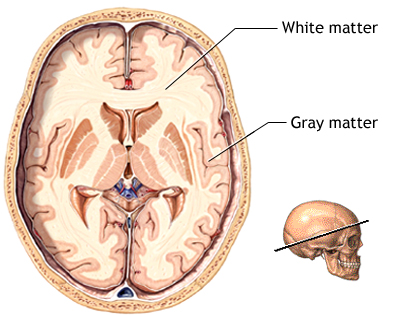
\includegraphics[width=0.6\textwidth]{Images/2_white_vs_grey.png}
	\caption{Grey matter occurs at the surface and within central structures such as the spinal cord. The white matter connects these structures together.}
	\small Image taken from \url{`https://medlineplus.gov/ency/imagepages/18117.htm'}.
	\label{svd-greywhitefig}
\end{figure}

% Basal Ganglia
\begin{figure}[ht]
	\centering
	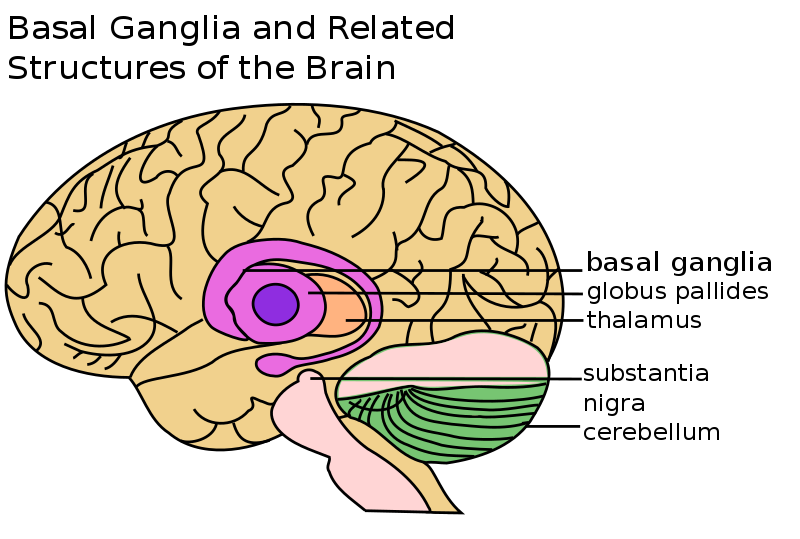
\includegraphics[width=0.7\textwidth]{Images/2_Basal_Ganglia_and_Related_Structures.png}
	\caption{The basal ganglia and other related structures.}
	\small Image taken from Wikimedia Commons: \url{`Basal_Ganglia_and_Related_Structures.svg'}.
	\label{svd-basalfig}
\end{figure}

At the centre of the brain are structures that form the \textit{basal ganglia}, shown in Figure \ref{svd-basalfig}. This region of the brain is responsible for voluntary movement and learning. Connected to this structure is the \textit{thalamus}, which is related to sensory and motor function.
%; and exhibits more numerous instances of lacunes and perivascular spaces. Two structures within the basal ganglia that are often found to have lacunes include the caudate and putamen. The thalamus is another structure that has a high frequency of lacunes, and is interconnected to the basal ganglia.

At the base of the brain lies the \textit{cerebellum}, responsible for coordination; and the \textit{brain stem}, responsible for the transmission of nerve communications. These are shown in Figure \ref{svd-basalfig}. Within the skull, the brain sits in the brain cavity filled with \textit{cerebral spinal fluid} (\textsc{csf}). This fluid can flow between the ridges at the brain's surface, filling gaps throughout the brain matter. \textsc{csf} is produced in cavities at the centre of the brain called the \textit{cerebral ventricles}.


\section{\textsc{mri}}\label{svd-MRI}

\textsc{mri} is a radiological technique that uses magnetic fields and radio waves to generate greyscale images of organs inside the body \citep{Rinck2013}. Three imaging types produced are \textit{T1-weighted}, \textit{T2-weighted} and \textit{FLuid-Attenuated Inversion Recovery} (\textsc{flair}) imaging, shown in Figure \ref{svd-t1-vs-t2}.

% Image comparisons
\begin{figure}[ht]
	\centering
	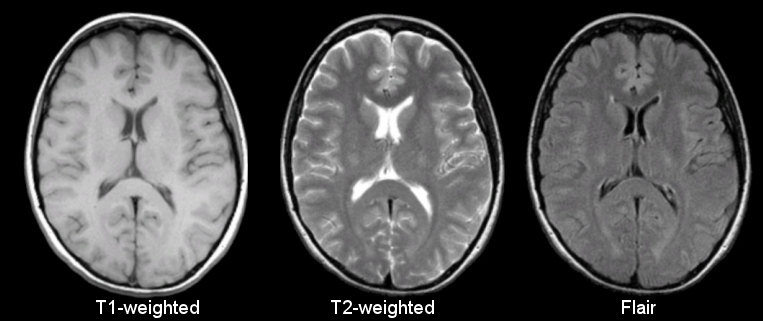
\includegraphics[width=\textwidth]{Images/2_t1_t2_flair.jpg}
	\caption{A comparison of T1, T2 and \textsc{flair} images.}
	\small Image taken from \cite{Preston2006}.
	\label{svd-t1-vs-t2}
\end{figure}

T1-weighted images are \textit{hyperintense} (bright) in regions with high fat content and are \textit{hypointense} (dark) in regions with high water content \citep{Bitar2006}. They therefore return high intensities for brain matter and low intensities for \textsc{csf}. T2-weighted images are hyperintense in regions that contain both high fat and water content \citep{Bitar2006}. This can make it easier to spot abnormalities. \textsc{flair} is an imaging sequence similar to T2-weighted imaging, excepting that \textsc{csf} remains hypointense. Abnormalities will appear bright amongst the darker \textsc{csf}, allowing for easier identification.

\section{\textsc{svd} biomarkers}\label{svd-markers}

During the analysis of \textsc{mri} scans for \textsc{svd}, there are a number of biomarkers that clinicians observe. Each of these is defined in conjunction with the \textsc{strive} criterion \citep{WardlawJ.M.2013Nsfr} shown in Figure \ref{svd-biomarkers-fig}. The schematics show a simplified representation of each biomarker for particular imaging types. Diffusion-weighted imaging (\textsc{dwi}) will not be discussed in this thesis. 

% Images of lacunes and perivascular spaces from \textsc{strive}
\begin{figure}[ht]
	\centering
	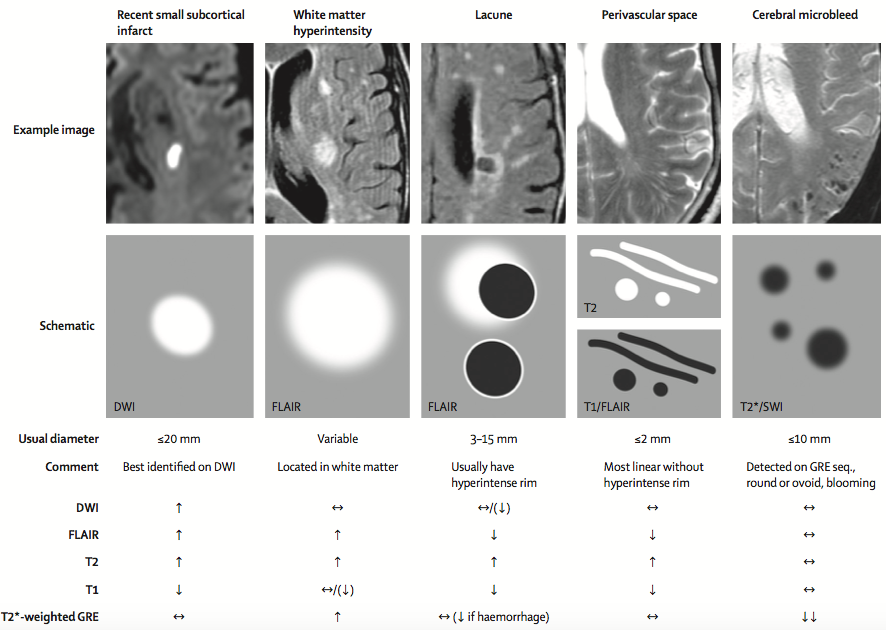
\includegraphics[width = \textwidth]{Images/2_STRIVE.png}
	\caption{\textsc{strive} criterion and \textsc{mri} examples. Up and down arrows indicate hyperintensity and hypointensity respectively. Horizontal arrows indicate structures of the same intensity.}
	\small Image taken from \cite{WardlawJ.M.2013Nsfr}.
	\label{svd-biomarkers-fig}
\end{figure}

\textit{White matter hyperintensities} (\textsc{wmh}) are regions of hyperintensity visible in T2-weighted imaging. They also appear in T1-weighted images as hypointense regions, though not as dark as \textsc{csf}. Their cause is not well understood \citep{Gouw2011}.

\textit{Lacunes} are small brain cavities. They usually appear without symptoms, and are frequently found in the scans of elderly. Their presence indicates a heightened risk of stroke and dementia \citep{BenjaminJ.Philip2018LIbN, VanDerFlierM.Wiesje2005SVDa}. In \textsc{mri}, lacunes appear round, with a diameter between 3 mm and 15 mm. They tend to give off a darker signal intensity, similar to that of \textsc{csf}, as they are filled with fluid. Lacunes have a tendency to occur in regions of white matter hyperintensity, so they will frequently have a hyperintense rim in \textsc{flair} imaging.

\textit{Perivascular spaces} are extensions of the fluid space surrounding blood vessels through the brain. They are generally microscopic but can become enlarged with age, and often appear alongside other \textsc{svd} biomarkers such as lacunes and \textsc{wmh}. Perivascular spaces also take on a signal intensity similar to \textsc{csf} as they are fluid-filled. They are found running parallel to vessels, and are generally found under 3 mm in diameter. They can be identified by appearing circular cross-sectionally and rectangular when viewed in parallel to the vessels. In some instances, perivascular spaces can become enlarged, up to 10 mm in diameter. They can be difficult to distinguish from lacunes as their signal intensities are similar.

\textit{Cerebral microbleeds} are blooming regions of microscopic bleeding, usually around 2--5 mm in diameter though they can be larger. They are not visible on T1-weighted, T2-weighted or \textsc{flair} images, and are instead found in T2*-weighted images constructed from a combination of T2-imaging and inhomogeneities in the magnetic field during scanning. 

\textit{Recent small subcortical infarcts}, are regions of recent oxygen deprivation that have resulted in cell death. They are the cause of 25\% of ischaemic (oxygen starved) strokes \citep{WardlawJ.M.2013Nsfr}. These lesions are usually less than 20 mm in diameter. 

\textit{Brain atrophy} refers to the reduction of brain matter and is not restricted to particular regions of the brain. It can be identified by the increase in \textsc{csf} volume in T1-weighted, T2-weighted and \textsc{flair} imaging.

\section{Image rating}\label{svd-rating}

Without a biopsy for confirmation, the identification of \textsc{svd} biomarkers relies on \textsc{mri} analysis. Trained observers examine \textsc{mri} volumes slice by slice and identify any lesions or points of interest. A number of rating guidelines exist in order to establish rating consistency \citep{AdamsH.H.Hieab2013RMfD, PotterGillian2015CPSV, WardlawJ.M.2013Nsfr}.

Though standardised criterion help to improve rating consistency, the appearance of lacunes and perivascular spaces are highly similar and therefore remain difficult to distinguish. As a result, manual rating is still highly inconsistent \citep{PotterGillian2015CPSV}. Additionally, the manual rating process is time consuming. \cite{Heuvel2016} report that the rating of a single scan for microbleeds takes one hour on average. Datasets with many scans can take many hours to process and the resulting identified biomarkers may not be consistent enough to warrant proper inference \citep{BenjaminJ.Philip2018LIbN, WardlawJ.M.2013Nsfr}.

In order to assist clinicians in rating quality, consistency, and speed, machine learning algorithms have been built to identify biomarkers. These algorithms can be built to work either alongside clinicians as computer-aided design (\textsc{cad}) programs \citep{Heuvel2016, Uchiyama20071554, Yokoyama2007} or as fully automated systems \citep{DouQ.2016ADoC, GhafoorianM.2017Dml3}.

%Prior to 2013, there were no official guidelines for the identification of \textsc{svd} biomarkers. There were several studies attempting to establish rating guidelines \citep{AdamsH.H.Hieab2013RMfD, PotterGillian2015CPSV}, however these methods tended to focus on specific events rather than \textsc{svd} biomarkers in general.

%In addition, much of the terminology surrounding some biomarkers was inconsistent. For instance, perivascular spaces are also frequently referred to as Virchow-Robin spaces \citep{AdamsH.H.Hieab2013RMfD, WardlawJ.M.2013Nsfr}.

%In 2013, the \textsc{strive} criterion \citep{WardlawJ.M.2013Nsfr} were established to standardise the terminology and definitions, and visual rating was conducted in conjunction with those guidelines. Though the criterion helped to improve rating consistency, the appearance of lacunes and perivascular spaces are highly similar and therefore remain difficult to distinguish. As a result, manual rating is still highly inconsistent \citep{PotterGillian2015CPSV}. 
%
%In addition, the manual rating process is also time consuming. The checking and logging of an individual scan can take over 10 minutes.

%It is only recently that machine learning algorithms have begun to improve the rating process. Dou et al. p{DouQ.2016ADoC} developed a machine learning algorithm for the detection of cerebral microbleeds. This algorithm exhibited a sensitivity of 93.16\%, with an average of 2.74 false positives per slice. 
%
%Ghafoorian et al. \citep{GhafoorianM.2017Dml3} developed a machine learning algorithm for the automated detection of lacunes. This algorithm was able to achieve a sensitivity of 97.4\%, with 0.13 false positives per slice. This algorithm will be discussed further in Section \ref{litrev-ghafoorian}.

%%%%%%%%%%%%%%%%%%%%%%%%%%%%%%%%%%%%%%%%%%%%%%%%%%%%%%%%%%%%%%%%%%%%%%%%%%

%\clearpage

\addcontentsline{toc}{chapter}{References}

\bibliographystyle{apalike}
\bibliography{bibliography.bib}

%\bibliographystyle{apacite}
%\bibliography{mybib.bib}



%\documentclass[honours,12pt,twoside]{unswthesis}

\usepackage{afterpage}
\usepackage{amsfonts}
\usepackage{amsmath}
\usepackage{amssymb}
\usepackage{amsthm}
\usepackage[english]{babel}
\usepackage{graphicx}
\usepackage{natbib}
\usepackage[utf8]{inputenc}
\usepackage{latexsym}
\usepackage{url}
\usepackage{todonotes}
\usepackage{tikz}
\usepackage{pdfpages}
\usetikzlibrary{arrows}
\usepackage{float}

\usepackage{booktabs}
\renewcommand{\arraystretch}{1.2}


%%%%%%%%%%%%%%%%%%%%%%%%%%%%%%%%%%%%%%%%%%%%%%%%%%%%%%%%%%%%%%%%%
%
%  The following are some simple LaTeX macros to give some
%  commonly used letters in funny fonts. You may need more or less of
%  these
%
\newcommand{\R}{\mathbb{R}}
\newcommand{\Q}{\mathbb{Q}}
\newcommand{\C}{\mathbb{C}}
\newcommand{\N}{\mathbb{N}}
\newcommand{\F}{\mathbb{F}}
\newcommand{\PP}{\mathbb{P}}
\newcommand{\T}{\mathbb{T}}
\newcommand{\Z}{\mathbb{Z}}
\newcommand{\B}{\mathfrak{B}}
\newcommand{\BB}{\mathcal{B}}
\newcommand{\M}{\mathfrak{M}}
\newcommand{\X}{\mathfrak{X}}
\newcommand{\Y}{\mathfrak{Y}}
\newcommand{\CC}{\mathcal{C}}
\newcommand{\E}{\mathbb{E}}
\newcommand{\cP}{\mathcal{P}}
\newcommand{\cS}{\mathcal{S}}
\newcommand{\A}{\mathcal{A}}
\newcommand{\ZZ}{\mathcal{Z}}

%%%%%%%%%%%%%%%%%%%%%%%%%%%%%%%%%%%%%%%%%%%%%%%%%%%%%%%%%%%%%%%%%%%%%
%
% The following are much more esoteric commands that I have left in
% so that this file still processes. Use or delete as you see fit
%
\newcommand{\bv}[1]{\mbox{BV($#1$)}}
\newcommand{\comb}[2]{\left(\!\!\!\begin{array}{c}#1\\#2\end{array}\!\!\!\right)
}
\newcommand{\Lat}{{\rm Lat}}
\newcommand{\var}{\mathop{\rm var}}
\newcommand{\Pt}{{\mathcal P}}
\def\tr(#1){{\rm trace}(#1)}
\def\Exp(#1){{\mathbb E}(#1)}
\def\Exps(#1){{\mathbb E}\sparen(#1)}
\newcommand{\floor}[1]{\left\lfloor #1 \right\rfloor}
\newcommand{\ceil}[1]{\left\lceil #1 \right\rceil}
\newcommand{\hatt}[1]{\widehat #1}
\newcommand{\modeq}[3]{#1 \equiv #2 \,(\text{mod}\, #3)}
\newcommand{\rmod}{\,\mathrm{mod}\,}
\newcommand{\p}{\hphantom{+}}
\newcommand{\vect}[1]{\mbox{\boldmath $ #1 $}}
\newcommand{\reff}[2]{\ref{#1}.\ref{#2}}
\newcommand{\psum}[2]{\sum_{#1}^{#2}\!\!\!'\,\,}
\newcommand{\bin}[2]{\left( \begin{array}{@{}c@{}}
				#1 \\ #2
			\end{array}\right)	}
%
%  Macros - some of these are in plain TeX (gasp!)
%
\newcommand{\be}{($\beta$)}
\newcommand{\eqp}{\mathrel{{=}_p}}
\newcommand{\ltp}{\mathrel{{\prec}_p}}
\newcommand{\lep}{\mathrel{{\preceq}_p}}
\def\brack#1{\left \{ #1 \right \}}
\def\bul{$\bullet$\ }
\def\cl{{\rm cl}}
\let\del=\partial
\def\enditem{\par\smallskip\noindent}
\def\implies{\Rightarrow}
\def\inpr#1,#2{\t \hbox{\langle #1 , #2 \rangle} \t}
\def\ip<#1,#2>{\langle #1,#2 \rangle}
\def\lp{\ell^p}
\def\maxb#1{\max \brack{#1}}
\def\minb#1{\min \brack{#1}}
\def\mod#1{\left \vert #1 \right \vert}
\def\norm#1{\left \Vert #1 \right \Vert}
\def\paren(#1){\left( #1 \right)}
\def\qed{\hfill \hbox{$\Box$} \smallskip}
\def\sbrack#1{\Bigl \{ #1 \Bigr \} }
\def\ssbrack#1{ \{ #1 \} }
\def\smod#1{\Bigl \vert #1 \Bigr \vert}
\def\smmod#1{\bigl \vert #1 \bigr \vert}
\def\ssmod#1{\vert #1 \vert}
\def\sspmod#1{\vert\, #1 \, \vert}
\def\snorm#1{\Bigl \Vert #1 \Bigr \Vert}
\def\ssnorm#1{\Vert #1 \Vert}
\def\sparen(#1){\Bigl ( #1 \Bigr )}

\newcommand\blankpage{%
    \null
    \thispagestyle{empty}%
    \addtocounter{page}{-1}%
    \newpage}
    
%%%%%%%%%%%%%%%%%%%%%%%%%%%%%%%%%%%%%%%%%%%%%%%%%%%%%%%%%%%%%%
%
% These environments allow you to get nice numbered headings
%  for your Theorems, Definitions etc.  
%
%  Environments
%
%%%%%%%%%%%%%%%%%%%%%%%%%%%%%%%

\newtheorem{theorem}{Theorem}[section]
\newtheorem{lemma}[theorem]{Lemma}
\newtheorem{proposition}[theorem]{Proposition}
\newtheorem{corollary}[theorem]{Corollary}
\newtheorem{conjecture}[theorem]{Conjecture}
\newtheorem{definition}[theorem]{Definition}
\newtheorem{example}{Example}
\newtheorem{remark}[theorem]{Remark}
\newtheorem{question}[theorem]{Question}
\newtheorem{notation}[theorem]{Notation}
\numberwithin{equation}{section}

%\begin{document}

\chapter{Neural networks}\label{neuralNets-intro}

This chapter outlines the structure and workings of basic neural network models. Those who have a basic understanding of neural networks and wish to avoid the details surrounding model structure and minimisation algorithms can proceed to Chapter \ref{convnets} for an overview of convolutional neural networks and Chapter \ref{litrev} for existing lacune model attempts.

% - Basic neural networks theory + perceptron
% - Loss functions
% - Minimisation functions
% 
% - Convolutional neural networks overview
% - Convolution layer
% - ReLU
% - Pooling
% - Fully connected layers
% 
% - 3D CNNs overview

Neural networks have become increasingly popular with advances in computing power and the availability of large data sets \cite{Goodfellow-et-al-2016}. They have been proven successful with \textsc{mri} discrimination tasks \cite{DouQ.2016ADoC, Yokoyama2007} and image classification tasks \cite{AlexNet2012, GoogLeNet2015, HeKaiming2015DDiR}. In some instances, neural networks have exhibited a higher image recognition accuracy than humans \cite{HeKaiming2015DDiR}.

The construction of neural networks has to be conducted with care. The resulting models are difficult to interpret and prone to overfitting. We now discuss the underlying structure of neural networks, loss minimisation, and techniques to avoid overfitting the data.

\section{Basic structure}\label{nnets-structure}

The structure of neural networks can be compared to that of neurons in the brain. Each brain cell receives a signal, conducts a small amount of processing, and passes the resulting signal to the next cell. Decisions made by the brain are the result of many neurons processing information in sequence. Neural networks adopt a similar structure. Individual nodes receive variables, apply a transformation, and pass the result to the next node. For this reason, the nodes are referred to as \textit{neurons}.

The structure of a neural network neuron is shown in Figure \ref{nnet-neuronfig}. Let $\mathbf{x} = (x_1, x_2, \ldots, x_n)^\intercal$ be a vector of $n$ input variables. Let $\mathbf{w} = (w_1, \ldots, w_n)^\intercal$ be a vector of weights. Let $b$ be an additional \textit{bias} variable. This bias is not to be confused with statistical bias and is included to provide the neuron with a constant term. The output of a single neuron is given by
\[
	a = \sigma(\mathbf{w}\cdot\mathbf{x} + b),
\]
where $\sigma(\cdot)$ is an \textit{activation function} and $a$ is an \textit{activation value}.



% Neuron structure diagram
\begin{figure}
\centering
\tikzset{every picture/.style={line width=0.75pt}} %set default line width to 0.75pt        

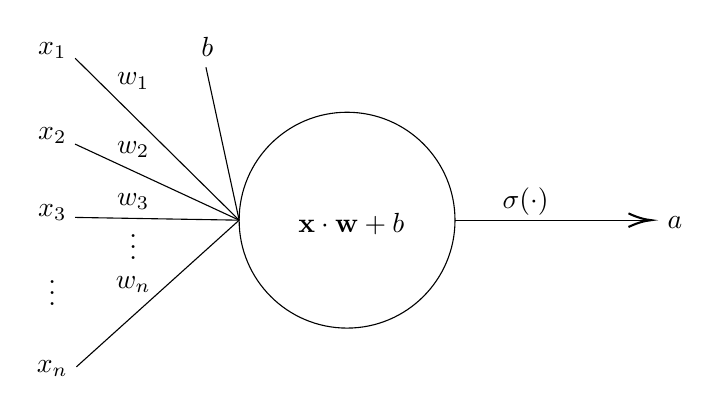
\begin{tikzpicture}[x=0.75pt,y=0.75pt,yscale=-1,xscale=1]
%uncomment if require: \path (0,300); %set diagram left start at 0, and has height of 300

%Shape: Circle [id:dp7806506925261892] 
\draw   (270,154) .. controls (270,125.28) and (293.28,102) .. (322,102) .. controls (350.72,102) and (374,125.28) .. (374,154) .. controls (374,182.72) and (350.72,206) .. (322,206) .. controls (293.28,206) and (270,182.72) .. (270,154) -- cycle ;
%Straight Lines [id:da48045113953293783] 
\draw    (191,76) -- (270,154) ;


%Straight Lines [id:da20730706323067383] 
\draw    (190.92,117.33) -- (270,154) ;


%Straight Lines [id:da19390293965519045] 
\draw    (191.59,224.67) -- (270,154) ;


%Straight Lines [id:da5499170807272789] 
\draw    (374,154) -- (466.51,154) ;
\draw [shift={(468.51,154)}, rotate = 180] [color={rgb, 255:red, 0; green, 0; blue, 0 }  ][line width=0.75]    (10.93,-3.29) .. controls (6.95,-1.4) and (3.31,-0.3) .. (0,0) .. controls (3.31,0.3) and (6.95,1.4) .. (10.93,3.29)   ;

%Straight Lines [id:da7426731370805287] 
\draw    (270,154) -- (190.92,152.67) ;


%Straight Lines [id:da35133187079282135] 
\draw    (254,80.33) -- (270,154) ;



% Text Node
\draw (324,156) node   {$\mathbf{x} \cdot \mathbf{w} +b$};
% Text Node
\draw (180,72.33) node   {$x_{1}$};
% Text Node
\draw (180,113.33) node   {$x_{2}$};
% Text Node
\draw (180,185) node   {$\vdots $};
% Text Node
\draw (180,225.33) node   {$x_{n}$};
% Text Node
\draw (180,150.33) node   {$x_{3}$};
% Text Node
\draw (219,87) node   {$w_{1}$};
% Text Node
\draw (219,120) node   {$w_{2}$};
% Text Node
\draw (219,145) node   {$w_{3}$};
% Text Node
\draw (219,185) node   {$w_{n}$};
% Text Node
\draw (219,163) node   {$\vdots $};
% Text Node
\draw (254.67,70.33) node   {$b$};
% Text Node
\draw (408,145) node   {$\sigma ( \cdot )$};
% Text Node
\draw (480,155) node   {$a$};


\end{tikzpicture}
\caption{Neuron structure.}
\label{nnet-neuronfig}
\end{figure}






%% Diagram of single neuron
%\begin{figure}[ht]
%	\centering
%	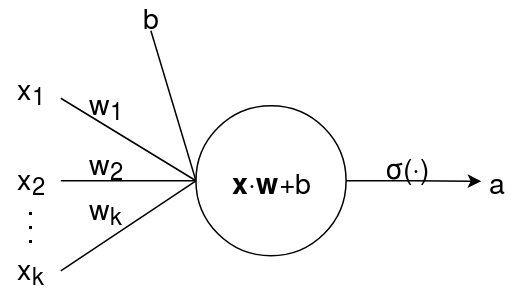
\includegraphics[scale=0.5]{Images/3_neuron.png}
%	\caption{Neuron structure.}
%	\label{nnet-neuronfig}
%\end{figure}

A large number of these neurons can be arranged to form a neural network. The generated outputs of these neurons can be fed as inputs into later neurons. Basic neural networks arrange a number of these neurons into layers, as shown in Figure \ref{nnet-structurefig}. The first layer is an input layer, where data is fed into the model. Each neuron in this first layer represents a variable. The last layer is an output layer which generates the final result. The central layers, which conduct most of the processing, are known as \textit{hidden layers}.

% Diagram of basic neural network structure. Input, 1 hidden layer and series of output layers
%\begin{figure}[ht]
%	\centering
%	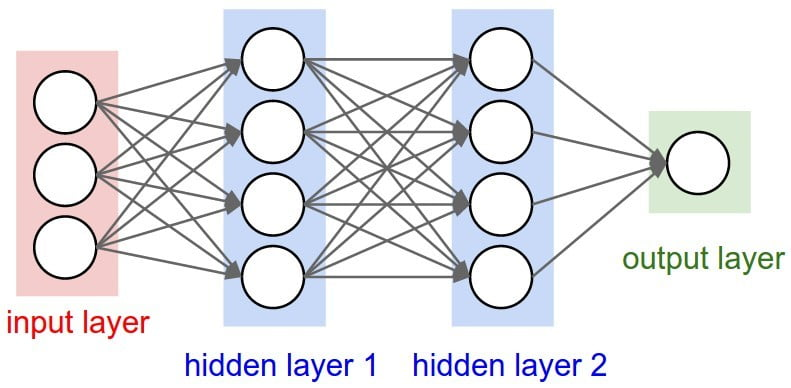
\includegraphics[width=\textwidth]{Images/3_nnet_structure.jpg}
%	\caption{Basic neural network structure.}
%	\small Image taken from \url{`https://www.digitaltrends.com/cool-tech/what-is-an-artificial-neural-network/'}
%	\label{nnet-structurefig}
%\end{figure}
\begin{figure}
\centering
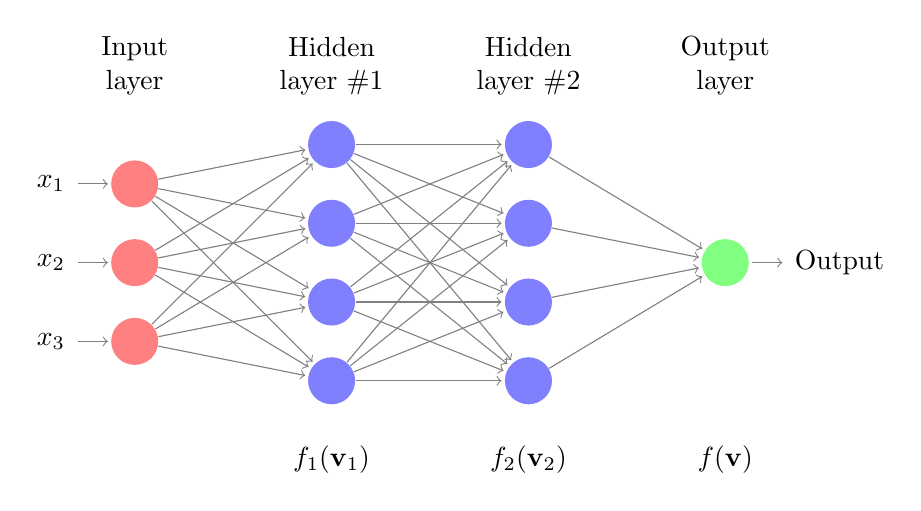
\begin{tikzpicture}[shorten >=1pt,->,draw=black!50, node distance=\layersep]
    \tikzstyle{every pin edge}=[<-,shorten <=1pt]
    \tikzstyle{neuron}=[circle,fill=black!25,minimum size=17pt,inner sep=0pt]
    \tikzstyle{input neuron}=[neuron, fill=red!50];
    \tikzstyle{output neuron}=[neuron, fill=green!50];
    \tikzstyle{hidden neuron}=[neuron, fill=blue!50];
    \tikzstyle{annot} = [text width=4em, text centered]
	\def\layersep{2.5cm}
	
    % Draw the input layer nodes
    \foreach \name / \y in {1,...,3}
    % This is the same as writing \foreach \name / \y in {1/1,2/2,3/3,4/4}
        \node[input neuron, pin=left:$x_\y$] (I-\name) at (0,-\y) {};

    % Draw the hidden layer1 nodes
    \foreach \name / \y in {1,...,4}
        \path[yshift=0.5cm]
            node[hidden neuron] (Ha-\name) at (\layersep,-\y cm) {};
            
    % Draw the hidden layer2 nodes
    \foreach \name / \y in {1,...,4}
        \path[yshift=0.5cm]
            node[hidden neuron] (Hb-\name) at (2*\layersep,-\y cm) {};

    % Draw the output layer node
    \node[output neuron,pin={[pin edge={->}]right:Output}] (O) at (3*\layersep, -2) {};

    % Connect every node in the input layer with every node in the
    % hidden layer.
    \foreach \source in {1,...,3}
        \foreach \dest in {1,...,4}
            \path (I-\source) edge (Ha-\dest);
            
    % Connect every node in the hidden layer 1 with every node in
    % hidden layer 2.
    \foreach \source in {1,...,4}
        \foreach \dest in {1,...,4}
            \path (Ha-\source) edge (Hb-\dest);

    % Connect every node in the hidden layer with the output layer
    \foreach \source in {1,...,4}
        \path (Hb-\source) edge (O);

    % Annotate the layers
    \node[annot,above of=Ha-1, node distance=1cm] (hla) {Hidden layer \#1};
    \node[annot,above of=Hb-1, node distance=1cm] (hlb) {Hidden layer \#2};
    \node[annot,left of=hla] {Input layer};
    \node[annot,right of=hlb] {Output layer};
    
    \node[annot,below of=Ha-4, node distance=1cm] (fa) {$f_1(\mathbf{v}_1)$};
    \node[annot,below of=Hb-4, node distance=1cm] (fb) {$f_2(\mathbf{v}_2)$};
    \node[annot,right of=fb, node distance=\layersep] (fo) {$f(\mathbf{v})$};

\end{tikzpicture}
\caption{Basic neural network structure. Each hidden neuron (blue) and the output neuron (green) has the structure shown in Figure \ref{nnet-neuronfig}. For simplicity, the weights and biases have been hidden.}
\label{nnet-structurefig}
\end{figure}

Let the weights and biases of layer $\ell$ be $\mathbf{v}_\ell$ and let the output of hidden layer $\ell$ be $f_\ell(\mathbf{v}_\ell)$. Then the output of the whole network is
\[
	f(\mathbf{v}) = f_L(\mathbf{v}_L) \circ f_{L-1}(\mathbf{v}_{L-1}) \circ \ldots \circ f_1(\mathbf{v}_1).
\]

All the weights $W$ and biases $B$ of the network are chosen such that they minimise some \textit{cost function} $C(W,B)$ with respect to $(W,B)$. However, since the number of variables can be very large, it is not always feasible to analytically minimise $C(W,B)$.

We can instead approximate this minimisation via the Gradient-Descent algorithm (see Section \ref{nnets-graddesc}). This algorithm is run until the cost function falls within some tolerance $\tau$, or reaches the maximum number of iterations $n_T$.

\section{Notation}\label{nnets-not}

\todo[inline]{Restructure notation like a glossary. Two columns, notation on left and definition on right.}

Let $\mathbf{w}^\ell_j$ to be the vector of weights used to compute the $j$-th neuron of the $\ell$-th layer, where $w_{ji}^\ell$ is the weight attributed to the $i$-th neuron of the $(\ell-1)$-th layer.

Let $b_j^\ell$ be the bias of the $j$-th neuron in the $\ell$-th layer.

Let $\mathbf{a}^\ell$ be the vector of activation values (outputs) for the $\ell$-th layer, where $a_j^\ell$ is the activation value of the $j$-th neuron of that layer. Set $z_j^\ell := \mathbf{w}_j^\ell\cdot \mathbf{a}^{\ell-1} + b_j^\ell= \sum_k w_{jk}^\ell a_k^{\ell-1} + b_j^\ell$ to be the values calculated before activation, and $\mathbf{z}^\ell$ to be the vector of $z_j^\ell$ for the $\ell$-th layer. Set $Z$ to be the set of all $z_j^\ell$ in the whole network. Let $L$ be the number of layers in the network so that $\mathbf{a}^L$ is the vector of activation values of the final output layer. Let $X = \{\mathbf{x}_1, \mathbf{x}_2, \ldots, \mathbf{x}_n\}$ be the set of $n$ training inputs. Let the responses be $Y = \{\mathbf{y}_1, \mathbf{y}_2, \ldots, \mathbf{y}_n\}$, with $y_{ij}$ the $j$-th variable of $\mathbf{y}_i$. Let $W$ and $B$ be the sets of all weights and biases as before. Let $\eta$ be the learning rate of the network. 

\section{Activation functions}\label{nnets-act}

Activation functions, denoted by $\sigma(\cdot)$, are applied just before neuron output. Without these functions, the network can be reduced to a linear combination of inputs. Activation functions serve to introduce nonlinearity into the model.

The simplest neuron type is called the \textit{perceptron}. In this neuron, the activation function is the step function,
\[
	x_i \in \{0,1\} \text{ and } \sigma(z) = \begin{cases}
		1 & z > 0 \\
		0 & z \le 0
	\end{cases}.
\]

To allow for continuous outputs, other common activation functions include the sigmoid function
\[
	\sigma(z) = \dfrac{1}{1+e^{-z}},
\]
and hyperbolic tan function,
\[
	\sigma(z) = \tanh(z),
\]
which are smooth approximations to a step activation function.

The Rectified Linear Unit (ReLU) activation is given by,
\[
	\sigma(z) = \max(0, z),
\]
which allows for some neurons to output 0 and be essentially deactivated.

A common activation function for the final layer is the softmax function,
\[
	\sigma(z_j) = \dfrac{e^{z_j}}{\sum_ke^{z_k}},
\]
as the output takes the form of a probability distribution.


\section{Cost functions}\label{nnets-cost}

Weights and biases are chosen such that they approximately minimise some cost function. To use the gradient descent algorithm (see Section \ref{nnets-graddesc}) to minimise cost, Nielson \cite{Nielson2015} describes two requirements. The first requirement is that the cost $C_X(\cdot)$ accrued from all samples $X$ equals the mean of costs accrued from $n$ distinct subsamples of $X$, denoted by $X_i$,
\[
	C_X(W, B) = \dfrac{1}{n}\sum_{i=1}^n C_{X_i}(W,B).
\]

The second requirement is that the cost is independent of $\mathbf{a}^\ell$ for all $\ell < L$. There are a number of cost functions in frequent use, and the choice of cost function is dependent on the context of the problem. A common cost function for regression is the quadratic cost, or Mean Squared Error (\textsc{mse}) cost. Denote $\|\cdot\|$ to be the Euclidean norm. The \textsc{mse} cost function is given by
\[
	C(W,B) = \dfrac{1}{2n}\sum_{i=1}^n||\mathbf{a}^L(\mathbf{x}_i,W,B) - \mathbf{y}_i ||^2.
\]
This form is convenient for backpropagation (see Section \ref{nnets-backprop}) as it has an efficiently computable gradient,
\[
	\nabla_aC = \dfrac{1}{n}\sum_{i=1}^n||\mathbf{a}^L(\mathbf{x}_i,W,B) - \mathbf{y}_i ||.
\]
In using quadratic cost, if the amount of error is large, the learning rate is low.

The most common cost function for classification tasks is cross entropy, given by
\[
	C(W,B) = -\dfrac{1}{n}\sum_{i=1}^n\sum_j\big[y_{ij}\log\big(a_j^L(\mathbf{x}_i,W,B)\big) + (1 - y_{ij})\log\big( (1 - a_j^L(\mathbf{x}_i,W,B))\big)\big],
\]
with gradient
\[
	\nabla_aC = \dfrac{1}{n}\sum_{i=1}^n\sum_j\dfrac{a_j^L(\mathbf{x}_i,W,B) - y_{ij}}{a_j^L(\mathbf{x}_i,W,B)(1-a_j^L(\mathbf{x}_i,W,B))}.
\]
Unlike the quadratic cost, when the error is high, the learning rate is also high.

%Cost functions can include: the quadratic (simple), cross-entropy, regularisation (L1, L2, dropout, artificial expansion of training data).
%In using cross-entropy, the learning rate of the weight is controlled by the amount of error. This is unlike the quadratic cost function, which has a very slow learning rate when there is high error.
%Changing these can improve a model.
%Other improvements made by making better initialisations of weights, and better heuristics to choose hyper-parameters.

\section{Gradient descent}\label{nnets-graddesc}

Weights and biases are chosen to minimise the cost function. Analytically minimising the cost function is possible, however the large number of variables makes this process slow, having time complexity $O(n^3)$ \cite{Marquardt1963}. To improve computation speed, the weights are instead estimated using the Gradient Descent algorithm.

Gradient Descent works by considering the gradient of the cost given the current weights and biases \cite{Nielson2015}. The algorithm shifts the weights and biases by a small amount such that the cost will decrease. The amount that the values shift by is referred to as the learning rate, denoted $\eta$ as before.

Let $N$ be a positive integer. For all weights and biases denoted $\mathbf{v}$, the change in cost $C(\mathbf{v})$ is given by the \textit{Total Differential Approximation},
\begin{align*}
	\Delta C(\mathbf{v}) & \approx \dfrac{\partial C}{\partial v_1}\Delta v_1 + \dfrac{\partial C}{\partial v_2}\Delta v_2 + \cdots + \dfrac{\partial C}{\partial v_N}\Delta v_N\\
	& = \nabla C(\mathbf{v})\cdot \Delta \mathbf{v},
\end{align*}
where $\nabla C(\mathbf{v}) = \Big(\dfrac{\partial C}{\partial v_1}, \dfrac{\partial C}{\partial v_2},\ldots, \dfrac{\partial C}{\partial v_N}\Big)$.

We define $\mathbf{v}'$ to be the updated value of $\mathbf{v}$. We update $\mathbf{v}'$ inductively such that the cost decreases by an amount proportional to $\eta$.

The next values of $\mathbf{v}$ are chosen such that the cost will decrease by an amount controlled by $\eta$, such that
\[
	\Delta\mathbf{v} = -\eta \nabla C(\mathbf{v}), \quad \text{ where }\eta > 0.
\]
By substitution, we can write
\[
	\Delta C(\mathbf{v}) \approx -\eta \|\nabla C(\mathbf{v})\|^2 \le 0,
\]
where $\|\cdot\|$ is the Euclidean norm.

Thus if $\mathbf{v}' := \mathbf{v} - \eta \nabla C(\mathbf{v})$, the cost will decrease.

In training a neural network, the size of the shift can be set to $\|\Delta\mathbf{v}\| = \varepsilon$, for some $\varepsilon > 0$. It can be shown that the $\Delta\mathbf{v}$ which gives the greatest decrease in $C(\mathbf{v})$ is a function of $\varepsilon$ and $\nabla C$ \cite{Nielson2015}.

\begin{proposition}\label{nnets-graddescminproof}
	Let $\varepsilon > 0$ and suppose the size of the shift is constrained such that $\|\Delta\mathbf{v}\| = \varepsilon$. Then $\nabla C \cdot \Delta\mathbf{v}$ is minimised by $\Delta\mathbf{v} = -\eta\nabla C$, where $\eta = \dfrac{\varepsilon}{\|\nabla C\|}$.
\end{proposition}

\begin{proof}
	Using the Cauchy-Schwarz Inequality,
	\[
			|\nabla C\cdot\Delta\mathbf{v}| \le \|\nabla C\|\cdot\|\Delta\mathbf{v}\|.
	\]
	Then the minimum is given by, \begin{align*}
		\min(\nabla C\cdot\Delta\mathbf{v}) & = -\|\nabla C\|\times\|\Delta\mathbf{v}\| \\
		& = -\varepsilon\|\nabla C\| \\
		& = -\dfrac{\varepsilon\|\nabla C\|^2}{\|\nabla C\|} \\
		& = -\dfrac{\varepsilon\nabla C\cdot\nabla C}{\|\nabla C\|}.
	\end{align*}
	Then by equating the coefficients of $\nabla C$,
	\begin{align*}
		\operatorname*{arg\,min}_{\Delta\mathbf{v}}(\nabla C\cdot\Delta\mathbf{v}) & = -\dfrac{\varepsilon\nabla C}{\|\nabla C\|} \\
		& = -\eta\nabla C,\quad\text{ where }\eta = \dfrac{\varepsilon}{\|\nabla C\|}.
	\end{align*}
\end{proof}

As gradient descent moves the coefficients in the direction of the steepest negative gradient, it assumes that the starting values are close enough to the global minimum to converge. If this assumption is not satistifed, the algorithm will instead converge to the local minimum. However, it is not possible to confirm whether the weights are converging to the global minimum or not.

%To address this, it is commonplace to initialise the weights randomly.
%
%A common distribution for initialising weights is the truncated normal distribution, which has the shape of the normal distribution $\mathcal{N}(\mu, \sigma^2)$, but is bounded such that $X\in(a,b),-\infty\le a < b\le \infty$.

As the updated weights and biases rely on the gradient, it should be noted that these gradients are then required to be significantly different from zero. When this is not the case, we have what is called the Vanishing Gradient Problem, which is discussed further in section \ref{nnet-vanishinggradprob}.

\subsection*{Stochastic gradient descent}\label{nnets-stochgraddesc}

As the neural network has a very large number of weights, gradient descent is a highly computationally intensive algorithm. To improve training time, Stochastic Gradient Descent is a popular alternative, shown to have a time complexity of $O(n)$ \cite{Robbins1951}. This algorithm improves learning speed by randomly selecting a small number of training inputs to learn from, referred to as a \textit{batch}. After training has been completed for that batch, another batch of training inputs is randomly selected, and the process repeats. When all training batches have been used, it is said that an \textit{epoch} of training has been completed.

In this manner, a relatively small number of samples is used for each weight adjustment. This drastically increases training speed, while still utilising all the information provided by the whole set of samples by the end of training time.

\subsection*{Adam optimiser}\label{nnets-adam}

The stochastic gradient algorithm maintains one learning rate for all of the weights in the network. The Adam Optimiser alters this algorithm by storing different learning rates for each of the parameters. 

%
%We attempt to choose weights and biases that will minimise the cost function. As we cannot use calculus, we must estimate - by gradient descent. Move all the estimates a little, in the direction of decrease. The amount of movement is dependent on a learning rate parameter.
%
%This takes a long time with all inputs. Stochastic gradient descent instead randomly choosing $m$ training inputs, known as a mini-batch. It trains with the mini-batch, then rechooses $m$ different, unused inputs, re-trains, etc. When there are no more inputs to choose from, the algorithm has completed an 'epoch' of training.
%
%Backpropagation: gradient of the cost function. 

\subsection*{Learning rate}\label{nnets-learningrate}

The learning rate, given by $\eta$, controls the adjustment of weights during training. As in Section \ref{nnets-graddesc}, the change in gradients, $\Delta\mathbf{v} = -\eta\nabla C$, moves the weights in the direction of the steepest negative gradient. $\eta$ then controls the magnitude of the movement.

The size of $\eta$ controls how quickly the model learns. If $\eta$ is too small, training will take a long time. If $\eta$ is too large, the model may move the weights too far, and the values of $\mathbf{v}$ will move past the local minimum.

To aid in efficient training, learning rates can be adjusted throughout. At the start of training, it can be beneficial to have a higher learning rate. This allows the weights to move closer to the local minimum much faster. At later epochs, a smaller learning rate will allow for fine tuning of the weights, ensuring precision. A common technique is to lower the learning rate only when validation accuracy drops.

\section{Backpropagation}\label{nnets-backprop}

During gradient descent, it is necessary to calculate the gradient of the cost function. This is done through backpropagation. This algorithm determines $\dfrac{\partial C}{\partial z}$, then relates those values to the rates of interest, $\dfrac{\partial C}{\partial W}$ and $\dfrac{\partial C}{\partial B}$. To describe the algorithm, we first need to derive some results.

% http://neuralnetworksanddeeplearning.com/chap2.html

\begin{proposition}
	The error of the jth neuron of the final output layer is
	\[
		\delta_j^L = \dfrac{\partial C}{\partial a_j^L}\sigma'(z_j^L).
	\]
	This can be expressed in the matrix form,
	\[
		\delta^L = \Sigma'(\mathbf{z}^L)\nabla_aC,
	\]
where $\Sigma'(\cdot)$ is a matrix where the $j$-th diagonal entry is $\sigma'(z_j^L)$ and all non-diagonal entries are 0.
\end{proposition}

\begin{proof}
	\begin{align*}
		\delta_j^L & = \dfrac{\partial C}{\partial z_j^L} \\
		& = \sum_k\dfrac{\partial C}{\partial a_k^L}\dfrac{\partial a_k^L}{\partial z_j^L} \\
		& = \dfrac{\partial C}{\partial a_j^L}\dfrac{\partial a_j^L}{\partial z_j^L}\text{, as }z_j^L\text{ is only a function of }a_k^L\text{ for }k = j \\
		& = \dfrac{\partial C}{\partial a_j^L}\sigma'(z_j^L).
	\end{align*}
\end{proof}

\begin{proposition}
	The error $\delta^\ell_j$ can be written in terms of the errors in the next layer, 
	\begin{align*}
		\delta_j^\ell & = \sum_k\delta_k^{\ell+1}w_{kj}^{\ell+1}\sigma'(z_j^\ell).
	\end{align*}
\end{proposition}

\begin{proof}
	Using the chain rule,
	\begin{align*}
		\delta_j^\ell & = \dfrac{\partial C}{\partial z_j^\ell} \\
		& = \sum_k\dfrac{\partial C}{\partial z_k^{\ell+1}}\dfrac{\partial z_k^{\ell+1}}{\partial z_j^\ell} \\
		& = \sum_k\delta_k^{\ell+1}\dfrac{\partial z_k^{\ell+1}}{\partial z_j^\ell}.
	\end{align*}
	Then as $\dfrac{\partial z_k^{\ell+1}}{\partial z_j^\ell} = \dfrac{\partial}{\partial z_j^\ell}(\mathbf{w}_k^{\ell+1}\cdot\sigma(\mathbf{z}^\ell) + b_k^{\ell+1}) = w_{kj}^{\ell+1}\sigma'(z_j^\ell)$,
	\begin{align*}
		\delta_j^\ell & = \sum_k\delta_k^{\ell+1}w_{kj}^{\ell+1}\sigma'(z_j^\ell).
	\end{align*}
\end{proof}


Together, the errors of layer $l$ can be written
\begin{align*}
	\delta^\ell & = \Sigma'(\mathbf{z}^\ell)(w^{\ell+1})^\intercal\delta^{\ell+1} \\
	& = \Sigma'(\mathbf{z}^\ell)(w^{\ell+1})^\intercal\ldots\Sigma'(\mathbf{z}^{L-1})(w^L)^\intercal\Sigma'(\mathbf{z}^L)\nabla_aC.
\end{align*}

\begin{proposition}
	The error $\delta_j^\ell$ is equivalent to the rate of change in cost with respect to the bias, so that
	\[
		\delta_j^\ell = \dfrac{\partial C}{\partial b_j^\ell}.
	\]
\end{proposition}
\begin{proof}
	By definition,
	\[
		\delta_j^\ell = \dfrac{\partial C}{\partial z_j^\ell}.
	\]
	Then by the chain rule,
	\[
		\delta_j^\ell = \sum_k\dfrac{\partial C}{\partial b_k^\ell}\dfrac{\partial b_k^\ell}{\partial z_j^\ell}.
	\]
	Then as $z_j^\ell$ is only a function of $b_k^\ell$ for $j = k$,
	\begin{align*}
		\delta_j^\ell & = \dfrac{\partial C}{\partial b_j^\ell}\dfrac{\partial b_j^\ell}{\partial z_j^\ell} \\
		& = \dfrac{\partial C}{\partial b_j^\ell}.
	\end{align*}
\end{proof}

\begin{proposition}
	The rate of change in cost with respect to any single weight value is given by
	\[
		\dfrac{\partial C}{\partial w_{jk}^\ell} = a_k^{\ell-1}\delta_j^\ell.
	\]
\end{proposition}
\begin{proof}
	By definition,
	\begin{align*}
		z_k^\ell & = \mathbf{w}_k^\ell\cdot\mathbf{a}^{\ell-1} + b_k^\ell \\
		& = \sum_jw_{kj}^\ell a_j^{\ell-1} + b_k^\ell.
	\end{align*}
	Then differentiating with respect to some weight $w_{km}^\ell$,
	\[
		\dfrac{\partial z_k^\ell}{\partial w_{km}^\ell} = a_m^{\ell-1}.
	\]
	Then using the Chain Rule,
	\begin{align*}	
		\dfrac{\partial C}{\partial w_{jk}^\ell} & = \dfrac{\partial C}{\partial z_j^\ell}\dfrac{\partial z_j^\ell}{\partial w_{jk}^\ell} \\
		& = \delta_j^\ell a_k^{\ell-1}.
	\end{align*}
\end{proof}


Using these equations, the backpropagation algorithm runs as follows:
\begin{enumerate}
	\item \textbf{Inputs}. Enter observations $x$ to retrieve $\mathbf{a}^1$.
	\item \textbf{Feedforward}. Compute the $\mathbf{z}^\ell = \mathbf{w}^\ell\mathbf{a}^{\ell-1} + \mathbf{b}^\ell$ for each $l = 2, 3,\ldots,L$.
	\item \textbf{Output error}. Compute $\delta^L = \Sigma'(\mathbf{z}^L)\nabla_aC$.
	\item \textbf{Backpropagation}. For $\ell = L-1, \ldots, 2$, compute $\delta^\ell =  \Sigma'(\mathbf{z}^\ell)(w^{\ell+1})^\intercal\delta^{\ell+1}$.
	\item \textbf{Gradients}. Compute $\dfrac{\partial C}{\partial b_j^\ell} = \delta_j^\ell$ and $\dfrac{\partial C}{\partial w_{jk}^\ell} = a_k^{\ell-1}\delta_j^\ell$.
\end{enumerate}


\subsection*{Vanishing gradient problem}\label{nnet-vanishinggradprob}
We note that the error, $\delta^\ell$, is dependent on the gradient of the activation function. If the gradient of the activation is close to 0, then both the error detected and learning rate also become close to 0.

\noindent For the sigmoid activation function,
\[
	\sigma '(z) = e^{-z}(1+e^{-z})^{-2}.
\]
For the tanh activation function,
\[
	\sigma '(z) = 1-\tanh^2(z).
\]
For both the sigmoid and tanh activations, the limit as $z\rightarrow\pm\infty$ yields 
\[
	\lim_{z\rightarrow\pm\infty}\sigma '(z)= 0.
\]
For the sigmoid and tanh activation functions, very large or very small $z_j^\ell$ will have near zero gradients. In this scenario, the training of weights and biases shift by smaller and smaller increments, so that further training does not improve the model over time.

A common alternative to these is the ReLU activation function. This activation has gradient
\[
	\sigma '(z) = \begin{cases}
		1 & z > 0 \\
		0 & z < 0
	\end{cases}.
\]
% Paper: https://www.utc.fr/~bordesan/dokuwiki/_media/en/glorot10nipsworkshop.pdf
Neurons that are active will have a constant gradient of 1. If the value of $z$ becomes negative, the neurons will stop training. If this occurs in the whole network, the ReLU activation can be replaced with the \textit{leaky ReLU},
\[
	\sigma(z) = \max(x, ax), \quad a \le 1.
\]
This activation has gradient function
\[
	\sigma '(z) = \begin{cases}
		1 & z > 0 \\
		a & z < 0
	\end{cases},
\]
which avoids the zero gradient for negative $z$.

\section{Weight initialisation}

The initialisation of weights and biases affects the rate and quality of training. Intuitively, if the weights are initialised close to the final output values, it will be faster to train. Conversely, weights that are initialised poorly will take a long time to train to the same accuracy, or may not converge to an appropriate solution.

If the weights of two nodes are similar, using the same activation function will result in similar outputs. Initialising weights and biases the same way introduces a lot of redundant calculations. 

It is commonplace for weights and biases to be initialised randomly. A common distribution for weight initialisation is the truncated normal distribution. Let $X\sim\mathcal{N}(\mu,\sigma^2)$ and $-\infty \le a < b \le \infty$. The truncated normal $X$ has probability density function
\[
	f_X(x;\mu, \sigma^2,a,b) = \dfrac{\phi\big(\frac{x-\mu}{\sigma}\big)}{\sigma\bigg(\Phi\big(\frac{b-\mu}{\sigma}\big) - \Phi\big(\frac{a-\mu}{\sigma}\big)\bigg)}\quad \text{ if } x \in (a,b) \text{ and 0 otherwise,}
\]
where $\phi$ and $\Phi$ are the standard normal probability density function and cumulative density functions respectively.

Another common weight initialisation method is the He Method \cite{HeKaiming2015DDiR}. This method recognises the use of the ReLU activation function. Initial values are dependent on the size of the previous layer.

He Method initialisation is given by
\[
	w = Z\times\sqrt{\dfrac{2}{d_{\ell-1}}},\quad Z\sim\mathcal{N}(0,1),
\]
where $d_{\ell-1}$ is the number of nodes in the $(\ell-1)$th layer.

%Initial weights and biases chosen using independent Gaussian random variables, with mean 0, sd 1. But this is quite a broad distribution. Can become relatively likely for neurons to become saturated (corrections are minuscule). Instead, try a standard deviation of $1/\sqrt(n)$.

%Choosing hyper-parameters:
%It can be difficult to determine what to change with so many parameters in play at once. This is particularly the case with large amounts of data or complex models. Change the learning rate? Number of hidden neurons? Number of layers? 
%General strategy is to start simple. First just try to get ANY non-trivial result. E.g. for MNIST, just isolate 0/1 images. Start without hidden layers, just to test it out. Once there are non-trivial results, start building these more complex structures.

\section{Regularisation}\label{nnet-reg}

Neural networks contain a very large number of parameters to be estimated. Parameters generally outnumber observations, so observations have to be reused when calculating parameter estimates. Hence neural networks have a tendency to overfit the data. One common method to mitigate this is to apply penalties to the calculation of cost. This is called \textit{regularisation}.

\subsection*{L2-regularisation}\label{nnet-l2reg}

% Regularisation & Dropout

\textit{L2-regularisation}, also known as Ridge Regression, adds an extra penalty term to the cost function. The cost function becomes
\[
	C(W,B) + \dfrac{\lambda}{2n}\sum_{w\in W}w^2.
\]
The penalty term is scaled by $\lambda$, known as the regularisation parameter. 

Another common regularisation is L1, or Lasso Regression, which takes the sum of the absolute weights,
\[
	C(W,B) + \dfrac{\lambda}{n}\sum_{w\in W}|w|.
\]

\subsection*{Dropout}\label{nnet-dropout}

Through the training process, it is possible for individual neurons to become sensitive to patterns present in specific observations. When a dropout layer is added, each neuron connected to the layer has a preset probability $p$ of being deactivated, regardless of their input. This ensures that relevant features of the data are spread through several neurons, and that the impact of an individual neuron does not strongly affect the final result.

\subsection*{Batch normalisation}

After a large amount of training time, particular activation values can become very large or very small. Normalising the activations within each batch stops the values from becoming too extreme, allowing for some additional features to train. Similarly to dropout, batch normalisation also avoids overfitting by adding some noise to the weights and ensuring that critical features are spread across nodes.

\subsection*{Data expansion}

Neural networks require a very large sample size to avoid overfitting as there are a large number of variables. If the number of samples is not large enough, the data can be augmented and added to the existing dataset, introducing more varied samples.

Common augmentations for image data include flipping horizontally and vertically, rotation and cropping. It should be noted, however, that not all augmentations will be valid for each context. For instance, handwriting cannot be flipped. 

\subsection*{Early stopping}\label{nnets-earlystop}

Lengthy model training can cause extensive overfitting of the training data. To help avoid this, model training can be stopped early, before testing performance drops.

One common method is to stop the training phase once validation accuracy does not improve after some fixed number of epochs. Alternatively, a model can be trained over all epochs. The model that performs best on the validation set is selected.







%%%%%%%%%%%%%%%%%%%%%%%%%%%%%%%%%%%%%%%%%%%%%%%%%%%%%%%%%%%%%%%%%%%%%%%%%%%

%\clearpage

\addcontentsline{toc}{chapter}{References}

\bibliographystyle{apalike}
\bibliography{bibliography.bib}

%\bibliographystyle{apacite}
%\bibliography{mybib.bib}



%\documentclass[honours,12pt,twoside]{unswthesis}

\usepackage{afterpage}
\usepackage{amsfonts}
\usepackage{amsmath}
\usepackage{amssymb}
\usepackage{amsthm}
\usepackage[english]{babel}
\usepackage{graphicx}
\usepackage{natbib}
\usepackage[utf8]{inputenc}
\usepackage{latexsym}
\usepackage{url}
\usepackage{todonotes}
\usepackage{tikz}
\usepackage{pdfpages}
\usetikzlibrary{arrows}
\usepackage{float}

\usepackage{booktabs}
\renewcommand{\arraystretch}{1.2}


%%%%%%%%%%%%%%%%%%%%%%%%%%%%%%%%%%%%%%%%%%%%%%%%%%%%%%%%%%%%%%%%%
%
%  The following are some simple LaTeX macros to give some
%  commonly used letters in funny fonts. You may need more or less of
%  these
%
\newcommand{\R}{\mathbb{R}}
\newcommand{\Q}{\mathbb{Q}}
\newcommand{\C}{\mathbb{C}}
\newcommand{\N}{\mathbb{N}}
\newcommand{\F}{\mathbb{F}}
\newcommand{\PP}{\mathbb{P}}
\newcommand{\T}{\mathbb{T}}
\newcommand{\Z}{\mathbb{Z}}
\newcommand{\B}{\mathfrak{B}}
\newcommand{\BB}{\mathcal{B}}
\newcommand{\M}{\mathfrak{M}}
\newcommand{\X}{\mathfrak{X}}
\newcommand{\Y}{\mathfrak{Y}}
\newcommand{\CC}{\mathcal{C}}
\newcommand{\E}{\mathbb{E}}
\newcommand{\cP}{\mathcal{P}}
\newcommand{\cS}{\mathcal{S}}
\newcommand{\A}{\mathcal{A}}
\newcommand{\ZZ}{\mathcal{Z}}

%%%%%%%%%%%%%%%%%%%%%%%%%%%%%%%%%%%%%%%%%%%%%%%%%%%%%%%%%%%%%%%%%%%%%
%
% The following are much more esoteric commands that I have left in
% so that this file still processes. Use or delete as you see fit
%
\newcommand{\bv}[1]{\mbox{BV($#1$)}}
\newcommand{\comb}[2]{\left(\!\!\!\begin{array}{c}#1\\#2\end{array}\!\!\!\right)
}
\newcommand{\Lat}{{\rm Lat}}
\newcommand{\var}{\mathop{\rm var}}
\newcommand{\Pt}{{\mathcal P}}
\def\tr(#1){{\rm trace}(#1)}
\def\Exp(#1){{\mathbb E}(#1)}
\def\Exps(#1){{\mathbb E}\sparen(#1)}
\newcommand{\floor}[1]{\left\lfloor #1 \right\rfloor}
\newcommand{\ceil}[1]{\left\lceil #1 \right\rceil}
\newcommand{\hatt}[1]{\widehat #1}
\newcommand{\modeq}[3]{#1 \equiv #2 \,(\text{mod}\, #3)}
\newcommand{\rmod}{\,\mathrm{mod}\,}
\newcommand{\p}{\hphantom{+}}
\newcommand{\vect}[1]{\mbox{\boldmath $ #1 $}}
\newcommand{\reff}[2]{\ref{#1}.\ref{#2}}
\newcommand{\psum}[2]{\sum_{#1}^{#2}\!\!\!'\,\,}
\newcommand{\bin}[2]{\left( \begin{array}{@{}c@{}}
				#1 \\ #2
			\end{array}\right)	}
%
%  Macros - some of these are in plain TeX (gasp!)
%
\newcommand{\be}{($\beta$)}
\newcommand{\eqp}{\mathrel{{=}_p}}
\newcommand{\ltp}{\mathrel{{\prec}_p}}
\newcommand{\lep}{\mathrel{{\preceq}_p}}
\def\brack#1{\left \{ #1 \right \}}
\def\bul{$\bullet$\ }
\def\cl{{\rm cl}}
\let\del=\partial
\def\enditem{\par\smallskip\noindent}
\def\implies{\Rightarrow}
\def\inpr#1,#2{\t \hbox{\langle #1 , #2 \rangle} \t}
\def\ip<#1,#2>{\langle #1,#2 \rangle}
\def\lp{\ell^p}
\def\maxb#1{\max \brack{#1}}
\def\minb#1{\min \brack{#1}}
\def\mod#1{\left \vert #1 \right \vert}
\def\norm#1{\left \Vert #1 \right \Vert}
\def\paren(#1){\left( #1 \right)}
\def\qed{\hfill \hbox{$\Box$} \smallskip}
\def\sbrack#1{\Bigl \{ #1 \Bigr \} }
\def\ssbrack#1{ \{ #1 \} }
\def\smod#1{\Bigl \vert #1 \Bigr \vert}
\def\smmod#1{\bigl \vert #1 \bigr \vert}
\def\ssmod#1{\vert #1 \vert}
\def\sspmod#1{\vert\, #1 \, \vert}
\def\snorm#1{\Bigl \Vert #1 \Bigr \Vert}
\def\ssnorm#1{\Vert #1 \Vert}
\def\sparen(#1){\Bigl ( #1 \Bigr )}

\newcommand\blankpage{%
    \null
    \thispagestyle{empty}%
    \addtocounter{page}{-1}%
    \newpage}
    
%%%%%%%%%%%%%%%%%%%%%%%%%%%%%%%%%%%%%%%%%%%%%%%%%%%%%%%%%%%%%%
%
% These environments allow you to get nice numbered headings
%  for your Theorems, Definitions etc.  
%
%  Environments
%
%%%%%%%%%%%%%%%%%%%%%%%%%%%%%%%

\newtheorem{theorem}{Theorem}[section]
\newtheorem{lemma}[theorem]{Lemma}
\newtheorem{proposition}[theorem]{Proposition}
\newtheorem{corollary}[theorem]{Corollary}
\newtheorem{conjecture}[theorem]{Conjecture}
\newtheorem{definition}[theorem]{Definition}
\newtheorem{example}{Example}
\newtheorem{remark}[theorem]{Remark}
\newtheorem{question}[theorem]{Question}
\newtheorem{notation}[theorem]{Notation}
\numberwithin{equation}{section}

%\begin{document}

\chapter{Convolutional neural networks}\label{convnets}

Convolutional neural networks (\textsc{cnn}s) are of particular interest when working with image problems as the input data is assumed to be two-dimensional. In regular neural networks (see Chapter \ref{neuralNets-intro}), the neurons in each layer are connected to all the neurons of the previous layer. These layers are known as \textit{fully connected layers}. In \textsc{cnn}s, convolutional layers examine only small subimages of the entire image sample. Each pixel of an image forms a neuron, which is connected only to nearby pixels, rather than all pixels in the image. The \textsc{cnn} is trained to identify a set of visual features which can be combined and interpreted for image classification tasks.

% Diagram of typical CNN structure
\begin{figure}[ht]
	\centering
	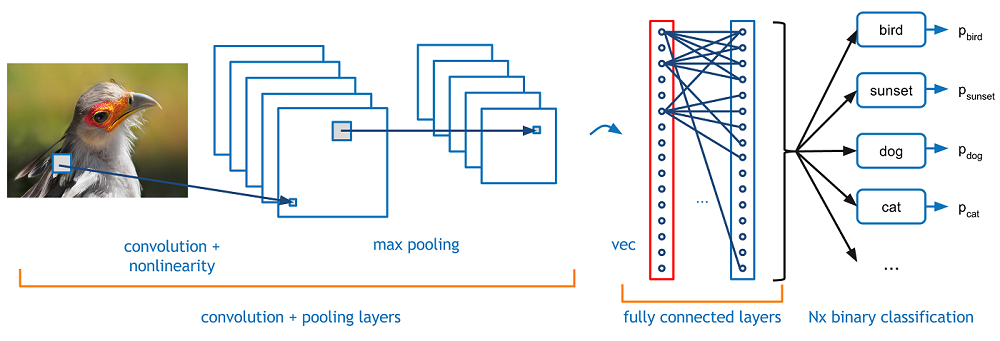
\includegraphics[width=\textwidth]{Images/4_cnn_structure.png}
	\caption{Typical CNN Structure. Convolution layers with ReLU activation (nonlinearity) are followed by pooling layers. The final layers are fully connected, using softmax activation to generate a probability distribution.}
	\small Image taken from \cite{ADeshpande2016}
	\label{convnets-structurefig}
\end{figure}

CNNs typically consist of alternating convolutional layers (see Section \ref{convnets-convlayer}) and max pooling layers (see Section \ref{convnets-pool}), as shown in Figure \ref{convnets-structurefig}. The convolutional layers identify significant visual features, however they introduce a large number of variables into the network. Max pooling layers occur after convolutional layers to reduce network dimensionality. For classification tasks, the last layers of the network are fully connected to ensure the final outputs match the structure of the given responses. Softmax activation (see Section \ref{nnets-act}) is used for the final output layer to generate a probability distribution of the classifications.

\section{Convolutional layers}\label{convnets-convlayer}

The neurons of convolutional layers have a similar overall structure to that of regular neurons (see Section \ref{nnets-structure}). The input variables $X$ are multiplied with weights $W$, summed and added to a bias variable $b$. The resulting linear combination is passed through an activation function $\sigma(\cdot)$ to give the output of the neuron with activation value $a$.

The major difference between convolutional layers and regular neural network layers is the structure of the inputs and weights. Image data is two-dimensional and generally has multiple colour \textit{channels}. For example, a coloured image contains three channels: red, green, and blue. The intensity of each pixel in each channel is represented as a number such that the image forms a three-dimensional array. The weights of convolutional layers are formatted as three-dimensional arrays to accommodate for the number of colour channels. These weight arrays are element-wise multiplied with a subset of the whole image. Unlike fully connected layers, convolutional layers do not apply weights to all of the input variables at once. Instead, the weights have an array height and width much smaller than that of the input image, designed to identify particular visual features in smaller subimages. A single matrix of weights that describes a feature is called a \textit{filter}. Each convolutional layer can have multiple filters, analogous to having multiple neurons in a fully connected layer.

Each filter processes the whole image by multiplying with subimages chosen sequentially. The process, known as \textit{convolution}, begins at the top-left of the image and moves towards the bottom-right. Let the $f$-th filter of the convolultional layer be $F^{(f)}$, with dimension $M\times N \times C$. Given an input image matrix $X$, number of channels $C$, and the bias of the $f$-th filter $b^{(f)}$, the value of the convolution at element $X_{j,k}$ is given by
\begin{align}
	a_{jk}^{(f)} = \sigma\left(\sum_{c=1}^C\sum_{m=0}^{M-1}\sum_{n=0}^{N-1}X_{j+m, k+n, c}F_{m,n,c}^{(f)}  + b^{(f)}\right).
\end{align}

Let us consider an example.
\begin{example}
%\begin{figure}[h]
%\centering
%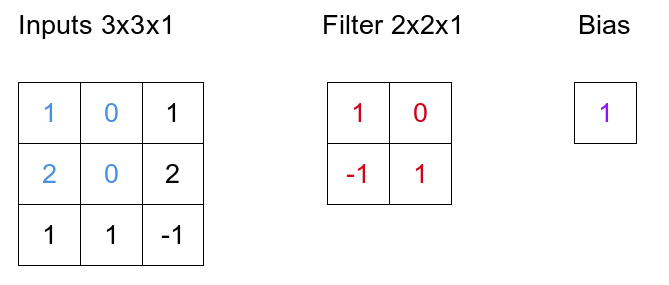
\includegraphics[scale=0.5]{Images/4_conv_eg2.png}
%\label{convnets-conv-eg}
%\end{figure}

\begin{figure}[h]
\centering
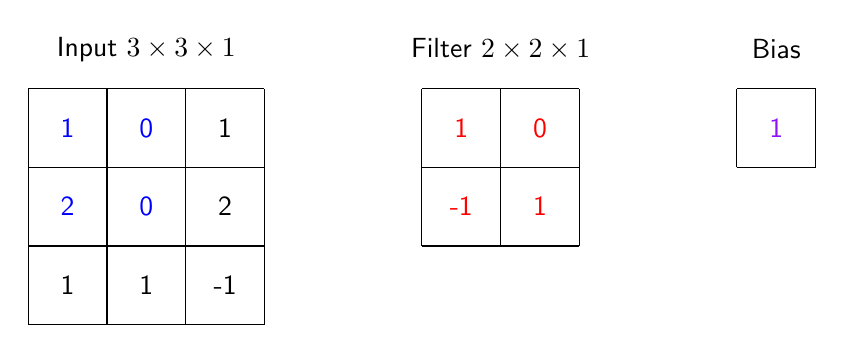
\begin{tikzpicture}[font=\sffamily]
\draw[step=1cm] (0, 0) grid (3, 3);
\draw[step=1cm] (5, 1) grid (7, 3);
\draw[step=1cm] (9, 2) grid (10, 3);

\node at (0.5, 2.5) {\color{blue}1};
\node at (1.5, 2.5) {\color{blue}0};
\node at (2.5, 2.5) {1};
\node at (0.5, 1.5) {\color{blue}2};
\node at (1.5, 1.5) {\color{blue}0};
\node at (2.5, 1.5) {2};
\node at (0.5, 0.5) {1};
\node at (1.5, 0.5) {1};
\node at (2.5, 0.5) {-1};

\node at (5.5, 2.5) {\color{red}1};
\node at (6.5, 2.5) {\color{red}0};
\node at (5.5, 1.5) {\color{red}-1};
\node at (6.5, 1.5) {\color{red}1};

\node at (9.5, 2.5) {\textcolor[rgb]{0.56,0.07,1}{1}};

\node at (1.5, 3.5) {Input $3\times3\times1$};
\node at (6, 3.5) {Filter $2\times2\times1$};
\node at (9.5, 3.5) {Bias};

\end{tikzpicture}
\end{figure}

The filter in red is multiplied element-wise with the inputs given in blue. This gives:
\begin{figure}[h]
\centering
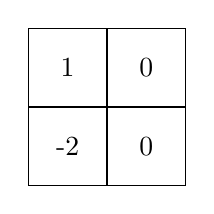
\begin{tikzpicture}
\draw[step=1cm] (0,0) grid (2, 2);
\node at (0.5,1.5) {1};
\node at (1.5,1.5) {0};
\node at (0.5,0.5) {-2};
\node at (1.5,0.5) {0};
\end{tikzpicture}
\end{figure}

Taking the sum of the products and adding the bias in purple gives the activation value $(1 + 0 + -2 + 0) + 1 = 0$. This process is iterated for all $2\times2$ subimages in the original input, giving the following output:

\begin{figure}[h]
\centering
%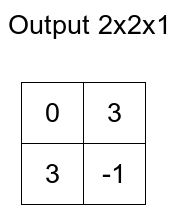
\includegraphics[scale=0.5]{Images/4_conv_eg2_2.png}
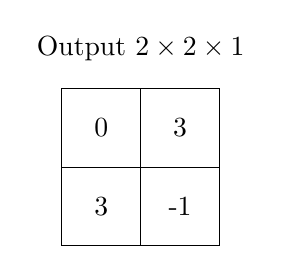
\begin{tikzpicture}

\draw[step=1cm] (0,0) grid (2, 2);
\node at (0.5,1.5) {0};
\node at (1.5,1.5) {3};
\node at (0.5,0.5) {3};
\node at (1.5,0.5) {-1};

\node at (1, 2.5) {Output $2\times2\times1$};

\end{tikzpicture}
\end{figure}

\end{example}

% Diagram of convolution algorithm
%\begin{figure}[ht]
%	\centering
%	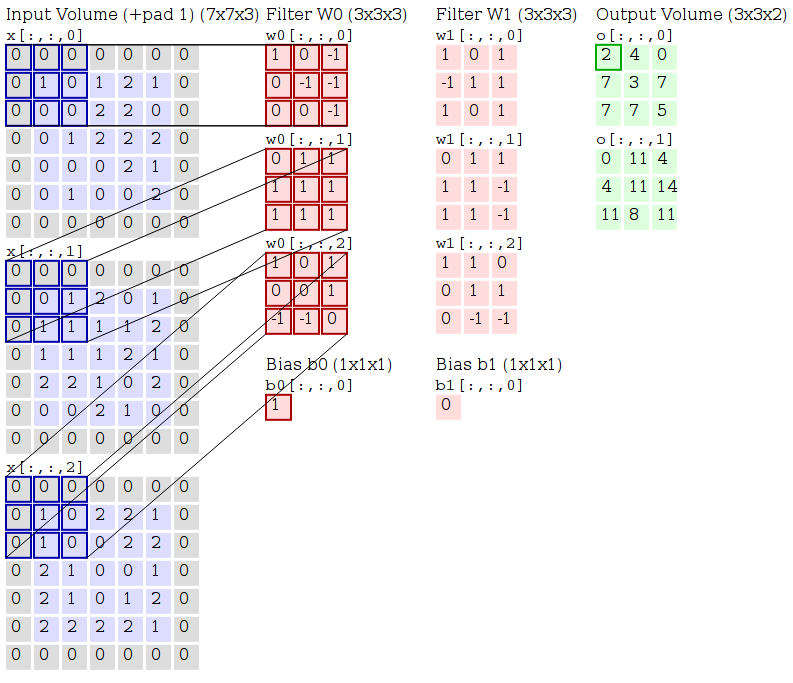
\includegraphics[scale=0.5]{Images/4_convolution.png}
%	\caption{Convolution algorithm with 2 filters of size 3x3, stride 2, zero padding 1}
%	\small Image adapted from \url{`http://cs231n.github.io/convolutional-networks/'}
%	\label{convnets-conv-alg}
%\end{figure}

%As shown in Figure \ref{convnets-conv-alg}, the convolution process starts from the top-left corner of the input volume. A subset of the image is taken at that location, with the same dimensions as the filter. The image subset and the filter are entry-wise multiplied and added together. A bias variable is added and an activation function applied as with fully connected layers. This result becomes the output of a single neuron of the convolutional layer. The filter is moved to the next location (depending on the size of the stride) to build the value of the next neuron.

The arrays output by the convolutional filters are bound together to form a three-dimensional array, with depth dependent on the number of filters in the layer.

The convolution process involves a very large number of variables, many of which are redundant when identifying important features. A number of techniques have been developed to control how the subimages are chosen, reduce image dimensionality, speed up processing, and provide flexiblity in network design. We now discuss some of these methods.

\subsection*{Zero padding}\label{convnets-pad}

During convolution, the filters are only placed within the boundaries of the input image, resulting in loss of dimension from the borders. For an input image with dimension $J \times K$ and a filter with dimension $M \times N$, the filter output will be of dimension $(J - M + 1)\times (K - N + 1)$. This places a limit on the number of convolutional layers used before the image dimension becomes too small for further convolution.

\textit{Zero padding} surrounds the edges of the input image with $P$ layers of zeros, increasing the input dimension to  $(J+2P) \times (K+2P)$. When convolution takes place, the resulting image size has dimension $(J+2P - M + 1) \times (K + 2P - N + 1)$. The value of $P$ can be set such that the convolution maintains the original image dimension, allowing the network to continue applying convolution to outputs, thus producing very deep networks \citep{GoogLeNet2015}.

\subsection*{Stride}\label{convnets-stride}

Convolving filters at all possible locations of large input images results in lengthy training time and large outputs. Applying the convolution of filters at every $S$-th subimage reduces the number of variables whilst maintaining use of the whole input image. The magnitude of the filter movement is known as the \textit{stride}.

An input image with dimension $J \times K$ convolved with a filter with dimension $M \times N$, with padding $P$ and stride $S$, will have an output dimension of $\left(\left\lfloor (J + 2P - M)/S\right\rfloor + 1\right) \times \left(\left\lfloor (K + 2P - N)/S \right\rfloor + 1\right)$.

\section{Pooling layers}\label{convnets-pool}

Convolutional layers are followed by pooling layers to reduce dimensionality whilst retaining variables that identify significant features \citep{ADeshpande2016}. The model is only interested in identifying variables for classification and does not need the location to be highly specific. A sliding window of size $M\times M$ and stride $S$ is applied to the top-left of the image input and moves across the image similarly to the convolutional layers. At each location, the pooling layer outputs a single value, which collectively form a matrix of reduced dimension to the input.

For \textit{max pooling}, the values output are the maximum values of all inputs in each sliding window. Max pooling is a preferred pooling method as it emphasises features of interest located by the previous convolutional layer.

\section{ReLU activation}\label{convnets-act}

The ReLU activation function, as defined in Section \ref{nnets-act}, is frequently used for  convolutional neural networks. Computation time can become very large as there are a large number of variables. The ReLU function can be computed very quickly and so is a common choice for convolutional neural networks \citep{ADeshpande2016}. Additionally, the ReLU activation function is also able to avoid the vanishing gradient problem (see Section \ref{nnet-vanishinggradprob}).


%Convolutional Neural Networks are very similar to traditional neural networks, but make the assumption that the input data are images.
%The neurons of a convNet are arranged in 3D. 
%http://cs231n.github.io/convolutional-networks/
%
%Input layer: raw pixel values, with width, height and color channels
%Conv layer: Compute output for regions of input. Each computes a dot product between weights and a region that they are connected to.
%ReLU: elementwise activation function.
%Pool: downsampling
%FC - fully connected: each neuron here is connected to all previous.
%
%Conv layer has a set of learnable filters. The filter might have only a small size, but will slide (convolve) across the image, computing dot products at each position.

%https://stats.stackexchange.com/questions/154879/a-list-of-cost-functions-used-in-neural-networks-alongside-applications
%https://pappubahry.com/misc/neural/nielsen_1/
% http://neuralnetworksanddeeplearning.com/

%Good animated representation: https://ujjwalkarn.me/2016/08/11/intuitive-explanation-convnets/
%
%https://medium.com/technologymadeeasy/the-best-explanation-of-convolutional-neural-networks-on-the-internet-fbb8b1ad5df8
%
%https://tensorflow.rstudio.com/tensorflow/articles/tutorial_mnist_beginners.html
%
%https://adeshpande3.github.io/A-Beginner%27s-Guide-To-Understanding-Convolutional-Neural-Networks-Part-2/
%
%https://tech.hbc.com/2016-05-18-fully-connected-to-convolutional-conversion.html


%\section{R-CNN}
%Purpose is to take in an image, and draw bounding boxes over all of the objects. Train to find 4D output (x, y, width, height) of object. Use L2 distance loss between prediction and 'ground truth'.
%
%Done by attaching a fully connected layer to the last conv layer. Separate classification layers and box coord layers. 
%Accuracy determined by Intersection over Union (ioU) area. 






%%%%%%%%%%%%%%%%%%%%%%%%%%%%%%%%%%%%%%%%%%%%%%%%%%%%%%%%%%%%%%%%%%%%%%%%%%%

%\clearpage

\addcontentsline{toc}{chapter}{References}

\bibliographystyle{apalike}
\bibliography{bibliography.bib}

%\bibliographystyle{apacite}
%\bibliography{mybib.bib}



%\documentclass[honours,12pt,twoside]{unswthesis}

\usepackage{afterpage}
\usepackage{amsfonts}
\usepackage{amsmath}
\usepackage{amssymb}
\usepackage{amsthm}
\usepackage[english]{babel}
\usepackage{graphicx}
\usepackage{natbib}
\usepackage[utf8]{inputenc}
\usepackage{latexsym}
\usepackage{url}
\usepackage{todonotes}
\usepackage{tikz}
\usepackage{pdfpages}
\usetikzlibrary{arrows}
\usepackage{float}

\usepackage{booktabs}
\renewcommand{\arraystretch}{1.2}


%%%%%%%%%%%%%%%%%%%%%%%%%%%%%%%%%%%%%%%%%%%%%%%%%%%%%%%%%%%%%%%%%
%
%  The following are some simple LaTeX macros to give some
%  commonly used letters in funny fonts. You may need more or less of
%  these
%
\newcommand{\R}{\mathbb{R}}
\newcommand{\Q}{\mathbb{Q}}
\newcommand{\C}{\mathbb{C}}
\newcommand{\N}{\mathbb{N}}
\newcommand{\F}{\mathbb{F}}
\newcommand{\PP}{\mathbb{P}}
\newcommand{\T}{\mathbb{T}}
\newcommand{\Z}{\mathbb{Z}}
\newcommand{\B}{\mathfrak{B}}
\newcommand{\BB}{\mathcal{B}}
\newcommand{\M}{\mathfrak{M}}
\newcommand{\X}{\mathfrak{X}}
\newcommand{\Y}{\mathfrak{Y}}
\newcommand{\CC}{\mathcal{C}}
\newcommand{\E}{\mathbb{E}}
\newcommand{\cP}{\mathcal{P}}
\newcommand{\cS}{\mathcal{S}}
\newcommand{\A}{\mathcal{A}}
\newcommand{\ZZ}{\mathcal{Z}}

%%%%%%%%%%%%%%%%%%%%%%%%%%%%%%%%%%%%%%%%%%%%%%%%%%%%%%%%%%%%%%%%%%%%%
%
% The following are much more esoteric commands that I have left in
% so that this file still processes. Use or delete as you see fit
%
\newcommand{\bv}[1]{\mbox{BV($#1$)}}
\newcommand{\comb}[2]{\left(\!\!\!\begin{array}{c}#1\\#2\end{array}\!\!\!\right)
}
\newcommand{\Lat}{{\rm Lat}}
\newcommand{\var}{\mathop{\rm var}}
\newcommand{\Pt}{{\mathcal P}}
\def\tr(#1){{\rm trace}(#1)}
\def\Exp(#1){{\mathbb E}(#1)}
\def\Exps(#1){{\mathbb E}\sparen(#1)}
\newcommand{\floor}[1]{\left\lfloor #1 \right\rfloor}
\newcommand{\ceil}[1]{\left\lceil #1 \right\rceil}
\newcommand{\hatt}[1]{\widehat #1}
\newcommand{\modeq}[3]{#1 \equiv #2 \,(\text{mod}\, #3)}
\newcommand{\rmod}{\,\mathrm{mod}\,}
\newcommand{\p}{\hphantom{+}}
\newcommand{\vect}[1]{\mbox{\boldmath $ #1 $}}
\newcommand{\reff}[2]{\ref{#1}.\ref{#2}}
\newcommand{\psum}[2]{\sum_{#1}^{#2}\!\!\!'\,\,}
\newcommand{\bin}[2]{\left( \begin{array}{@{}c@{}}
				#1 \\ #2
			\end{array}\right)	}
%
%  Macros - some of these are in plain TeX (gasp!)
%
\newcommand{\be}{($\beta$)}
\newcommand{\eqp}{\mathrel{{=}_p}}
\newcommand{\ltp}{\mathrel{{\prec}_p}}
\newcommand{\lep}{\mathrel{{\preceq}_p}}
\def\brack#1{\left \{ #1 \right \}}
\def\bul{$\bullet$\ }
\def\cl{{\rm cl}}
\let\del=\partial
\def\enditem{\par\smallskip\noindent}
\def\implies{\Rightarrow}
\def\inpr#1,#2{\t \hbox{\langle #1 , #2 \rangle} \t}
\def\ip<#1,#2>{\langle #1,#2 \rangle}
\def\lp{\ell^p}
\def\maxb#1{\max \brack{#1}}
\def\minb#1{\min \brack{#1}}
\def\mod#1{\left \vert #1 \right \vert}
\def\norm#1{\left \Vert #1 \right \Vert}
\def\paren(#1){\left( #1 \right)}
\def\qed{\hfill \hbox{$\Box$} \smallskip}
\def\sbrack#1{\Bigl \{ #1 \Bigr \} }
\def\ssbrack#1{ \{ #1 \} }
\def\smod#1{\Bigl \vert #1 \Bigr \vert}
\def\smmod#1{\bigl \vert #1 \bigr \vert}
\def\ssmod#1{\vert #1 \vert}
\def\sspmod#1{\vert\, #1 \, \vert}
\def\snorm#1{\Bigl \Vert #1 \Bigr \Vert}
\def\ssnorm#1{\Vert #1 \Vert}
\def\sparen(#1){\Bigl ( #1 \Bigr )}

\newcommand\blankpage{%
    \null
    \thispagestyle{empty}%
    \addtocounter{page}{-1}%
    \newpage}
    
%%%%%%%%%%%%%%%%%%%%%%%%%%%%%%%%%%%%%%%%%%%%%%%%%%%%%%%%%%%%%%
%
% These environments allow you to get nice numbered headings
%  for your Theorems, Definitions etc.  
%
%  Environments
%
%%%%%%%%%%%%%%%%%%%%%%%%%%%%%%%

\newtheorem{theorem}{Theorem}[section]
\newtheorem{lemma}[theorem]{Lemma}
\newtheorem{proposition}[theorem]{Proposition}
\newtheorem{corollary}[theorem]{Corollary}
\newtheorem{conjecture}[theorem]{Conjecture}
\newtheorem{definition}[theorem]{Definition}
\newtheorem{example}{Example}
\newtheorem{remark}[theorem]{Remark}
\newtheorem{question}[theorem]{Question}
\newtheorem{notation}[theorem]{Notation}
\numberwithin{equation}{section}

%\begin{document}

\chapter{Existing methodologies}\label{litrev}

This chapter outlines existing models in more detail, and discusses the impact of including location-based variables. In particular, we examine the variable thresholds developed by Yokoyama et al. \cite{Yokoyama2007} and the location-based \textsc{cnn} by Ghafoorian et al. \cite{GhafoorianM.2017Dml3}.

\section{Thresholding}\label{litrev-threshold}

This section describes an existing attempt to automate the identification of lacunes by developing and applying thresholds for certain variables. In 2007, Yokoyama et al. \cite{Yokoyama2007} developed an algorithm that identifies lacune candidates by examining their \textit{area}, \textit{circularity} and \textit{gravitational centre}. Area $A$ is the number of pixels that the candidate lacune covers. Circularity is given by $C = 4\pi\times\dfrac{A}{\ell^2}$, where $\ell$ is the perimeter of the candidate lacune. The gravitational centre is given by $(g_x, g_y) = \bigg(\dfrac{1}{n}\sum_{i=1}^nx_i, \dfrac{1}{n}\sum_{i=1}^ny_i\bigg)$.

Yokoyama et al. \cite{Yokoyama2007} claim that lacunes primarily occur in the basal ganglia, a structure at the centre of the brain. Thus the search for lacunes was limited to a central circular region with the coordinates of the centre and the radius specified for each scan.

Candidate lacunes satisfy thresholds based on area, circularity and gravitational centre. The thresholds are established dependent on the intensity of the surrounding structures. For this reason, candidates are separated into two categories: isolated lacunes and those surrounded by \textsc{wmh}. Isolated lacune candidates are determined by extracting the cerebral ventricle and calculating the mean pixel intensity. Candidates are determined as regions with an intensity below 70\% of the mean value. Isolated candidate lacunes satisfy the inequalities
\begin{align*}
	& 19 \le A \le 200, \\
	& 0.45 \le C,\text{ and } \\
	& (g_x - c_x)^2 + (g_y - c_y)^2 < 12000,
\end{align*}
where $(c_x, c_y)$ is the centre of the circular region of interest. The region defining accepted candidates is shown in Figure \ref{litrev-area-circ}.

% Fig. 5 from Yokoyama 2007 showing the bounds for area and circularity for false and true lacunes.
\begin{figure}[ht]
\centering
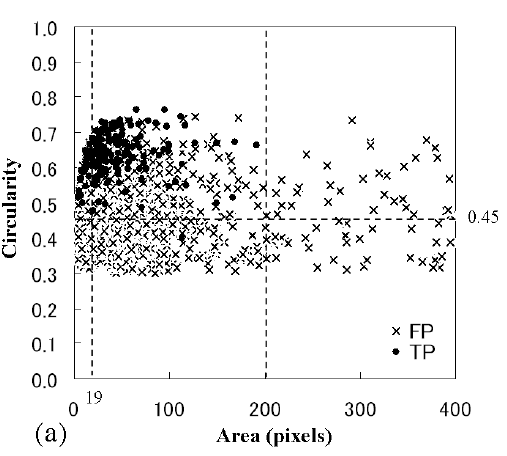
\includegraphics[scale=0.7]{Images/5_yokoyama_reg.png}
\caption{Relationship between candidate lacune area and circularity on the training data set.}
\small Image taken from \cite{Yokoyama2007}
\label{litrev-area-circ}
\end{figure}

Lacunes that appear next to \textsc{wmh} are more difficult to extract and so are treated separately. These candidates are determined by taking intensity differences between the region and the cerebral ventricle \textsc{csf}. Candidates satisfy the inequalities,
\begin{align*}
	25 \le A \le 100\text{ and } 0.48 \le C.
\end{align*}

Once candidates are identified, the model eliminates false-positives by examining the T1-weighted scans. False-positive removal is based on a candidate's location, area and gravitational centre.

The data set used to develop the model consisted of 100 scans, totalling 832 axial slices. Model training and testing consisted of 20 and 80 scans respectively. The final algorithm exhibited a \textit{sensitivity} rate (correct classification of positives) of 90.1\% and averaged 1.7 false-positives per slice.

Although the testing sensitivity was high, it was insufficient for the model to be usable on its own. Model improvement is required before it can be used to aid clinicians reliably. The low sensitivity rate may be the result of a restricted search area. Yokoyama et al. \cite{Yokoyama2007} made the assumption that lacunes only occur deep within the brain, through the basal ganglia. This was the motivation behind defining a circular search region and extracting the cerebral ventricles. However, this assumption is not always satisfied. Though less common, lacunes have been found in other brain regions, including the cerebrum (see Section \ref{data}). Restricting the search area may inadvertently exclude lacunes from detection.

The model by Yokoyama was dependent on a number of existing architectures. The first is the identification and extraction of particular brain regions. In this model, Yokoyama et al. were able to use existing binarisation techniques to extract the cerebral ventricle. Each sample also requires a calculated area, circularity and gravitational centre. Each of these calculations requires sufficient time and resources particularly if these calculations are to be conducted manually.

The comparatively low sensitivity may also be the result of too few variables. An indicator for hyperintensive rims and the area and circularity from associated \textsc{flair} images may improve the sensitivity rate. This was not tested due to time and data constraints.

%
%
%This section describes an existing attempt to automate the identification of lacunes, with false-positives reduced by accepting candidates within established thresholds for certain variables. In 2007, Yokoyama et al. \cite{Yokoyama2007} developed an algorithm that examines lacune candidate area, circularity and gravitational centre. Candidates are chosen such that they satisfy particular thresholds, where these thresholds are dependent on the candidate's location and surrounding hyperintense structures. The resulting model exhibited a \textit{sensitivity} rate (correct classification of positives) of 90.1\% and averaged 1.7 false-positives per axial slice.
%
%% Fig 1. from Yokoyama 2007 that shows structure of algorithm
%\begin{figure}[ht]
%\centering
%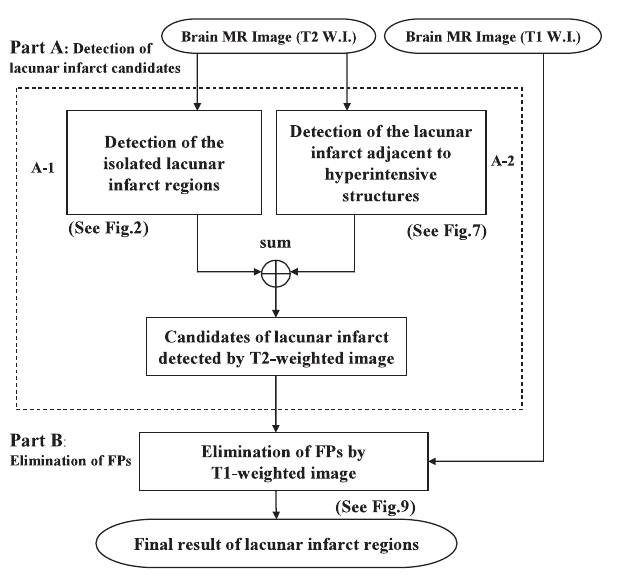
\includegraphics[scale=0.7]{Images/5_yokoyama_model.png}
%\caption{Model structure by Yokoyama et al. \citep{Yokoyama2007}}
%\label{litrev-yokoyama-structure}
%\end{figure}
%
%The algorithm is comprised of several stages, shown in Figure \ref{litrev-yokoyama-structure}. In the first phase, T2-weighted images are used to identify candidate lacunes. These candidates are one of two types: lacunes that are isolated, and those that are found next to \textsc{wmh}.
%
%% Fig. 3 from Yokoyama 2007
%\begin{figure}[ht]
%	\centering
%	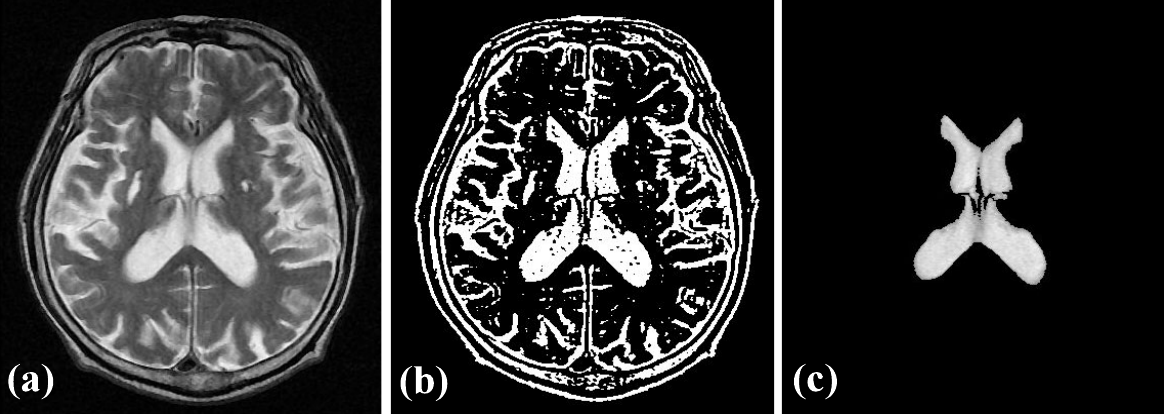
\includegraphics[width=\textwidth]{Images/5_extract_ventricle.png}
%	\caption{Extraction of the cerebral ventricle.}
%	\small Image taken from \cite{Yokoyama2007}
%	\label{litrev-yokoyama-ventricles}
%\end{figure}
%
%Isolated lacune candidates are determined by considering the mean pixel value of the cerebral ventricles. The ventricles are extracted from the image, shown in Figure \ref{litrev-yokoyama-ventricles}, and the threshold for lacune identification is set at 70\% of the mean pixel value. Yokoyama et al. \cite{Yokoyama2007} claim that lacunes primarily occur in the basal ganglia, a structure at the centre of the brain. Hence, the detection region is limited to a central circular region with determined centre and radius for each scan. 
%
%Lacunes are identified by considering three properties: area, circularity and gravitational centre. \textit{Area}, $A$, is the number of pixels that the candidate lacune covers. \textit{Circularity}, $C$, is given by $	C = 4\pi \times \dfrac{A}{\ell^2}$, where $\ell$ is the perimeter of the candidate lacune. The \textit{gravitational centre} is the central coordinate of the candidate lacune, given by $(g_x, g_y) = \bigg(\dfrac{1}{n}\sum_{i=1}^nx_i, \dfrac{1}{n}\sum_{i=1}^ny_i\bigg)$. Candidate lacunes satisfy the inequalities
%\begin{align*}
%	& 19 \le A \le 200, \\
%	& 0.45 \le C,\text{ and } \\
%	& (g_x - c_x)^2 + (g_y - c_y)^2 < 12000,
%\end{align*}
%where $(c_x, c_y)$ is the centre of the circular region of interest. The candidate regions for area and circularity are shown in Figure \ref{litrev-area-circ}.
%


%Lacunes that appear next to \textsc{wmh} are more difficult to extract and so are treated separately. Yokoyama et al. use the difference between two circular filters of radii 1 and 8 pixels. False-positives are eliminated by taking the difference in intensity between candidate lacunes and cerebral ventricle \textsc{csf}. Using the same definitions for area and circularity as with isolated lacunes, candidates next to \textsc{wmh} satisfy
%\[
%	25 \le A \le 100\text{ and } 0.48 \le C.
%\]
%Once candidates are identified, the model eliminates false-positives by examining the T1-weighted scans. False-positive removal is based on candidate location, area and gravitational centre.
%
%The algorithm was trained on 100 scans, containing 832 slices in total. 20 of these scans were used for training and 80 for testing.
%
%The second phase of training reduced the number of false-positives by 68\%. However, of the four types of false-positives, enlarged perivascular spaces had no reduction, as shown in Figure \ref{litrev-yokoyama-fps}. Other false-positives types include those at the edge of the cerebral parenchyma (\textsc{ecp}), periventricular high-signal regions (\textsc{pvh}), and those around the cerebral ventricle (\textsc{cv}), and will not be discussed. This model is instead more likely to differentiate lacunes from the edge of the cerebrum, hyperintensities and the cerebral ventricle.
%
%% Table 1 from Yokoyama 2007. Elimination of false-positives - all PVS got through!
%\begin{figure}[ht]
%	\centering
%	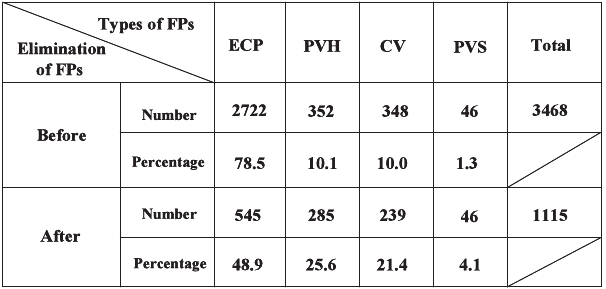
\includegraphics[width=0.8\textwidth]{Images/5_yokoyama2007testing.png}
%	\caption{Elimination of false-positives. Perivascular spaces (\textsc{pvs}) see no reduction. They make only 4.1\% of false-positives under the definition in \cite{Yokoyama2007}.}
%	\small Image taken from \cite{Yokoyama2007}
%	\label{litrev-yokoyama-fps}
%\end{figure}
%
%Yokoyama et al. suggest that further reductions in false-positives could be attained through the use of FLAIR imaging. Lacunes are found to have a low intensity in T1-weighted imaging and a high intensity in T2-weighted imaging. In FLAIR imaging, lacunes are also found to have a low intensity, but not as low as the surrounding CSF, and often have a hyperintense rim \cite{WardlawJ.M.2013Nsfr}. 
%
%Further improvements could be made by using multiple slices for each candidate, increasing image context. Using 3D information, the axial slices above and below a candidate could be used to further eliminate false-positives. This is particularly relevant when a candidate lacune appears on only a single axial slice, or when the candidate diverges from the indicative ovoid shape in surrounding slices. Including this information would assist in differentiation between lacunes and perivascular spaces, since perivascular spaces can appear rectangular along the coronial or saggital plane.
%
%\subsection*{Concerns}
%
%Although the testing sensitivity was high, it was not high enough for the model to be usable on its own. Model improvement is required before it can be used to aid clinicians reliably.
%
%Yokoyama et al. made the assumption that lacunes only occur deep within the brain, within and surrounding the basal ganglia. This was the motivation behind extracting data around the cerebral ventricle. However, this assumption is not always satisfied. Though less common, lacunes have been found in other brain regions, including the cerebrum.
%
%The feature definitions used for the model also make it difficult to identify perivascular spaces. In this model, perivascular spaces were defined as small, circular regions of diameter less than 3 mm, located at the lower basal ganglia. This specification meant that the model was not sensitive to enlarged perivascular spaces, which can have a diameter up to 10 mm and can occur anywhere in the grey and white matter of the brain \cite{WardlawJ.M.2013Nsfr}. This change in definition contributes to the seemingly low false-positive presence that PVS exhibit in the data.
%
%It should be mentioned that this model is dependent on a number of existing architectures. The first is the identification and extraction of particular brain regions. In this model, Yokoyama et al. were able to use existing binarisation techniques to extract the cerebral ventricle. Each sample also requires a calculated area, circularity and gravitational centre. Each of these calculations requires sufficient time and resources, particularly if these calculations are to be conducted manually.
%
%Finally, the proportion of false-positives is still relatively high. The sensitivity after the second phase is 90\%, which is substantial but still not accurate enough to warrant full automation of the process. Of particular concern is the proportion of perivascular spaces falsely marked as lacunes. Though they appear similar to lacunes, perivascular spaces do present some slight shape and intensity differences.

%In 2012, Wang et al. \cite{WangY.2012Msow} developed an algorithm that labels three features: \textsc{wmh}, lacunes in the cerebral cortex (cortical infarcts), and lacunes beneath the cerebral cortex (lacunar infarcts). The model was provided with 272 scans, each capturing T1-weighted, T2-weighted and \textsc{flair} images. In the first stage of the algorithm, the T1-weighted images are used to segment the brain into white matter, grey matter and \textsc{csf}. Average intensities are calculated for each segmented region and for each image type. Candidate features are identified based on their intensity relative to these these averages. The resulting sensitivity rate for lacunes is 80.6\% and 006 false-positives per slice.

\section{Machine learning}\label{litrev-ml}

This section describes a number of models that were developed using machine learning techniques. The model by Yokoyama et al. \cite{Yokoyama2007} suffered from a lower sensitivity rate, possibly caused by lack of information extracted from the images. Machine learning techniques seek to identify features that are not always easily interpreted, but have had promising results. 

The first attempts were made by Uchiyama et al. in 2007 \cite{Uchiyama20071554, Uchiyama2007b} as a continuation of the model by Yokoyama et al. \cite{Yokoyama2007}. The data consisted of 132 scans totalling 1143 images of T1 and T2 weighting. Once candidates have been identified, the models undergo false-positive reduction. Twelve location based features are identified: x and y coordinates, intensity differences in T1 and T2, four nodule shape variables, and four combined nodule and linear shape variables.

These features were input into two different machine learning algorithms: a support vector machine (machine learning algorithm for discrimination tasks) and a neural network. The support vector machine resulted in a sensitivity of 96.8\%, with 0.76 false-positives per slice. The second model was a neural network, with a sensitivity of 96.8\% and 0.30 false-positives per slice.

In 2015, Uchiyama et al. \cite{Uchiyama2015} augmented their previous models by matching candidates with a number of lacune templates. To improve the efficiency of the matching process, data was reduced to a lower dimensional space through principal component analysis. False-positives were reduced by 34.1\%, with the final model having a sensitivity of 96.8\% and 0.47 false-positives per slice.

The substantial rise in sensitivity in comparison to the original model \cite{Yokoyama2007} confirms that additional information was required to improve lacune detection. However the included variables remain location dependent and require either existing algorithms or significant time resources during data collection.


%\section{Yokoyama 2007}
%
%Lacunar infarct regions are classified into two types: isolated regions and regions next to hyperintensities. Isolated lacune candidates are found using multiple-phase binarisation. Candidates next to hyperintense structures are detected by pre-processing and subtracting images. Candidate regions are generated based on area, circularity and gravitational centre. False-positives are first reduced by removing candidates at the edge of the image. Next compare the candidates against mean pixel values of surrounding circular regions.
%20 lacune samples were used to adjust area, circularity and gravitational centre thresholds. 673 images used for testing. Sensitivity 90.1\%, specificity 30.0\%, 1.7 false-positives per slice.
%
%\section{Uchiyama 2007a}
%
%Data consists of 1143 of T1 and T2 weighted images each, from 132 scans. The search region was restricted (to what?). Initial candidates found by using top-hat transforms and multiple-phase binarisation to T2 weighted images. False-positives eliminated by determining 12 features: x and y coordinates, intensity differences in T1 and T2, and by extracting 4 scales of nodular component images, and 4 scales of nodular and linear component images.
%
%In this first model type, the 12 features were processed through a support vector machine. This resulted in a sensitivity of 96.8\%, with 0.76 false-positives per slice.
%
%\section{Uchiyama 2007b}
%
%This model was identical to the first (Uchiyama 2007a), with the difference that the 12 features were passed through a neural network instead of a support vector machine. This resulted in a sensitivity of 96.8\%, with 0.30 false-positives per slice.
%
%\section{Uchiyama 2008}
%
%Developed CAD scheme for classification of lacunes and perivascular spaces. 109 MRI scans of T1 and T2-weighted images. 89 lacune images and 20 enlarged perivascular spaces. White top-hat transform to enhance T2 images. Grey-level thresholding to segment lesions. Determine the size, shape, location, and T1 and T2 intensities. These features were input into a neural network to distinguish between lacunes and perivascular spaces. Area under ROC curve (true positive/false-positive ratio - only good for discriminant analysis) of 0.945.
%
%\section{Uchiyama 2015}
%
%Improvement on their previous model (96.8\% sensitivity and 0.71 false-positives per slice), by template matching in the eigenspace. However, large number of templates needed, and cross-correlation is time consuming. To resolve these issues, template matching was used in a lower dimensional space via principal component analysis. Dataset consisted of 1143 images of T1 and T2, from 132 patients (same dataset as 2007 studies?). 34.1\% of false-positives eliminated from previous attempt. Final performance was 96.8\% sensitivity, 0.47 false-positives per slice.
%
%\section{Wang 2012}
%
%Wang et al. label all three: \textsc{wmh}, cortical infarcts and lacunar infarcts. They first segment the brain tissues into white matter, grey matter and CSF using the T1-weighted scans. Hyperintense structures identified using FLAIR images. The three features are labelled based on all three weighted images, T1, T2 and FLAIR. 


%Wang et al. (2012) detect lacunes by dilating the white matter mask and using a rule-based pruning of false-positives considering their intensity levels compared to the surrounding white matter tissue.
%

%\section{Uchiyama2007a - support vector machines}

%In 2007, Uchiyama et al. \cite{Uchiyama20071554} used a machine learning algorithm to develop a computer-assisted diagnosis (CAD) program for lacune identification. In particular, false-positive reduction took the form of a support vector machine (SVM).
%
%Their data consisted of 132 MRI scans, each with T1-weighted and T2-weighted images, giving a total of 1143 axial slices in the dataset. 
%
%Similar to the method conducted by Yokoyama et al. \cite{Yokoyama2007}, Uchiyama et al. identified candidate lacunes of two forms: isolated lacunes, and those close to the cerebral ventricle. Isolated lacunes were determined by establishing a threshold, as these points exhibit a higher intensity compared to the surrounding tissue. For lacunes close to the cerebral ventricle, their higher intensity can be masked by the intensity of the surrounding ventricle. To address this, Uchiyama et al. used top-hat transforms on the T2-weighted images, a method that is specialised for extracting small details from image data.
%
%% Candidate lacune identification
%\begin{figure}[ht]
%	\centering
%	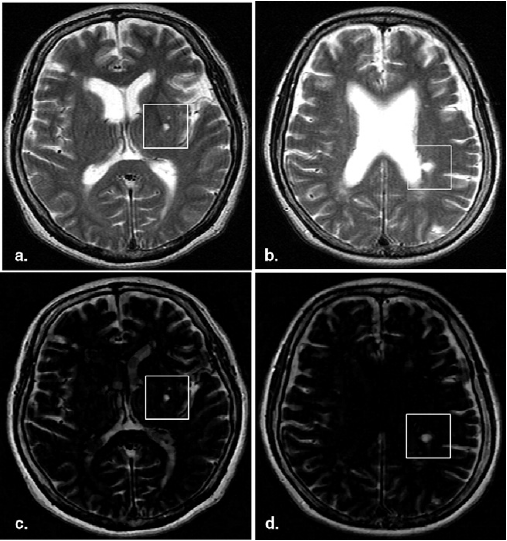
\includegraphics[width=0.8\textwidth]{Images/5_uchiyama_candidates.png}
%	\caption{Candidate lacune detection. Isolated lacune in a), with resulting top-hat transform shown in c). Lacune in b) is next to the cerebral ventricle, with top-hat transform shown in d).}
%	\small Image taken from \cite{Uchiyama20071554}
%\end{figure}
%
%false-positives were reduced using support vector machines. 12 features were used in false-positive reduction, including the candidate's x and y location, signal differences in the T1-weighted and T2-weighted images, and filtered images based on 4 nodular components and 4 combined nodular and linear components. This model produced a sensitivity of 96.8\%, with 0.76 false-positives per slice.
%
%\subsection*{Concerns}
%
%Model sensitivity is high enough to warrant usage of the model, though not high enough for full dependency. As described by Uchiyama et al., the model was designed as a CAD scheme, to run alongside manual rating by clinicians. The model still requires a user to oversee and confirm its results. 
% 
%Similar to the model developed by Yokoyama et al. \cite{Yokoyama2007}, the model developed by Uchiyama et al. was not able to distinguish between lacunes and enlarged perivascular spaces. Despite the data containing analysis on the nodular and linear nature of the candidate, the model was unable to make this distinction. Therefore, users of the CAD system must take care to confirm that the suggested candidates are not enlarged perivascular spaces.
%
%Many of the variables included in the method are dependent on other existing techniques. For instance, Uchiyama et al. explain that the nodular and linear components were determined via a newly explored filter bank technique. This technique was not well described, and as such, the model may be difficult to recreate.
%
%Another issue is the coordinate system. The model uses the x and y coordinates of the candidate to reduce false-positives. The coordinates themselves do not have any innate information about the structure of the brain. It is possible for the same x and y values to link to differing regions across brain scans. It is not certain that particular coordinates will align with a brain structure that has a significant influence on the presence of lacunes. This is especially the case for candidates deep in the brain, as many brain structures sit close together. 
%
%Under the assumption that the x and y coordinates are indicative of lacune probability, the usage of location data may still incorrectly influence outcomes. Lacunes can be found throughout the brain, including in the cerebrum. 
%
%\section{Neural Networks}
%
%Uchiyama et al. \cite{Uchiyama2007b} improve their previous model \cite{Uchiyama20071554} by altering the method used for reducing false-positives. The support vector machine was swapped with a neural network, using the same 12 input features.
%
%The sensitivity of the model to lacunar infarcts remains the same, at 96.8\%. The number of false-positives drops to 0.30 false-positives per slice.


\section{Convolutional neural networks}\label{litrev-cnn}

We will now discuss the convolutional neural network structure utilised by Ghafoorian et al. \cite{GhafoorianM.2017Dml3}. This model forms the basis of our adjusted location-independent model. This model consists of two phases; candidate generation using a \textsc{cnn}, and false-positive reduction using a 3D \textsc{cnn} and candidate location data.

\subsection*{Candidate Detection}

The data set consists of 1075 \textsc{mri} scans split into training, validation and testing sets of size 868, 96 and 111 respectively. Each scan contains two image weightings: T1-weighted and \textsc{flair}. Data samples are generated by randomly sampling axial slices of dimension 51$\times$51 pixels, each called a \textit{patch}. The model is trained to detect lacunes at the centre of each patch, returning either a positive response $(1, 0)^\intercal$ or negative response $(0, 1)^\intercal$. Combining the T1-weighted image, \textsc{flair} and response gives samples containing two 51$\times$51 pixel images and a response vector in $\mathbb{R}^2$. For use in convolution, the T1-weighted image and the \textsc{flair} image are treated as separate colour channels. Samples were generated such that there were twice as many negative samples as positive, totalling $3.2\times10^5$ training samples.

% Candidate model structure
\begin{figure}[ht]
	\centering
	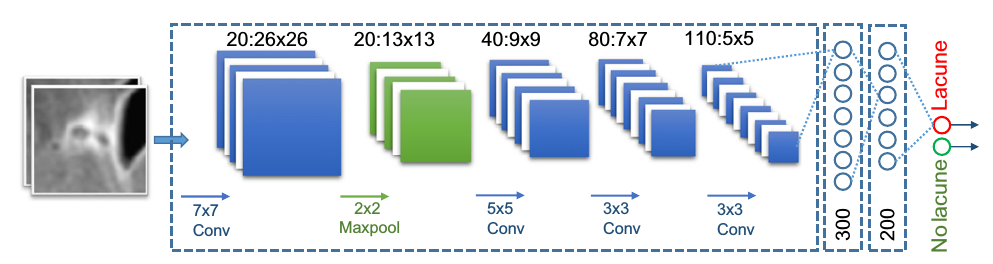
\includegraphics[width=\textwidth]{Images/5_ghafoorian_model1.png}
	\caption{Candidate detection model structure.}
	\small Image taken from \cite{GhafoorianM.2017Dml3}
	\label{litrev-ghafoorian_model1fig}
\end{figure}

The \textsc{cnn} is made of seven layers, as shown in Figure \ref{litrev-ghafoorian_model1fig}. The first four are convolutional layers, followed by three fully connected layers. The four convolutional layers contain 20, 40, 80 and 110 filters, with filter sizes 7$\times$7, 5$\times$5, 3$\times$3 and 3$\times$3 respectively. A max pooling layer is included between the first and second convolutional layer, with a filter size of 2$\times$2 and stride of 2. No zero padding is applied to the convolution or pooling layers. The convolution is followed by three fully connected layers of 300, 200 and 2 neurons.

Batch normalisation and ReLU activation is applied to all neurons. Dropout is applied to the fully connected layers, with a rate of 0.3. All weights are intialised using the He method \cite{HeKaiming2015DDiR}. Training is conducted by stochastic gradient descent with the Adam optimiser. Each training batch has a sample size of 128. A decaying learning rate is used, from $5\times10^{-4}$ to $10^{-6}$ by the last epoch.

Cross-entropy loss is used to assess the model at the end of each batch. L2-regularisation is used, with the penalty term set to $10^{-4}$. The final layer applies softmax activation to ensure the output follows a probability distribution. An early stopping algorithm is used such that the model with the highest validation accuracy is saved.

Ghafoorian et al. comment that the model can be computationally intensive to run on many data points. To improve speed, the fully connected layers are converted into convolutional layers.

Candidate lacunes are identified by feeding 51$\times$51 samples of the tested scan through the trained \textsc{cnn}. For each given sample, the model outputs a lacune classification probability. Once this has been completed for the whole volume, a 10$\times$10 sliding window identifies local maximums in the resulting probabilities. Sliding window samples with lacune probabilities below 0.1 are removed and the remaining samples are lacune candidates to be input into the second phase of the model. Note that there were no performance diagnostics provided for the first model stage.

%
%Entire model is made up of two neural networks.
%
%The first is trained such that it detects candidate lacunes.
%
%The second then takes the candidate lacunes, and processes them through a more thorough 3D CNN to finalise the outcome.
%
%\subsection{First Phase - Candidate Detection}
%
%Takes in 51x51 samples, where the T1 and FLAIR components are treated as separate channels. Twice as many negative samples as positive, with a total of 320K for training.
%
%Seven layer CNN:
%- 4 convolutional, with 20, 40, 80, 110 filters, with size 7x7, 5x5, 3x3, 3x3 respectively.
%- 1 pooling layer: size 2x2, stride 2, after first conv layer
%- 3 fully connected layers: sizes 300, 200 and 2
%- Softmax output layer
%
%All neurons went under batch normalisation.
%
%Weights initialised by the He method.
%
%ReLU activation to prevent vanishing gradient problem
%
%Dropout of 0.3 on fully connected layers
%
%Training conducted by stochastic gradient descent, Adam optimiser. Learning rate decayed, from 5e-4 to 1e-6
%
%Batch size of 128
%
%Categorical cross-entropy loss, with L2-regularisation (Ridge regression), lambda2 = 0.0001
%
%Early stopping - model with highest accuracy on validation set
%
%
%This method can be slow on its own. Translate the fully connected layers to convolutional layers, via shift-and-stitch method.
%
%Local maxima extraction (10x10 window) - picking those with likelihood lower than 0.1.
%
%
%Didn't mention: number of epochs to train. How pooling and convolutions were padded. Diagram implied no padding, but diagram dimensions weren't correct. 

\subsection*{False-positive reduction}

The second phase of the model serves to reduce the number of false-positives returned by the first stage of the model. This model uses a 3D \textsc{cnn}, adding additional contextual information to the image. Each data point is captured at three different resolutions, 32$\times$32$\times$5, 64$\times$64$\times$5 and 128$\times$128$\times$5, to capture varying levels of contextual information. These samples are reduced to dimension 32$\times$32$\times$5 before input into the model to lower the number of variables. In total, there were $3.85\times10^5$ samples for training, and $3.5\times10^4$ for validation. 

Each resolution is fed through its own 3D \textsc{cnn}, as shown in Figure \ref{litrev-ghafoorian_model2fig}. Each \textsc{cnn} branch contains six convolutional layers and a fully connected layer. The convolutional layers have 64, 64, 128, 128, 256 and 256 filters of sizes 3$\times$3$\times$2, 3$\times$3$\times$2, 3$\times$3$\times$1, 3$\times$3$\times$1, 3$\times$3$\times$1 and 3$\times$3$\times$1 respectively.

% False-positive reduction model structure
\begin{figure}[ht]
	\centering
	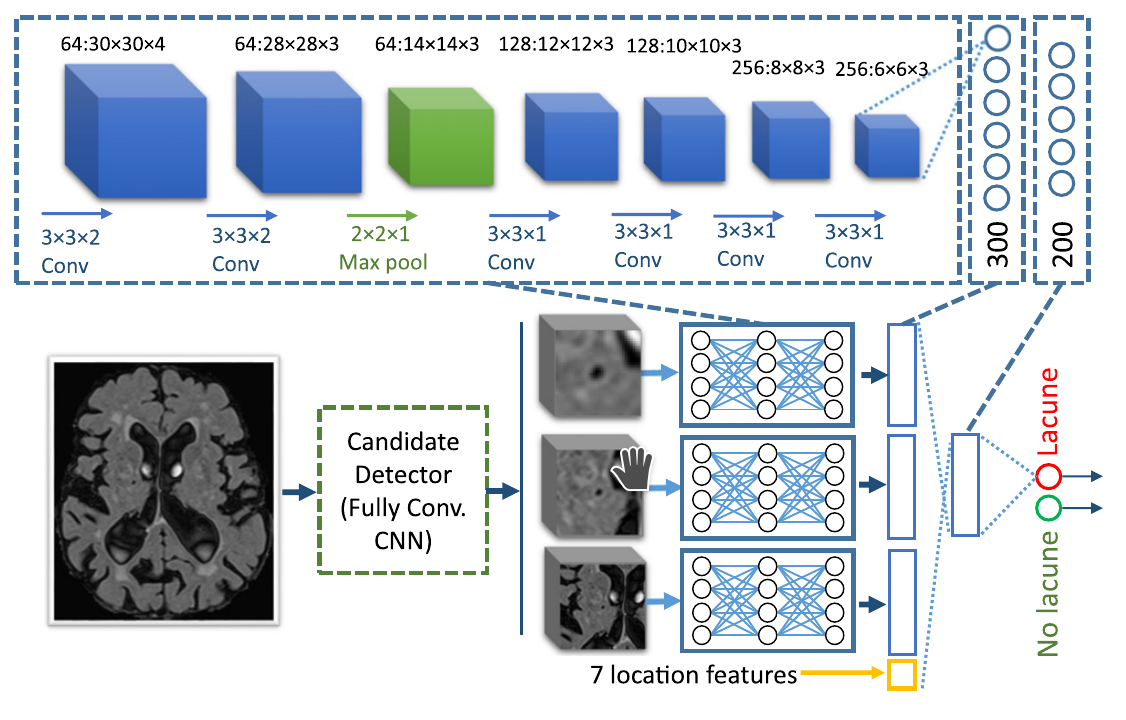
\includegraphics[width=\textwidth]{Images/5_ghafoorian_model2.png}
	\caption{False-positive reduction model structure.}
	\small Image taken from \cite{GhafoorianM.2017Dml3}
	\label{litrev-ghafoorian_model2fig}
\end{figure}

A single max pooling layer is placed after the second convolution layer, of size $2\times2\times1$. In each resolution branch, the final convolution layer is followed by a fully connected layer of 300 neurons. The $3\times300$ fully connected neurons are concatenated together with seven additional location variables. For each candidate, these location features include the $x$,$y$ and $z$ coordinates, and distances to the left and right ventricles, cortex, and midsagittal brain surface.

The 907 fully connected neurons are passed to two final fully connected layers of size 200 and 2 neurons. The final layer consists of a softmax activation to output the lacune probabilities. All weights are He initialised. All neurons, excepting the output layer, have ReLU activation and are batch normalised. The fully connected layers have a dropout rate of 0.5. 

The cost function chosen was cross-entropy with L2-regularisation and penalty parameter $2\times10^{-15}$. This was minimised using stochastic gradient descent with an Adam optimiser. The learning rate is initialised as $5\times10^{-4}$. If training accuracy drops, the learning rate decays by a factor of 2. Each training batch contained 128 samples.

The model was trained for 40 epochs, with the final model chosen to maximise validation accuracy. A number of hyper-parameters were chosen by maximising validation accuracy. These included network depth, batch size, the initial learning rate and decay factor, penalty parameter, and dropout rate. The resulting model exhibited a sensitivity of 97.4\% and an average of 0.13 false-positives per slice.




%
%\subsection{Second Phase - false-positive Reduction}
%
%This model uses data at different scales around each candidate lacune. 
%
%Input data of each point at three different scales: 32x32x5, 64x64x5, 128x128x5.
%
%Each of these scales is reduced to 32x32x5, then put through a separate branch of the network.
%
%385K training, 35K validation.
%
%Three separate branches of convNets, one for each scale. Each branch contains:
% - 6 conv layers (64, 64, 128, 128, 256,256 filters, with sizes 3x3x2, 3x3x2, 3x3x1, 3x3x1, 3x3x1, 3x3x1)
% - 1 pooling, size 2x2x1, placed after second conv layer
% - Fully connected layer of 300 neurons
% 
% The 3x300 fully connected neurons were concatenated with 7 addition location feature inputs.
% 
% These location features include:
%  - x,y,z coordinates
%  - distances from left ventricle, right ventricle, cortex and midsaggital brain surface.
%
%Then the 907 neurons are fully connected to two more fully connected layers, of size 200 and 2 neurons. 
%These are fed through a softmax classifier to output the final result.
%
%All weights are He initialised 
%
%All activations are ReLU, and are batch normalised.
%
%Fully connected layers have a dropout of 0.5.
%
%Cost function is cross entropy with L2 regularisation, lambda2 = 2e-5. 
%
%Stochastic gradient descent, Adam optimiser. Decaying learning rate, from 5e-4, decay factor of 2 when training accuracy dropped. 
%
%Training for 40 epochs, batch size of 128.
%
%Chose model with highest validation accuracy. 
%
%Hyper-parameters were also chosen such as to attain highest validation accuracy. These hyper-parameters included network depth, batch size, initial learning rate, learning decay factor, lambda2 and dropout rate. This is done during the validation stage. Make several models, with differing hyper-parameters, with performance compared using the validation set. Then whichever model performs best on this validation set is chosen, and final performance judged by the test set.
%
%Data was augmented during test time: cropping and flipping. Predictions of the 242 variants per sample were averaged.
%
%Didn't mention: stride of pooling. Assumed 2 from diagram.
% 
%\subsection{Model performance}

\section{Proposed changes}\label{litrev-changes}

The models trained by Uchiyama et. al. \cite{UchiyamaYoshikazu2007Ioad}, Yokoyama et. al. \cite{Yokoyama2007} and Ghafoorian et al. \cite{GhafoorianM.2017Dml3} rely on location variables generated for each candidate lacune. Ghafoorian et al. claimed that the inclusion of location variables helps to differentiate lacunes from perivascular spaces, which occur primarily in the basal ganglia. However, lacunes can occur throughout the brain white and grey matter \cite{WardlawJm2013Mosc} and so adding these location variables could result in incorrect classification should lacunes occur in less frequently observed regions.

The inclusion of location data requires extra data pre-processing. These variables are calculated in relation to other located brain structures, however these locations are not inherently included within \textsc{mri} scan data. Instead these variables are generated prior to model usage and require either visual estimation or a feature extraction algorithm \cite{Uchiyama2007b, UchiyamaYoshikazu2007Ioad}. If the variables are to be determined visually, the variables for each candidate lacune have to be determined separately and this would require significant extra data preparation time. If location variable extraction algorithms exist, as in the model by Uchiyama et al. \cite{UchiyamaYoshikazu2007Ioad}, additional measurement errors could also make location-based inference inaccurate.

In this study, we attempt to simplify and adapt the model by Ghafoorian et al. \cite{GhafoorianM.2017Dml3} to the available data set (see Section \ref{data}). A key component of the existing model is the removal of false-positives by analysing the three-dimensional context and location-based variables. These variables include the $x$, $y$ and $z$ coordinates, and distances between the candidate and the ventricles, cortex and midsagittal plane. Without the architecture to determine these distances, these variables have to be determined manually. In addition, the  $x$, $y$ and $z$ coordinates are not standardised between scans. Consequently, the coordinates across images do not necessarily align with the same brain structures.

The available image pre-processing pipeline (see Section \ref{data}) allows for the automated extraction of brain tissue. This may reduce the complexity of the task such that location-based variables may not be required. We therefore simplify and assess the existing model when performed on brain tissue extracted data, independent of location-based variables.


%- All previous models have made some use of location data. In particular, Ghafoorian used x/y/z, and distances from the candidate to particular brain structures. However, lacunes can appear in other regions of the brain, including regions far from the basal ganglia. The location data requires the location of the ventricles, cortex and midsaggital plane. To do this in an automated fashion requires an algorithm that can find these brain features. This requires additional estimation. Try to develop an algorithm that is independent of location data. Rely more on the image.
%
%- Instead of trimming candidates in a second phase, try to determine strong candidates from just the first phase to create an accurate CAD program. Then clinicians can be presented with candidate lacunes, and still conduct false-positive reduction themselves
%


%
%\section{Convolutional Neural Networks}
% 
%Ghafoorian et al. \cite{GhafoorianM.2017Dml3} utilised the fully convolutional nature of the initial detection model. This allows for fast image processing in comparison to fully connected layers, for 3D volumes. In addition, Ghafoorian et al. additionally utilised a multi-resolution convolutional neural network, along with 7 additional location features for false-positive reduction.
%
%\section{xgboost}
%

 


%%%%%%%%%%%%%%%%%%%%%%%%%%%%%%%%%%%%%%%%%%%%%%%%%%%%%%%%%%%%%%%%%%%%%%%%%%

%\clearpage

\addcontentsline{toc}{chapter}{References}

\bibliographystyle{apalike}
\bibliography{bibliography.bib}

%\bibliographystyle{apacite}
%\bibliography{mybib.bib}



%\documentclass[honours,12pt,twoside]{unswthesis}

\usepackage{afterpage}
\usepackage{amsfonts}
\usepackage{amsmath}
\usepackage{amssymb}
\usepackage{amsthm}
\usepackage[english]{babel}
\usepackage{graphicx}
\usepackage{natbib}
\usepackage[utf8]{inputenc}
\usepackage{latexsym}
\usepackage{url}
\usepackage{todonotes}
\usepackage{tikz}
\usepackage{pdfpages}
\usetikzlibrary{arrows}
\usepackage{float}

\usepackage{booktabs}
\renewcommand{\arraystretch}{1.2}


%%%%%%%%%%%%%%%%%%%%%%%%%%%%%%%%%%%%%%%%%%%%%%%%%%%%%%%%%%%%%%%%%
%
%  The following are some simple LaTeX macros to give some
%  commonly used letters in funny fonts. You may need more or less of
%  these
%
\newcommand{\R}{\mathbb{R}}
\newcommand{\Q}{\mathbb{Q}}
\newcommand{\C}{\mathbb{C}}
\newcommand{\N}{\mathbb{N}}
\newcommand{\F}{\mathbb{F}}
\newcommand{\PP}{\mathbb{P}}
\newcommand{\T}{\mathbb{T}}
\newcommand{\Z}{\mathbb{Z}}
\newcommand{\B}{\mathfrak{B}}
\newcommand{\BB}{\mathcal{B}}
\newcommand{\M}{\mathfrak{M}}
\newcommand{\X}{\mathfrak{X}}
\newcommand{\Y}{\mathfrak{Y}}
\newcommand{\CC}{\mathcal{C}}
\newcommand{\E}{\mathbb{E}}
\newcommand{\cP}{\mathcal{P}}
\newcommand{\cS}{\mathcal{S}}
\newcommand{\A}{\mathcal{A}}
\newcommand{\ZZ}{\mathcal{Z}}

%%%%%%%%%%%%%%%%%%%%%%%%%%%%%%%%%%%%%%%%%%%%%%%%%%%%%%%%%%%%%%%%%%%%%
%
% The following are much more esoteric commands that I have left in
% so that this file still processes. Use or delete as you see fit
%
\newcommand{\bv}[1]{\mbox{BV($#1$)}}
\newcommand{\comb}[2]{\left(\!\!\!\begin{array}{c}#1\\#2\end{array}\!\!\!\right)
}
\newcommand{\Lat}{{\rm Lat}}
\newcommand{\var}{\mathop{\rm var}}
\newcommand{\Pt}{{\mathcal P}}
\def\tr(#1){{\rm trace}(#1)}
\def\Exp(#1){{\mathbb E}(#1)}
\def\Exps(#1){{\mathbb E}\sparen(#1)}
\newcommand{\floor}[1]{\left\lfloor #1 \right\rfloor}
\newcommand{\ceil}[1]{\left\lceil #1 \right\rceil}
\newcommand{\hatt}[1]{\widehat #1}
\newcommand{\modeq}[3]{#1 \equiv #2 \,(\text{mod}\, #3)}
\newcommand{\rmod}{\,\mathrm{mod}\,}
\newcommand{\p}{\hphantom{+}}
\newcommand{\vect}[1]{\mbox{\boldmath $ #1 $}}
\newcommand{\reff}[2]{\ref{#1}.\ref{#2}}
\newcommand{\psum}[2]{\sum_{#1}^{#2}\!\!\!'\,\,}
\newcommand{\bin}[2]{\left( \begin{array}{@{}c@{}}
				#1 \\ #2
			\end{array}\right)	}
%
%  Macros - some of these are in plain TeX (gasp!)
%
\newcommand{\be}{($\beta$)}
\newcommand{\eqp}{\mathrel{{=}_p}}
\newcommand{\ltp}{\mathrel{{\prec}_p}}
\newcommand{\lep}{\mathrel{{\preceq}_p}}
\def\brack#1{\left \{ #1 \right \}}
\def\bul{$\bullet$\ }
\def\cl{{\rm cl}}
\let\del=\partial
\def\enditem{\par\smallskip\noindent}
\def\implies{\Rightarrow}
\def\inpr#1,#2{\t \hbox{\langle #1 , #2 \rangle} \t}
\def\ip<#1,#2>{\langle #1,#2 \rangle}
\def\lp{\ell^p}
\def\maxb#1{\max \brack{#1}}
\def\minb#1{\min \brack{#1}}
\def\mod#1{\left \vert #1 \right \vert}
\def\norm#1{\left \Vert #1 \right \Vert}
\def\paren(#1){\left( #1 \right)}
\def\qed{\hfill \hbox{$\Box$} \smallskip}
\def\sbrack#1{\Bigl \{ #1 \Bigr \} }
\def\ssbrack#1{ \{ #1 \} }
\def\smod#1{\Bigl \vert #1 \Bigr \vert}
\def\smmod#1{\bigl \vert #1 \bigr \vert}
\def\ssmod#1{\vert #1 \vert}
\def\sspmod#1{\vert\, #1 \, \vert}
\def\snorm#1{\Bigl \Vert #1 \Bigr \Vert}
\def\ssnorm#1{\Vert #1 \Vert}
\def\sparen(#1){\Bigl ( #1 \Bigr )}

\newcommand\blankpage{%
    \null
    \thispagestyle{empty}%
    \addtocounter{page}{-1}%
    \newpage}
    
%%%%%%%%%%%%%%%%%%%%%%%%%%%%%%%%%%%%%%%%%%%%%%%%%%%%%%%%%%%%%%
%
% These environments allow you to get nice numbered headings
%  for your Theorems, Definitions etc.  
%
%  Environments
%
%%%%%%%%%%%%%%%%%%%%%%%%%%%%%%%

\newtheorem{theorem}{Theorem}[section]
\newtheorem{lemma}[theorem]{Lemma}
\newtheorem{proposition}[theorem]{Proposition}
\newtheorem{corollary}[theorem]{Corollary}
\newtheorem{conjecture}[theorem]{Conjecture}
\newtheorem{definition}[theorem]{Definition}
\newtheorem{example}{Example}
\newtheorem{remark}[theorem]{Remark}
\newtheorem{question}[theorem]{Question}
\newtheorem{notation}[theorem]{Notation}
\numberwithin{equation}{section}

%\begin{document}

\chapter{Data sample collection}\label{data}

The retrieved data set contains \textsc{mri} scans of two weightings: T1-weighted and \textsc{flair} images; and an accompanying spreadsheet describing the anatomical locations of associated lacunes. In this chapter, we describe the source and format of the scans (Section \ref{data-mri}), the effects of brain tissue extraction (Section \ref{data-soft}), the generation of response values from the given spreadsheet (Section \ref{data-lacune}), and the final structure of each sample (Section \ref{data-samples}).

\section{\textsc{mri} and preprocessing}\label{data-mri}

The \textsc{mri} and lacune location data sets were collected as a part of the Sydney Memory and Aging Study (Sydney \textsc{mas}) conducted at the University of New South Wales' Centre for Healthy Brain Ageing, and were sourced from the second wave of \textsc{mas} scans. A total of 411 scans were collected, of which 35 contain lacunes. They were acquired using a Philips 3T Achieva Quasar Dual scanner (Philips Medical Systems, The Netherlands). For radiologists' reference, the scanning parameters for the T1-weighted and \textsc{flair} images are:

T1-weighted \textsc{mri} - TR = 6.39 ms, TE = 2.9 ms, flip angle = 8$^\circ$, matrix size = 256$\times$256, field of view = 256$\times$256$\times$190, and slice thickness = 1 mm with no gap in between, yielding 1$\times$1$\times$1 mm$^3$ isotropic voxels.

\textsc{flair} - TR = 10 000 ms, TE = 110 ms, TI = 2800 ms, matrix size = 512$\times$512, slice thickness = 3.5 mm without gap, and in-plane resolution = 0.488$\times$0.488 mm.

The \textsc{flair} images were transformed using \textsc{spm12} software, such that their coordinates correspond to those from the T1 scans.
%This was done using \textsc{spm12} software (\url{https://www.fil.ion.ucl.ac.uk/spm/software/spm12/}).

\section{Extracting soft tissue}\label{data-soft}

The resolution of T1-weighted images is high enough that it is possible to identify patients through their face structure and eyes. Brain matter (soft tissue) masks were generated to remove features that are not part of the brain tissue and de-identify the data.

Individual T1 images were segmented into grey matter, white matter, and \textsc{csf} probability maps using the segmentation tool in \textsc{spm12}. Grey matter and white matter probabilities were summed and voxels at a threshold of 0.5 or greater were included in the soft tissue mask. These masks were applied to each of the T1-weighted scans, as shown in Figure \ref{data-t1-soft-fig}.

\begin{figure}[ht]
\centering
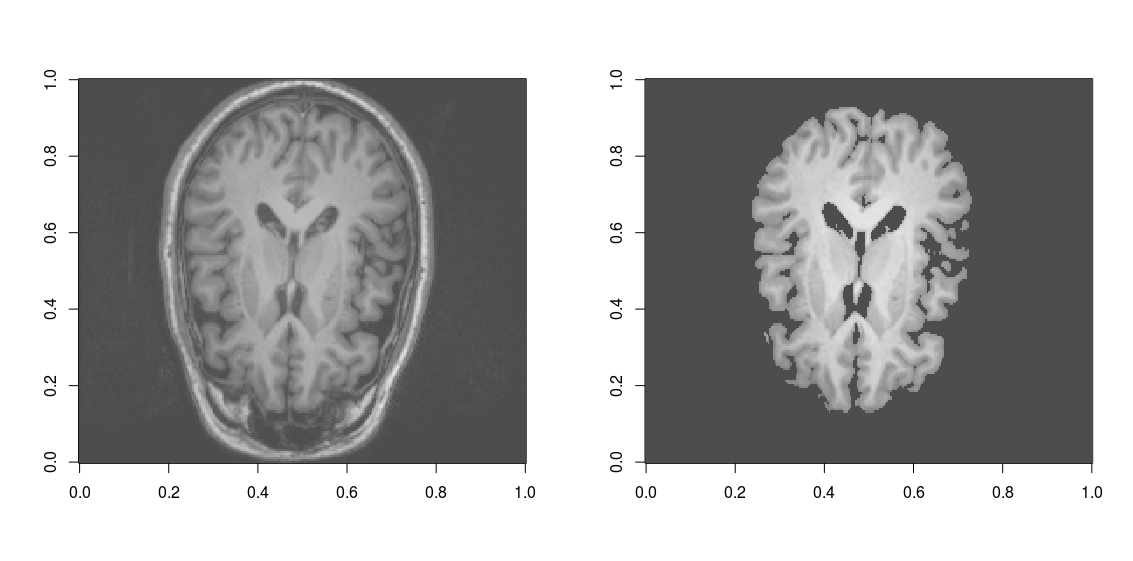
\includegraphics[width=\linewidth]{Images/6_t1_soft_eg.png}
\caption{Original T1-weighted image and the extracted soft tissue.}
\label{data-t1-soft-fig}
\end{figure}

The resulting images retain voxels that are likely to contain brain tissue. Other features, such as the skull and suspected \textsc{csf}, are given an intensity of zero. Lacunes are filled with fluid and so have a signal intensity similar to that of \textsc{csf}. Consequently, lacunes are removed by the soft tissue mask. The removed regions tend to have well-defined edges, which may aid in the identification of smaller lacunes. Note that lacunes are still visible in the \textsc{flair} images.

\section{Generating response arrays}\label{data-lacune}

The T1-weighted and \textsc{flair} scans were rated visually by trained clinicians in accordance to the \textsc{strive} criterion \cite{WardlawJ.M.2013Nsfr}. The clinicians visually analysed the scans slice by slice, identifying possible lacunes, perivascular spaces, and other lesions. Each lesion was analysed by a team of clinicians to confirm the identification. The rating of lacunes were then logged in Microsoft Excel, which also details the scan ID and the number of lacunes in each \textsc{mri} scan. For each lacune detected, the spreadsheet lists the axial slice ($y$-coordinate), diameter in millimetres, hemispheric location, and the ID of the surrounding brain structure. A sample of the spreadsheet data is shown in Table \ref{data-excel-tab}.

\begin{table}[ht]
	\centering
	\begin{tabular}{llllll}
	\toprule[1.5pt]
	Scan ID & No. of lacunes & Axial Slice & Diameter & Side & Region\\
	\midrule
	42 & 2 & 102 & 7 & L & 3 (Cortex)\\
	102 & 1 & 112 & 10 & R & 4 (Thalamus)\\
	\ldots\\
	\bottomrule[1.5pt]\\
	\end{tabular}
	\caption{Sample spreadsheet data. Each row describes one scan, identifying the size and location of lacunes. Each row contains repeated columns to describe multiple lacunes per scan ID.}
	\label{data-excel-tab}
\end{table}

The provided data describes the approximate anatomical location of lacunes. This format is not immediately usable to the model as it lacks precise coordinates. To resolve this, the spreadsheet was used as a guide to visually identify lacunes. Once found, an overlay of lacunes for the T1-weighted scans was generated such that each pixel in the image corresponds to a positive binary response.

\begin{figure}[ht]
\centering
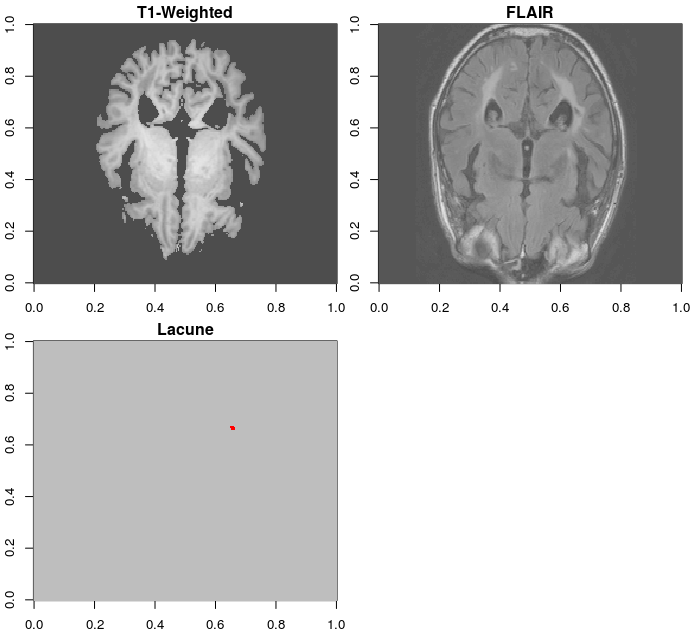
\includegraphics[width=\linewidth]{Images/6_lacune_mask.png}
\caption{Comparison of T1-weighted images, corresponding \textsc{flair} and lacune identification overlay (lacune in red).}
\label{data-t1-flair-lac}
\end{figure}

The responses were generated in FSLView, a program used by neuroscientists to view and annotate \textsc{mri} scans in the \texttt{.nifti} file format. For each brain scan described in the Excel spreadsheet, FSLView was used to generate a zero-initialised three-dimensional array of the same dimensions as the corresponding T1-weighted scan. Lacunes were visually identified by examining the indicated brain structure for lesions that appear dark in the T1-weighted images and with a hyperintense rim in the \textsc{flair} images. The empty arrays were opened in FSLView such that the voxels correspond to that of the T1-weighted images. The voxels that form the identified lacunes were indicated with ones using the Brush tool. These overlays were saved as \texttt{.nifti} files so they could be imported alongside the soft tissue and \textsc{flair} \texttt{.nifti} files. An example of a lacune overlay is shown in Figure \ref{data-t1-flair-lac}.



% Start descriptions of data - where it came from. Rating process and wave reviews. Data itself consisted of t1 and flair scans, and excel spreadhseet of slice numbers and sizes. To build the response values, an overlay was made for each scan. Overlays were built in fslview in the nifti format. Lacunes were identified using the guidance spreadsheet. A brush tool was used to fill 1s for lacunes. 0 elsewhere.

\section{Generating samples}\label{data-samples}

The candidate generation model by \cite{GhafoorianM.2017Dml3} specifies each sample to be 51$\times$51 axial images of both T1-weighting and \textsc{flair}. In their model, samples were chosen randomly such that positive lacune samples encompassed one-third of the data set. Data augmentation was used to increase the number of samples. In total, Ghafoorian et al. collected $3.2\times10^5$ training samples from 1,075 scans.

Our data set contains significantly fewer scans. In total the data set contains 411 \textsc{mri} scans, of which 35 contain lacunes. The scans were imported into R and converted into three-dimensional arrays using the AnalyzeFMRI package (v1.1-17). Each value of an array is the \textsc{mri} intensity at that voxel. Regions external to the scanned brain are given an intensity of zero.

The locations of the positive samples (lacunes) were extracted using the overlays generated in Section \ref{data-lacune}. For each nonzero value in the overlay, two 51$\times$51-dimensional arrays were created of T1-weighted and \textsc{flair} images. The pixel being classified occurs at the centre of each array. To increase sample size, additional augmented samples were formed by flipping the image horizontally. This method of sampling returned 3,846 lacune samples in total. Examples are shown in Figure \ref{data-positives}.

\begin{figure}[ht]
\centering
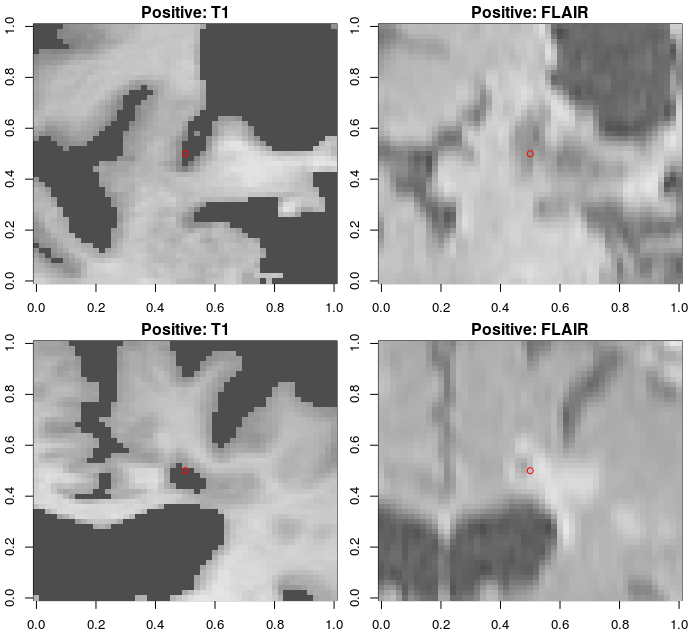
\includegraphics[width=\linewidth]{Images/6_positives.png}
\caption{Examples of positive samples. T1-weighted images and corresponding \textsc{flair}.}
\label{data-positives}
\end{figure}


\begin{figure}[ht]
\centering
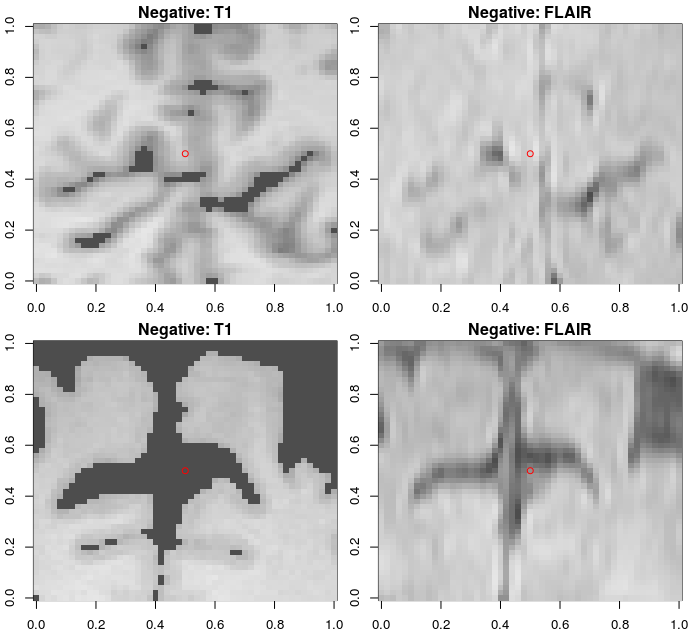
\includegraphics[width=\linewidth]{Images/6_negatives.png}
\caption{Examples of negative samples. T1-weighted images and corresponding \textsc{flair}.}
\label{data-negatives}
\end{figure}

Negative (non-lacune) samples were generated by considering voxels that return a negative response in the lacune overlay. The number of lacunes appearing in \textsc{mri} is fairly low, and each lacune has a diameter up to only 15 mm. Therefore, the number of potential negative samples vastly outnumbers positive samples. Given too many negative samples, the model will have a tendency to classify each given sample as negative without the cost function reporting large errors. For example, a data set containing 99\% negatives will return a 99\% classification accuracy for a model that outputs all points as negative.

Negative samples were chosen in intervals of 25 pixels with starting location chosen randomly. Samples were discarded if the central voxel was surrounded by a 4$\times$4$\times$4 empty volume, reducing the number of sparse samples. Examples are shown in Figure \ref{data-negatives}. This was used to generate a total of 39,983 negative samples. Positives samples make up 8.78\% of the dataset.

%\section{The Data}
%
%Where the data came from. The MRI source, type of images, with wavelengths etc. Similar description to Ghafoorian's (Section 2.1). Any preprocessing.
%
%What the samples were. E.g. 51x51 patches. Number of training, validation, testing.
%
%Show some example images, alongside their classification.
%
%The system that the models were built under - built in R using a tensorflow API. Models were run on dedicated servers.

%\section{First Model Structure}
%
%Code in Appendix.
%
%Purpose was to have a point of comparison against the model built by Ghafoorian et al. \cite{GhafoorianM.2017Dml3}.
%
%Brief outline of structure.
%
%Different number of samples. Far fewer lacunes in our dataset. Paper had 2/3 negatives, 1/3 positives. Our data consists of just under 10\% positives. Proposed model paper had 320K total samples. Our data has 50K, far fewer samples than the proposed model.
%
%In addition, around the 11th epoch, the training accuracy drops from near 100\% to near 0\%. This could be since the cross entropy has a log, and the algorithm attempts to take log(0). Introduce a small constant to achieve log(y + 1e-10).
%Getting NANs from the cross entropy function.
%
%
%\section{Proposed Model Structure}
%
%Code in Appendix.
%
%Explain structure of model, including diagram similar to that from Ghafoorian. Number of layers, number of neurons in each layer. What each layer was and the order. Method for chosen hyper-parameters. 


%%%%%%%%%%%%%%%%%%%%%%%%%%%%%%%%%%%%%%%%%%%%%%%%%%%%%%%%%%%%%%%%%%%%%%%%%%

%\clearpage

\addcontentsline{toc}{chapter}{References}

\bibliographystyle{apalike}
\bibliography{bibliography.bib}

%\bibliographystyle{apacite}
%\bibliography{mybib.bib}



%\documentclass[honours,12pt,twoside]{unswthesis}

\usepackage{afterpage}
\usepackage{amsfonts}
\usepackage{amsmath}
\usepackage{amssymb}
\usepackage{amsthm}
\usepackage[english]{babel}
\usepackage{graphicx}
\usepackage{natbib}
\usepackage[utf8]{inputenc}
\usepackage{latexsym}
\usepackage{url}
\usepackage{todonotes}
\usepackage{tikz}
\usepackage{pdfpages}
\usetikzlibrary{arrows}
\usepackage{float}

\usepackage{booktabs}
\renewcommand{\arraystretch}{1.2}


%%%%%%%%%%%%%%%%%%%%%%%%%%%%%%%%%%%%%%%%%%%%%%%%%%%%%%%%%%%%%%%%%
%
%  The following are some simple LaTeX macros to give some
%  commonly used letters in funny fonts. You may need more or less of
%  these
%
\newcommand{\R}{\mathbb{R}}
\newcommand{\Q}{\mathbb{Q}}
\newcommand{\C}{\mathbb{C}}
\newcommand{\N}{\mathbb{N}}
\newcommand{\F}{\mathbb{F}}
\newcommand{\PP}{\mathbb{P}}
\newcommand{\T}{\mathbb{T}}
\newcommand{\Z}{\mathbb{Z}}
\newcommand{\B}{\mathfrak{B}}
\newcommand{\BB}{\mathcal{B}}
\newcommand{\M}{\mathfrak{M}}
\newcommand{\X}{\mathfrak{X}}
\newcommand{\Y}{\mathfrak{Y}}
\newcommand{\CC}{\mathcal{C}}
\newcommand{\E}{\mathbb{E}}
\newcommand{\cP}{\mathcal{P}}
\newcommand{\cS}{\mathcal{S}}
\newcommand{\A}{\mathcal{A}}
\newcommand{\ZZ}{\mathcal{Z}}

%%%%%%%%%%%%%%%%%%%%%%%%%%%%%%%%%%%%%%%%%%%%%%%%%%%%%%%%%%%%%%%%%%%%%
%
% The following are much more esoteric commands that I have left in
% so that this file still processes. Use or delete as you see fit
%
\newcommand{\bv}[1]{\mbox{BV($#1$)}}
\newcommand{\comb}[2]{\left(\!\!\!\begin{array}{c}#1\\#2\end{array}\!\!\!\right)
}
\newcommand{\Lat}{{\rm Lat}}
\newcommand{\var}{\mathop{\rm var}}
\newcommand{\Pt}{{\mathcal P}}
\def\tr(#1){{\rm trace}(#1)}
\def\Exp(#1){{\mathbb E}(#1)}
\def\Exps(#1){{\mathbb E}\sparen(#1)}
\newcommand{\floor}[1]{\left\lfloor #1 \right\rfloor}
\newcommand{\ceil}[1]{\left\lceil #1 \right\rceil}
\newcommand{\hatt}[1]{\widehat #1}
\newcommand{\modeq}[3]{#1 \equiv #2 \,(\text{mod}\, #3)}
\newcommand{\rmod}{\,\mathrm{mod}\,}
\newcommand{\p}{\hphantom{+}}
\newcommand{\vect}[1]{\mbox{\boldmath $ #1 $}}
\newcommand{\reff}[2]{\ref{#1}.\ref{#2}}
\newcommand{\psum}[2]{\sum_{#1}^{#2}\!\!\!'\,\,}
\newcommand{\bin}[2]{\left( \begin{array}{@{}c@{}}
				#1 \\ #2
			\end{array}\right)	}
%
%  Macros - some of these are in plain TeX (gasp!)
%
\newcommand{\be}{($\beta$)}
\newcommand{\eqp}{\mathrel{{=}_p}}
\newcommand{\ltp}{\mathrel{{\prec}_p}}
\newcommand{\lep}{\mathrel{{\preceq}_p}}
\def\brack#1{\left \{ #1 \right \}}
\def\bul{$\bullet$\ }
\def\cl{{\rm cl}}
\let\del=\partial
\def\enditem{\par\smallskip\noindent}
\def\implies{\Rightarrow}
\def\inpr#1,#2{\t \hbox{\langle #1 , #2 \rangle} \t}
\def\ip<#1,#2>{\langle #1,#2 \rangle}
\def\lp{\ell^p}
\def\maxb#1{\max \brack{#1}}
\def\minb#1{\min \brack{#1}}
\def\mod#1{\left \vert #1 \right \vert}
\def\norm#1{\left \Vert #1 \right \Vert}
\def\paren(#1){\left( #1 \right)}
\def\qed{\hfill \hbox{$\Box$} \smallskip}
\def\sbrack#1{\Bigl \{ #1 \Bigr \} }
\def\ssbrack#1{ \{ #1 \} }
\def\smod#1{\Bigl \vert #1 \Bigr \vert}
\def\smmod#1{\bigl \vert #1 \bigr \vert}
\def\ssmod#1{\vert #1 \vert}
\def\sspmod#1{\vert\, #1 \, \vert}
\def\snorm#1{\Bigl \Vert #1 \Bigr \Vert}
\def\ssnorm#1{\Vert #1 \Vert}
\def\sparen(#1){\Bigl ( #1 \Bigr )}

\newcommand\blankpage{%
    \null
    \thispagestyle{empty}%
    \addtocounter{page}{-1}%
    \newpage}
    
%%%%%%%%%%%%%%%%%%%%%%%%%%%%%%%%%%%%%%%%%%%%%%%%%%%%%%%%%%%%%%
%
% These environments allow you to get nice numbered headings
%  for your Theorems, Definitions etc.  
%
%  Environments
%
%%%%%%%%%%%%%%%%%%%%%%%%%%%%%%%

\newtheorem{theorem}{Theorem}[section]
\newtheorem{lemma}[theorem]{Lemma}
\newtheorem{proposition}[theorem]{Proposition}
\newtheorem{corollary}[theorem]{Corollary}
\newtheorem{conjecture}[theorem]{Conjecture}
\newtheorem{definition}[theorem]{Definition}
\newtheorem{example}{Example}
\newtheorem{remark}[theorem]{Remark}
\newtheorem{question}[theorem]{Question}
\newtheorem{notation}[theorem]{Notation}
\numberwithin{equation}{section}

%\begin{document}

\chapter{Results}\label{results}

\section{Final model structure}

The final simplified model has a similar structure to that of Ghafoorian et al.'s candidate detection model \cite{GhafoorianM.2017Dml3}. The model structure is shown in Figure \ref{results-model-fig}. The input data contains two axial images: soft tissue extracted T1 and \textsc{flair} images. Each of the images has resolution 51$\times$51 pixels and is centred at the same coordinate. The model classifies the central pixel as either a positive or negative reading, formatted as a two-dimensional vector. A response of $(1,0)^\intercal$ indicates a positive (lacune) sample and $(0,1)^\intercal$ a negative (non-lacune) sample.

% Simplified model structure
\begin{figure}[ht]
	\centering
	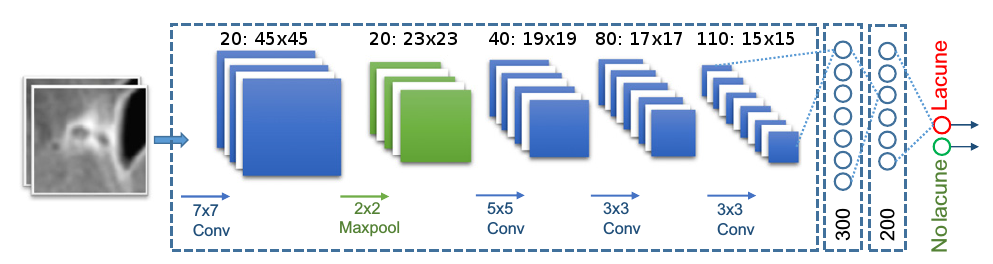
\includegraphics[width=\linewidth]{Images/7_simplified_model.png}
	\caption{Simplified model structure.}
	\small Image adapted from \cite{GhafoorianM.2017Dml3}
	\label{results-model-fig}
\end{figure}

The model consists of four convolutional layers of size 20, 40, 80 and 110, with filter sizes 7$\times$7, 5$\times$5, 3$\times$3 and 3$\times$3 respectively. A single max pooling layer is placed after the first convolutional layer, with size 2$\times$2 and stride 2. The convolutional layers are followed by three fully connected layers of size 300, 200 and 2. The final layer has softmax activation to output a probability distribution. All other layers have ReLU activation in order to avoid the vanishing gradient problem (see Section \ref{nnet-vanishinggradprob}). All neurons undergo batch normalisation and are initialised using the He method \cite{HeKaiming2015DDiR}. A dropout rate of 0.3 was applied to the fully connected layers.

Training was conducted using stochastic gradient descent with the Adam optimiser and a batch size of 128. A decaying learning rate was set from $5\times10^{-4}$ to $1\times10^{-6}$ by the 40th epoch. Cross-entropy loss was used with L2-regularisation, with the penalty rate set to $1\times10^{-4}$. An early stopping mechanism was implemented such that the model is tested against the validation set at the end of each epoch. If the validation accuracy improves, the model is saved. Once 40 epochs have run, the final saved model will have the highest validation accuracy.

Two models were trained using different positive-negative response ratios. The first model was developed using the positive-negative response ratio described by Ghafoorian et. al \cite{GhafoorianM.2017Dml3}: one third positive and two thirds negative. There are only 3846 positive samples in the MAS data set, allowing for a random selection of 7692 negative samples, thus giving a total sample size of 11538. These samples were split into three data sets: training, validation and testing. Splitting the data into these groups at a ratio of 50:25:25 yielded sample sizes 5769, 2884 and 2885 respectively.

The second model used the entire developed set of positive and negative lacune samples. This consisted of 3846 positive and 39983 negative samples to give a total sample size of 43829. Positive samples encompass 8.78\% of data samples. Similarly to the first data set, the data was split into training, validation and testing sets using a ratio of 50:25:25. This yielded sample sizes 21914, 10957 and 10958 respectively. All data sets were saved as R data files (\texttt{.Rda}).


\section{Training environment}

Model code was developed in R (v3.5.0) using RStudio (v1.1.453). The neural network was built and trained using Tensorflow (v1.10.0) through the R interface \texttt{tensorflow} (v1.8). The model was trained on a Linux machine running Ubuntu (release 16.04). The Tensorflow model was trained on the machine's CPU, an Intel(R) Core(TM) i7-4790 CPU 3.60GHz, with 16GB of RAM. 

\section{Results}

\subsection*{First model}

The first model generated has the same positive-negative sample ratio as outlined by Ghafoorian et. al \cite{GhafoorianM.2017Dml3}. The data consists of one-third positives and two-thirds negatives.

The model was trained for 40 epochs over 24 minutes, adjusting the network weights with each batch of 128 samples. Reusing the same data samples a large number of times introduces overfitting into the network \cite{Goodfellow-et-al-2016}. Overfitting can be observed when the accuracy of the training data set becomes very high, whereas the accuracy of the validation and testing data sets are low. Hence assessing model training accuracy can efficiently convey early model improvement; however it is not indicative of the model's performance when given new data.

Training accuracy was calculated every 5 batches, where each batch contained 128 samples. The resulting accuracies are shown in Figure \ref{results-train-acc4-fig}. There is a rapid increase in training accuracy within the first 100 batches. The model improvement occurs in steps as new features are found and more precise weight changes are made with the lowering learning rate \cite{Folly2009, Nielson2015}. The model reports a 100\% training accuracy consistently by batch 300. A majority of the model training occurs very early. In later training epochs, the training cost and learning rates are low and so the change in weights is also low (see Section \ref{nnets-backprop} on Backpropagation).

% Training accuracy
\begin{figure}[hb]
	\centering
	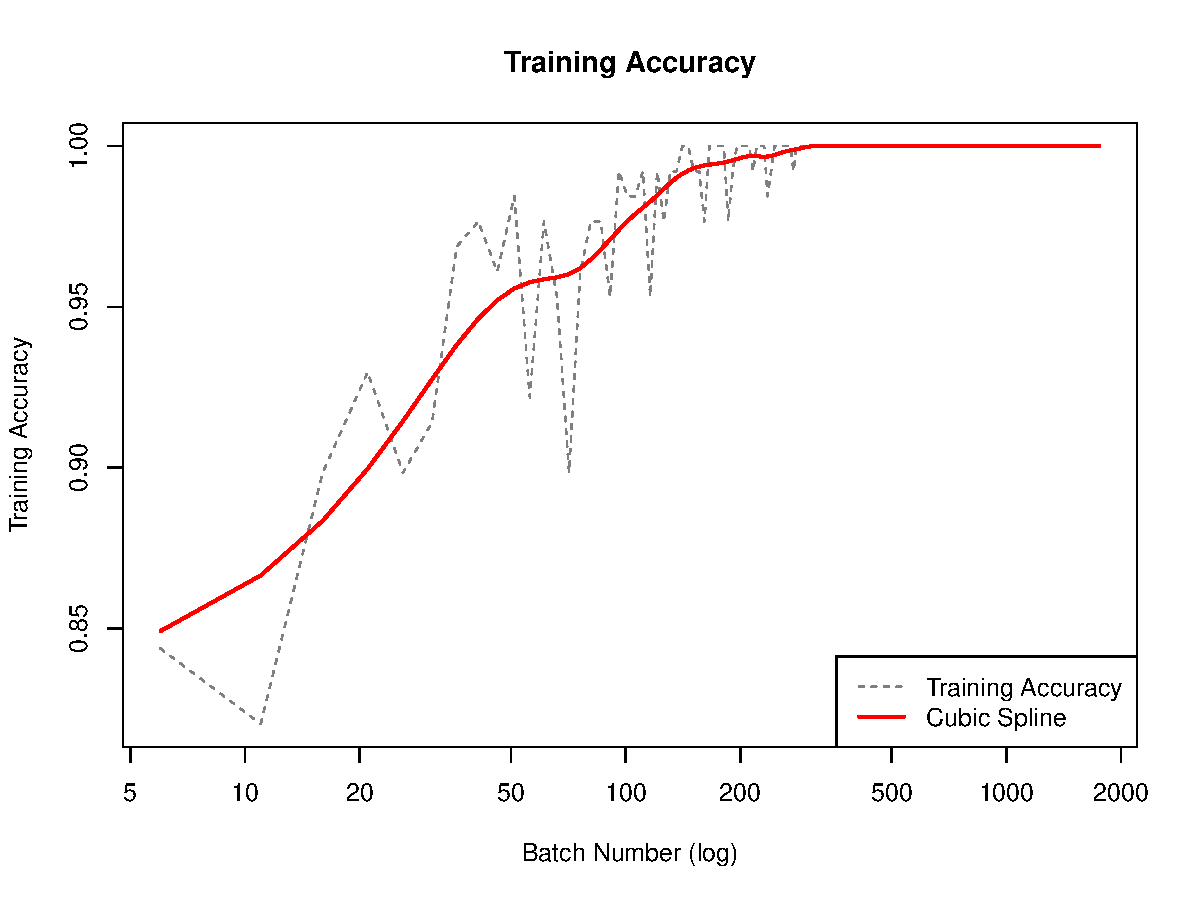
\includegraphics[width=\textwidth]{Images/7_train_acc4.pdf}
	\caption{Training data accuracy logged every 5 batches.}
	\label{results-train-acc4-fig}
\end{figure}

The model's validation set accuracy was tested after each epoch. This data set was not used for training and is used to assess the model's performance given new unseen data. The resulting validation accuracies are shown in Figure \ref{results-valid-acc4-fig}. Validation accuracy increases rapidly within the first 10 epochs. The maximum validation accuracy occurred at epochs 18, 22 and 25, achieving an accuracy of 0.992. The model was saved at epoch 18 to help minimise overfitting that may occur at later epochs. Applying this best validation accuracy model to the test data set resulted in an accuracy of 0.994.

% Validation accuracy
\begin{figure}[hb]
	\centering
	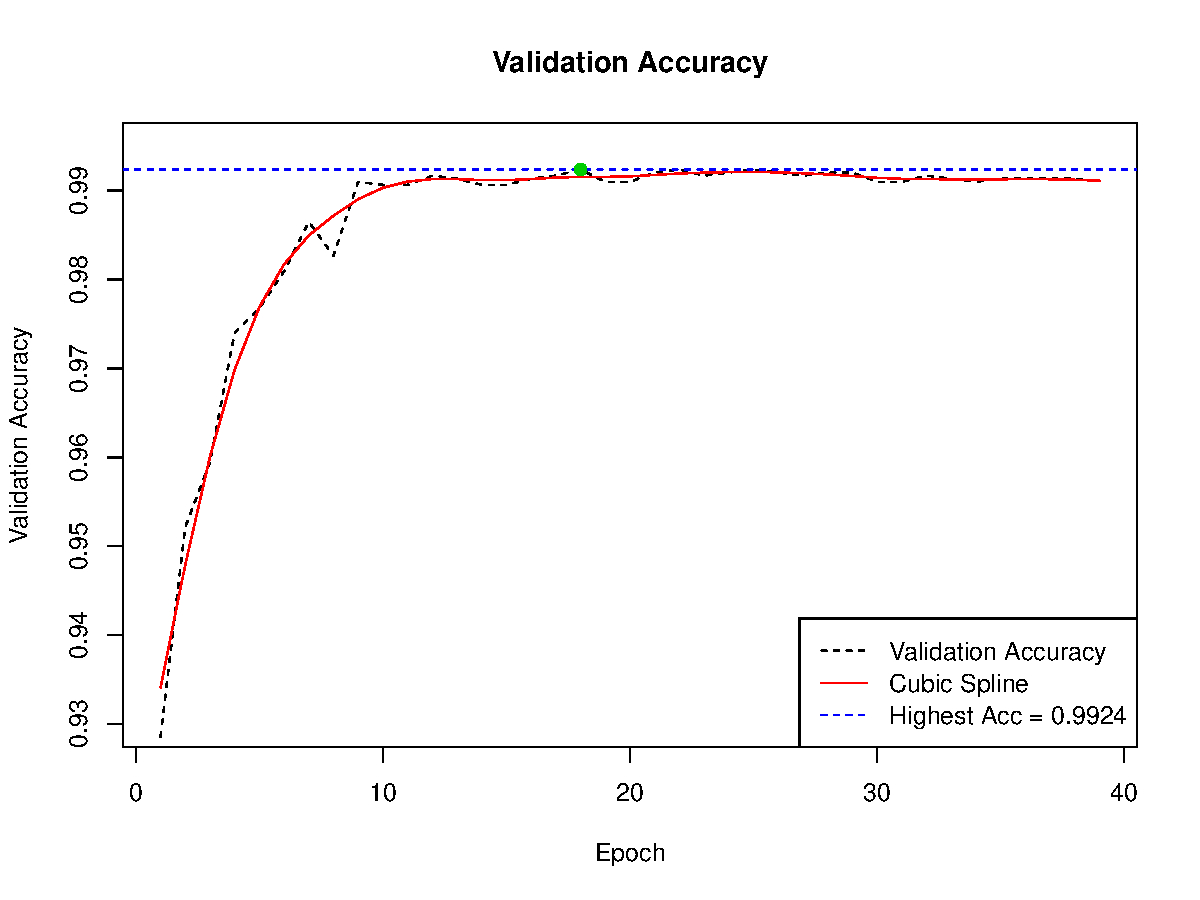
\includegraphics[width=\textwidth]{Images/7_valid_acc4.pdf}
	\caption{Validation data accuracy logged after each epoch.}
	\label{results-valid-acc4-fig}
\end{figure}

Though overall accuracy is a strong indicator of model performance, some types of inaccuracy can be more detrimental than others. In the identification of lacunes, it is preferable to have a larger number of false candidate lacunes than misclassify a true lacune. As a result, models will be compared by considering actual and predicted classification differences. Using this scheme, there are four outcomes: true-positive, true-negative, false-positive, and false-negative. These outcomes can be formatted into a \textit{confusion matrix}, as shown in Table \ref{results-confmat4-tab}.

\begin{table}[ht]
	\centering
	\begin{tabular}{@{}lll@{}}
	\toprule[1.5pt]
	& Positive & Negative\\
	\midrule
	True & 1004 & 1863\\
	False & 16 & 2\\
	\bottomrule[1.5pt]\\
	\end{tabular}
	\caption{Confusion matrix of the Model 1 testing data set.}
	\label{results-confmat4-tab}
\end{table}

The sensitivity of the model to lacunes is 99.6\% and specificity (correct classification of negative samples) of non-lacunes is 98.4\%.

\subsection*{Second model}

The second model was built using all of the generated positive and negative samples as described in Section \ref{data-samples}. The resulting training accuracy is shown in Figure \ref{results-train-acc5-fig}. The additional noise present in comparison to the previous model is the result of the larger sample size, rising from 5769 to 21914 samples. Note that the batch size and number of training epochs remained at 128 and 40 respectively, resulting in a larger number of batches processed during training. Model training duration was 85 minutes. The behaviour of this model was similar to that of the previous model, with a steep increase in training accuracy in early epochs followed by consistent correct classifications. Training accuracy was consistently at 100\% by batch 1000. 

% Training accuracy
\begin{figure}[ht]
	\centering
	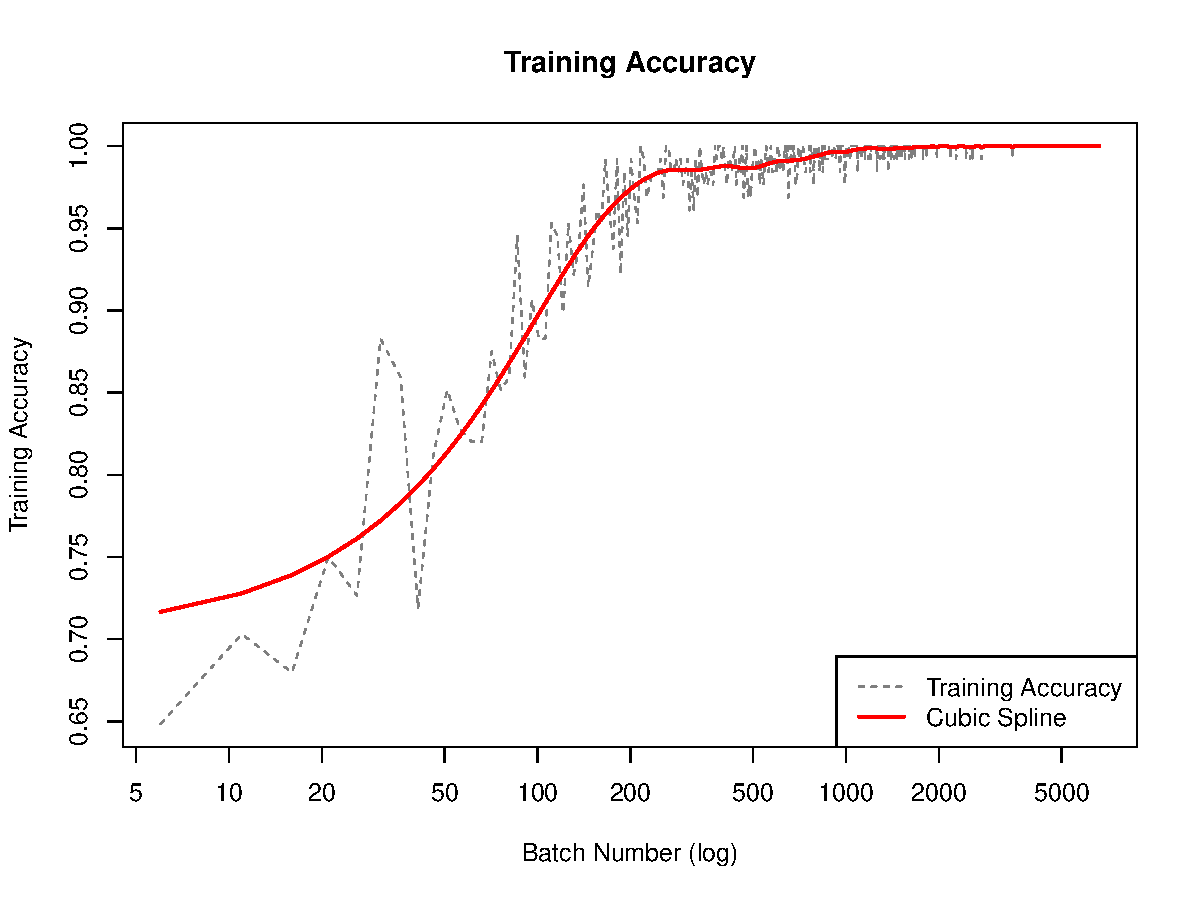
\includegraphics[width=\textwidth]{Images/7_train_acc5.pdf}
	\caption{Training data accuracy logged every 5 batches.}
	\label{results-train-acc5-fig}
\end{figure}

The performance of the model on the validation set is given in Figure \ref{results-valid-acc5-fig}. Validation accuracy was maximised at epochs 28 and 34, achieving an accuracy of 0.998. The model was saved at the earlier epoch 28 to reduce overfitting.

% Validation accuracy
\begin{figure}[ht]
	\centering
	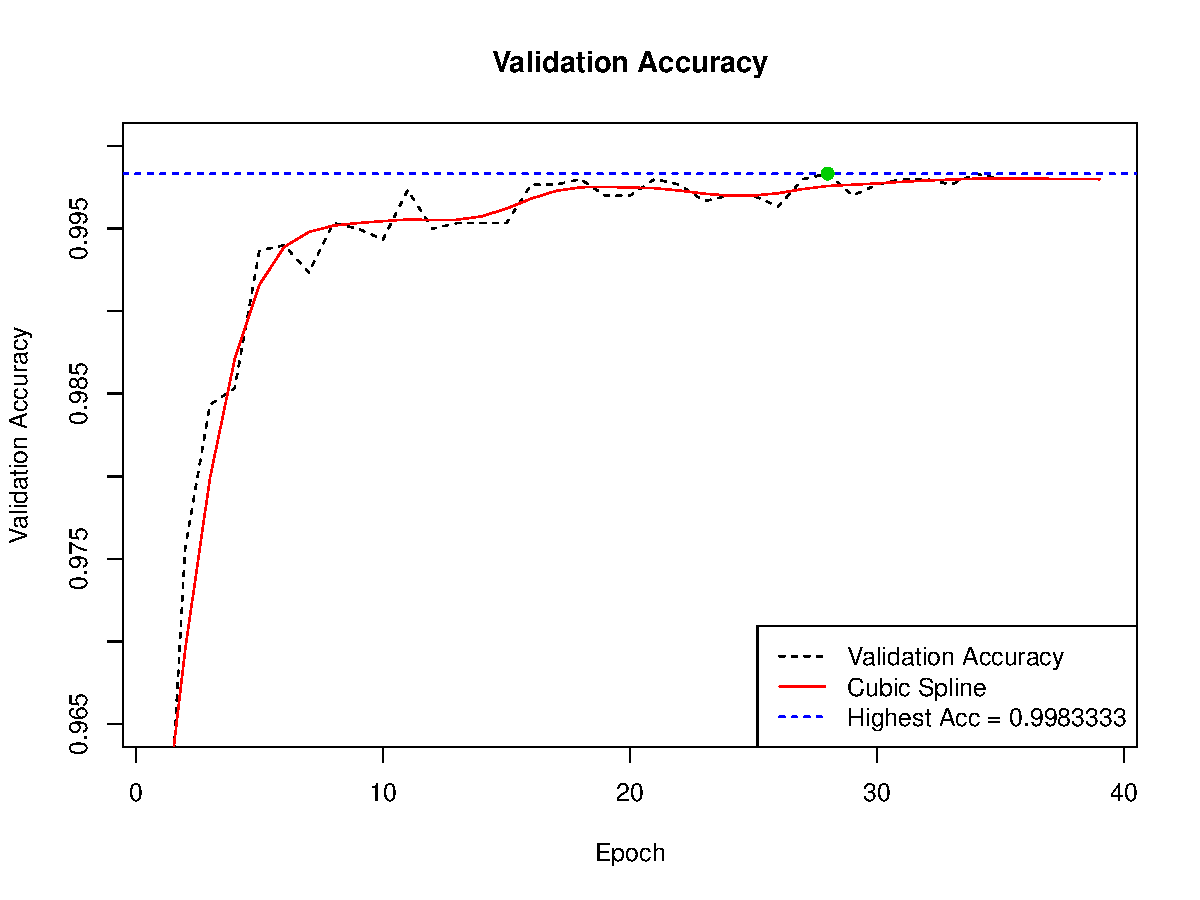
\includegraphics[width=\textwidth]{Images/7_valid_acc5.pdf}
	\caption{Validation data accuracy logged after each epoch}
	\label{results-valid-acc5-fig}
\end{figure}

Applying this best validation accuracy model to the test set achieved an accuracy of 99.8\%. The confusion matrix is given by Table \ref{results-confmat5-tab}, to give a sensitivity of 99.9\% and specificity of 99.7\%.

\begin{table}[ht]
	\centering
	\begin{tabular}{@{}lll@{}}
	\toprule[1.5pt]
	& Positive & Negative\\
	\midrule
	True & 961 & 9977\\
	False & 19 & 1\\
	\bottomrule[1.5pt]\\
	\end{tabular}
	\caption{Confusion matrix of the Model 2 testing data set.}
	\label{results-confmat5-tab}
\end{table}

\subsection*{Model comparisons}

The sensitivities and specificities of the two models are given in Table \ref{results-sens-spec-tab}. We observe that the second trained model has a higher sensitivity and specificity than that of the first model. We conduct a hypothesis test on the differences between the two models.

\begin{table}[ht]
	\centering
	\begin{tabular}{@{}lll@{}}
	\toprule[1.5pt]
	& Sensitivity & Specificity\\
	\midrule
	Model 1 & 0.9980 (1004/1006) & 0.9915 (1863/1879)\\
	Model 2 & 0.9990 (961/962) & 0.9981 (9977/9996)\\
	\bottomrule[1.5pt]\\
	\end{tabular}
	\caption{Sensitivities and specificities of both models.}
	\label{results-sens-spec-tab}
\end{table}

First, we test the difference in sensitivity proportions. The Central Limit Theorem (\textsc{clt}) is not applicable as the number of false-negatives is too small in both models. Instead, we use Fisher's Exact test. Let $X_1$ and $X_2$ be the number of lacunes correctly identified under the first and second models respectively. Let $n_1$ and $n_2$ be their respective sample sizes. Under the null hypothesis, for fixed $X_1 + X_2$, $X_1$ and $X_2$ have a hypergeometric distribution with probability
\begin{align*}
	P(X_1 = x_1, X_2 = x_2) = \dfrac{\dbinom{n_1}{x_1}\dbinom{n_2}{x_2}}{\dbinom{n_1 + n_2}{x_1 + x_2}}.
\end{align*}

The resulting p-value is 1, and we conclude that the two sensitivity proportions are not significantly different.

We now test the difference in specificity rates. We hypothesise that both sample proportions come from sampling distributions with the same probability. We can apply a $z$-test since we have sufficiently large number of observations and the data are independent. Let $X_1$ and $X_2$ be the number of correctly classified negative samples from the first and second models respectively. Let $n_1$ and $n_2$ be the total number of negative samples, so that $\hat{p}_1 = \dfrac{X_1}{n_1}$ and $\hat{p}_2 = \dfrac{X_2}{n_2}$ are the observed specificities. The observed pooled specificity proportion is
\begin{align*}
	\hat p_{pooled} = \dfrac{1863+9977}{1879+9996} = 0.9970526.
\end{align*}
From the \textsc{clt},
\begin{align*}
	Z = \dfrac{\hat{p}_1 - \hat{p}_2}{\sqrt{p_{pooled}(1 - p_{pooled})\left(\frac{1}{n_1} + \frac{1}{n_2}\right)}} \approx \mathcal{N}(0,1).
\end{align*}
The resulting test statistic is $z = -4.852599$. The probability of the observed proportion difference or lower is given by $P(Z < z) = 6.09\times10^{-7}$. This is well below the 5\% significance level and it is concluded that the specificity of the second model is higher than that of the first.

It has been proven that the model trained with the larger sample size and smaller proportion of positives did not affect sensitivity rates and increased specificity. 

\todo[inline]{Show examples of false-positives and true-negatives. What do these tend to look like?}

\todo[inline]{What happens when the scan is run on a whole brain?}

%\section{Reference Model Results}
%
%Results from running Ghafoorian's model. Training time, and final sensitivity and average false-positives per slice.
%
%\subsection*{Attempt1}
%
%training/testing in ratio 70:30. Here, only 7\% of data consists of positives. 41819 samples in total. Validation occurs on first 500 of the testing set. Training time: 02:04:48.
%Training accuracy achieved 100\% before batch 100x5. Validation accuracy peaked at epoch 8, with an accuracy of 100\%. Though should be noted that the size of this validation set consists of only 500 samples. Testing the whole testing set (15544 samples) achieves an accuracy of 0.9938.
%
%\subsection*{Attempt2}
%
%training/validation/testing in ratio 50:25:25. 1/3 of data was positives. 11539 samples in total. Training time: 00:23:11.
%Training accuracy achieved 100\% before batch 50x5. Validation accuracy peaked at epoch 21, which achieved an accuracy of 0.984055. Applying this best validation model to testing data achieved an accuracy of 0.9833622. Lower accuracy could be the result of fewer data points for training - caused by having only a limited number of positives in the original data set compared to the abundant negatives.
%
%\subsection*{Attempt3}
%
%Use original 7\% ratio. 41819 samples, with training/validation/testing in ratio 50:25:25. Have to be careful not to introduce too many negatives as this could impact what the model attempts to predict. E.g. if there are only 1\% positives, then an accuracy of 99\% could be achieved just by labelling all the samples as negative. Training time: 01:58:23.
%Training accuracy achieved 100\% before batch 100x5. Validation accuracy peaked at epoch 18, with an accuracy of 0.9979159, with the set containing 12955 samples. The testing set achieved an accuracy of 0.9972.
%
%\subsection*{Fixed Samples}
%
%Samples were changed. Previously, negative samples were chosen such that they were not lacunes, and also did not have a central pixel value of 0. However, some regions within the brain matter do have a central value of 0, and these can be some of the hardest points to distinguish.
%
%Negative sampling was changed to random points that were not lacunes, and the entire 9x9 central square is not 0 (to remove samples from outside the brain matter). 
%
%\subsection*{Attempt4}
%
%training/validation/testing in ratio 50:25:25. 1/3 of data was positives. 11538 samples in total. Training time: 00:22:51.
%Training accuracy achieved 100\% at batch 28x5. Consistent 100\% by batch 50x5. Validation accuracy peaked at epochs 31 and 34, achieving an accuracy of 0.9899445. Applying this best validation accuracy model to the test set achieved an accuracy of 0.9885615.
%
%Testing set was only 2885 samples. The number of true/false-positives and negatives were:
%TP: 972
%TN: 1879
%FP: 30
%FN: 4
%
%Sensitivity is 972/(972+4) = 99.6\% and specificity is 1879/(1879+30) = 98.4\%.
%
%
%
%\subsection*{Attempt5}
%
%training/validation/testing with 8.77\% positives. 43854 samples in total. Training time: 01:13:17. Training accuracy achieved 100\% at batch 41x5=205. Consistently 100\% at batch 150x5=750. Validation accuracy peaked at epoch 22, which achieved an accuracy of 0.9983581. Applying this best validation accuracy model to the test set achieved an accuracy of 0.9968989.
%Testing set comprised of 10964 samples. Of these, the number of true/false-positives and negatives were calculated:
%
%TP: 955
%TN: 9969
%FP: 33
%FN: 7
%
%Sensitivity is 955/(955+7) = 99.3\%, and specificity is 9969/(9969+33) = 99.7\%.

%%%%%%%%%%%%%%%%%%%%%%%%%%%%%%%%%%%%%%%%%%%%%%%%%%%%%%%%%%%%%%%%%%%%%%%%%%

%\clearpage

\addcontentsline{toc}{chapter}{References}

\bibliographystyle{apalike}
\bibliography{bibliography.bib}

%\bibliographystyle{apacite}
%\bibliography{mybib.bib}



\documentclass[honours,12pt,twoside]{unswthesis}

\usepackage{afterpage}
\usepackage{amsfonts}
\usepackage{amsmath}
\usepackage{amssymb}
\usepackage{amsthm}
\usepackage[english]{babel}
\usepackage{graphicx}
\usepackage{natbib}
\usepackage[utf8]{inputenc}
\usepackage{latexsym}
\usepackage{url}
\usepackage{todonotes}
\usepackage{tikz}
\usepackage{pdfpages}
\usetikzlibrary{arrows}
\usepackage{float}

\usepackage{booktabs}
\renewcommand{\arraystretch}{1.2}


%%%%%%%%%%%%%%%%%%%%%%%%%%%%%%%%%%%%%%%%%%%%%%%%%%%%%%%%%%%%%%%%%
%
%  The following are some simple LaTeX macros to give some
%  commonly used letters in funny fonts. You may need more or less of
%  these
%
\newcommand{\R}{\mathbb{R}}
\newcommand{\Q}{\mathbb{Q}}
\newcommand{\C}{\mathbb{C}}
\newcommand{\N}{\mathbb{N}}
\newcommand{\F}{\mathbb{F}}
\newcommand{\PP}{\mathbb{P}}
\newcommand{\T}{\mathbb{T}}
\newcommand{\Z}{\mathbb{Z}}
\newcommand{\B}{\mathfrak{B}}
\newcommand{\BB}{\mathcal{B}}
\newcommand{\M}{\mathfrak{M}}
\newcommand{\X}{\mathfrak{X}}
\newcommand{\Y}{\mathfrak{Y}}
\newcommand{\CC}{\mathcal{C}}
\newcommand{\E}{\mathbb{E}}
\newcommand{\cP}{\mathcal{P}}
\newcommand{\cS}{\mathcal{S}}
\newcommand{\A}{\mathcal{A}}
\newcommand{\ZZ}{\mathcal{Z}}

%%%%%%%%%%%%%%%%%%%%%%%%%%%%%%%%%%%%%%%%%%%%%%%%%%%%%%%%%%%%%%%%%%%%%
%
% The following are much more esoteric commands that I have left in
% so that this file still processes. Use or delete as you see fit
%
\newcommand{\bv}[1]{\mbox{BV($#1$)}}
\newcommand{\comb}[2]{\left(\!\!\!\begin{array}{c}#1\\#2\end{array}\!\!\!\right)
}
\newcommand{\Lat}{{\rm Lat}}
\newcommand{\var}{\mathop{\rm var}}
\newcommand{\Pt}{{\mathcal P}}
\def\tr(#1){{\rm trace}(#1)}
\def\Exp(#1){{\mathbb E}(#1)}
\def\Exps(#1){{\mathbb E}\sparen(#1)}
\newcommand{\floor}[1]{\left\lfloor #1 \right\rfloor}
\newcommand{\ceil}[1]{\left\lceil #1 \right\rceil}
\newcommand{\hatt}[1]{\widehat #1}
\newcommand{\modeq}[3]{#1 \equiv #2 \,(\text{mod}\, #3)}
\newcommand{\rmod}{\,\mathrm{mod}\,}
\newcommand{\p}{\hphantom{+}}
\newcommand{\vect}[1]{\mbox{\boldmath $ #1 $}}
\newcommand{\reff}[2]{\ref{#1}.\ref{#2}}
\newcommand{\psum}[2]{\sum_{#1}^{#2}\!\!\!'\,\,}
\newcommand{\bin}[2]{\left( \begin{array}{@{}c@{}}
				#1 \\ #2
			\end{array}\right)	}
%
%  Macros - some of these are in plain TeX (gasp!)
%
\newcommand{\be}{($\beta$)}
\newcommand{\eqp}{\mathrel{{=}_p}}
\newcommand{\ltp}{\mathrel{{\prec}_p}}
\newcommand{\lep}{\mathrel{{\preceq}_p}}
\def\brack#1{\left \{ #1 \right \}}
\def\bul{$\bullet$\ }
\def\cl{{\rm cl}}
\let\del=\partial
\def\enditem{\par\smallskip\noindent}
\def\implies{\Rightarrow}
\def\inpr#1,#2{\t \hbox{\langle #1 , #2 \rangle} \t}
\def\ip<#1,#2>{\langle #1,#2 \rangle}
\def\lp{\ell^p}
\def\maxb#1{\max \brack{#1}}
\def\minb#1{\min \brack{#1}}
\def\mod#1{\left \vert #1 \right \vert}
\def\norm#1{\left \Vert #1 \right \Vert}
\def\paren(#1){\left( #1 \right)}
\def\qed{\hfill \hbox{$\Box$} \smallskip}
\def\sbrack#1{\Bigl \{ #1 \Bigr \} }
\def\ssbrack#1{ \{ #1 \} }
\def\smod#1{\Bigl \vert #1 \Bigr \vert}
\def\smmod#1{\bigl \vert #1 \bigr \vert}
\def\ssmod#1{\vert #1 \vert}
\def\sspmod#1{\vert\, #1 \, \vert}
\def\snorm#1{\Bigl \Vert #1 \Bigr \Vert}
\def\ssnorm#1{\Vert #1 \Vert}
\def\sparen(#1){\Bigl ( #1 \Bigr )}

\newcommand\blankpage{%
    \null
    \thispagestyle{empty}%
    \addtocounter{page}{-1}%
    \newpage}
    
%%%%%%%%%%%%%%%%%%%%%%%%%%%%%%%%%%%%%%%%%%%%%%%%%%%%%%%%%%%%%%
%
% These environments allow you to get nice numbered headings
%  for your Theorems, Definitions etc.  
%
%  Environments
%
%%%%%%%%%%%%%%%%%%%%%%%%%%%%%%%

\newtheorem{theorem}{Theorem}[section]
\newtheorem{lemma}[theorem]{Lemma}
\newtheorem{proposition}[theorem]{Proposition}
\newtheorem{corollary}[theorem]{Corollary}
\newtheorem{conjecture}[theorem]{Conjecture}
\newtheorem{definition}[theorem]{Definition}
\newtheorem{example}{Example}
\newtheorem{remark}[theorem]{Remark}
\newtheorem{question}[theorem]{Question}
\newtheorem{notation}[theorem]{Notation}
\numberwithin{equation}{section}

\begin{document}

\chapter{Conclusion}\label{conclusion}

R

\citep{AdamsH.H.Hieab2013RMfD}



%%%%%%%%%%%%%%%%%%%%%%%%%%%%%%%%%%%%%%%%%%%%%%%%%%%%%%%%%%%%%%%%%%%%%%%%%%

\clearpage

\addcontentsline{toc}{chapter}{References}

\bibliographystyle{apalike}
\bibliography{bibliography.bib}

%\bibliographystyle{apacite}
%\bibliography{mybib.bib}



%\documentclass[honours,12pt,twoside]{unswthesis}

\usepackage{afterpage}
\usepackage{amsfonts}
\usepackage{amsmath}
\usepackage{amssymb}
\usepackage{amsthm}
\usepackage[english]{babel}
\usepackage{graphicx}
\usepackage{natbib}
\usepackage[utf8]{inputenc}
\usepackage{latexsym}
\usepackage{url}
\usepackage{todonotes}
\usepackage{tikz}
\usepackage{pdfpages}
\usetikzlibrary{arrows}
\usepackage{float}

\usepackage{booktabs}
\renewcommand{\arraystretch}{1.2}


%%%%%%%%%%%%%%%%%%%%%%%%%%%%%%%%%%%%%%%%%%%%%%%%%%%%%%%%%%%%%%%%%
%
%  The following are some simple LaTeX macros to give some
%  commonly used letters in funny fonts. You may need more or less of
%  these
%
\newcommand{\R}{\mathbb{R}}
\newcommand{\Q}{\mathbb{Q}}
\newcommand{\C}{\mathbb{C}}
\newcommand{\N}{\mathbb{N}}
\newcommand{\F}{\mathbb{F}}
\newcommand{\PP}{\mathbb{P}}
\newcommand{\T}{\mathbb{T}}
\newcommand{\Z}{\mathbb{Z}}
\newcommand{\B}{\mathfrak{B}}
\newcommand{\BB}{\mathcal{B}}
\newcommand{\M}{\mathfrak{M}}
\newcommand{\X}{\mathfrak{X}}
\newcommand{\Y}{\mathfrak{Y}}
\newcommand{\CC}{\mathcal{C}}
\newcommand{\E}{\mathbb{E}}
\newcommand{\cP}{\mathcal{P}}
\newcommand{\cS}{\mathcal{S}}
\newcommand{\A}{\mathcal{A}}
\newcommand{\ZZ}{\mathcal{Z}}

%%%%%%%%%%%%%%%%%%%%%%%%%%%%%%%%%%%%%%%%%%%%%%%%%%%%%%%%%%%%%%%%%%%%%
%
% The following are much more esoteric commands that I have left in
% so that this file still processes. Use or delete as you see fit
%
\newcommand{\bv}[1]{\mbox{BV($#1$)}}
\newcommand{\comb}[2]{\left(\!\!\!\begin{array}{c}#1\\#2\end{array}\!\!\!\right)
}
\newcommand{\Lat}{{\rm Lat}}
\newcommand{\var}{\mathop{\rm var}}
\newcommand{\Pt}{{\mathcal P}}
\def\tr(#1){{\rm trace}(#1)}
\def\Exp(#1){{\mathbb E}(#1)}
\def\Exps(#1){{\mathbb E}\sparen(#1)}
\newcommand{\floor}[1]{\left\lfloor #1 \right\rfloor}
\newcommand{\ceil}[1]{\left\lceil #1 \right\rceil}
\newcommand{\hatt}[1]{\widehat #1}
\newcommand{\modeq}[3]{#1 \equiv #2 \,(\text{mod}\, #3)}
\newcommand{\rmod}{\,\mathrm{mod}\,}
\newcommand{\p}{\hphantom{+}}
\newcommand{\vect}[1]{\mbox{\boldmath $ #1 $}}
\newcommand{\reff}[2]{\ref{#1}.\ref{#2}}
\newcommand{\psum}[2]{\sum_{#1}^{#2}\!\!\!'\,\,}
\newcommand{\bin}[2]{\left( \begin{array}{@{}c@{}}
				#1 \\ #2
			\end{array}\right)	}
%
%  Macros - some of these are in plain TeX (gasp!)
%
\newcommand{\be}{($\beta$)}
\newcommand{\eqp}{\mathrel{{=}_p}}
\newcommand{\ltp}{\mathrel{{\prec}_p}}
\newcommand{\lep}{\mathrel{{\preceq}_p}}
\def\brack#1{\left \{ #1 \right \}}
\def\bul{$\bullet$\ }
\def\cl{{\rm cl}}
\let\del=\partial
\def\enditem{\par\smallskip\noindent}
\def\implies{\Rightarrow}
\def\inpr#1,#2{\t \hbox{\langle #1 , #2 \rangle} \t}
\def\ip<#1,#2>{\langle #1,#2 \rangle}
\def\lp{\ell^p}
\def\maxb#1{\max \brack{#1}}
\def\minb#1{\min \brack{#1}}
\def\mod#1{\left \vert #1 \right \vert}
\def\norm#1{\left \Vert #1 \right \Vert}
\def\paren(#1){\left( #1 \right)}
\def\qed{\hfill \hbox{$\Box$} \smallskip}
\def\sbrack#1{\Bigl \{ #1 \Bigr \} }
\def\ssbrack#1{ \{ #1 \} }
\def\smod#1{\Bigl \vert #1 \Bigr \vert}
\def\smmod#1{\bigl \vert #1 \bigr \vert}
\def\ssmod#1{\vert #1 \vert}
\def\sspmod#1{\vert\, #1 \, \vert}
\def\snorm#1{\Bigl \Vert #1 \Bigr \Vert}
\def\ssnorm#1{\Vert #1 \Vert}
\def\sparen(#1){\Bigl ( #1 \Bigr )}

\newcommand\blankpage{%
    \null
    \thispagestyle{empty}%
    \addtocounter{page}{-1}%
    \newpage}
    
%%%%%%%%%%%%%%%%%%%%%%%%%%%%%%%%%%%%%%%%%%%%%%%%%%%%%%%%%%%%%%
%
% These environments allow you to get nice numbered headings
%  for your Theorems, Definitions etc.  
%
%  Environments
%
%%%%%%%%%%%%%%%%%%%%%%%%%%%%%%%

\newtheorem{theorem}{Theorem}[section]
\newtheorem{lemma}[theorem]{Lemma}
\newtheorem{proposition}[theorem]{Proposition}
\newtheorem{corollary}[theorem]{Corollary}
\newtheorem{conjecture}[theorem]{Conjecture}
\newtheorem{definition}[theorem]{Definition}
\newtheorem{example}{Example}
\newtheorem{remark}[theorem]{Remark}
\newtheorem{question}[theorem]{Question}
\newtheorem{notation}[theorem]{Notation}
\numberwithin{equation}{section}

%\begin{document}

\chapter{Appendix}\label{appendex}

Place code here

\citep{AdamsH.H.Hieab2013RMfD}



%%%%%%%%%%%%%%%%%%%%%%%%%%%%%%%%%%%%%%%%%%%%%%%%%%%%%%%%%%%%%%%%%%%%%%%%%%

%\clearpage

\addcontentsline{toc}{chapter}{References}

\bibliographystyle{apalike}
\bibliography{bibliography.bib}

%\bibliographystyle{apacite}
%\bibliography{mybib.bib}




%%%%%%%%%%%%%%%%%%%%%%%%%%%%%%%%%%%%%%%%%%%%%%%%%%%%%%%%%%%%%%%%%%%%%%%%%%

\clearpage

\addcontentsline{toc}{chapter}{References}

\bibliographystyle{apalike}
\bibliography{bibliography.bib}

%\bibliographystyle{apacite}
%\bibliography{mybib.bib}






